\documentclass[12pt,a4paper]{report}

\usepackage{dolgozat}

\usepackage{hyperref}

\usepackage{listings}
\usepackage{python}
\usepackage{cpp}

\usepackage{wrapfig}

\linespread{1.2}

\begin{document}

\pagestyle{empty} %a címlapon ne legyen semmi=empty, azaz nincs fejléc és lábléc

\begin{flushleft}
\textsc{\bfseries Miskolci Egyetem}\\
Gépészmérnöki és Informatikai Kar\\
Általános Informatikai Intézeti Tanszék
\end{flushleft}

%A fõiskola logoja
{\large
\begin{center}
\vglue 1truecm
\textbf{\huge\textsc{Szakdolgozat}}\\
\vglue 1truecm

\epsfig{file=cimlap/ME_logo.eps, width=4.8truecm, height=4truecm}\\
\textbf{\textsc{Miskolci Egyetem}}
\end{center}}

\vglue 1.5truecm %függõleges helykihagyás

%A szakdolgozat címe, akár több sorban is
{\LARGE
\begin{center}
\textbf{Tűzzel kapcsolatos jelenségek grafikus megjelenítése}
\end{center}}

\vspace*{2.5truecm}
%A hallgató neve, évfolyam, szak(ok), a konzulens(ek) neve
{\large
\begin{center}
\begin{tabular}{c}
\textbf{Készítette:}\\
Fodor Tamás János\\
Mérnökinformatikus BSc
\end{tabular}
\end{center}
\begin{center}
\begin{tabular}{c}
\textbf{Témavezető:}\\
Piller Imre, egyetemi tanársegéd
\end{tabular}
\end{center}}
\vfill
%Keltezés: Hely és év
{\large
\begin{center}
\textbf{\textsc{Miskolc, 2018}}
\end{center}}

\newpage


\cleardoublepage
\pagenumbering{gobble}
\tableofcontents
\cleardoublepage
\pagenumbering{arabic}

\newpage

\pagestyle{fancy}

\Chapter{Bevezetés}

A tűz úgy írható le, mint egy éghető anyag gyors, önfenntartó oxidációs folyamata. Ez az egyik legfontosabb és az egyik legszebb természeti jelenség, melynek számítógépi grafikai megjelenítése a mai napig nagy kihívást jelent, ha valós idejű, valósághű szimulációt szeretnénk elérni. Számítógépi megjelenítését széles körben alkalmazzák, többek között a mozifilmek speciális effektjeiben, tudományos szimulációkban, videojátékokban, stb. \cite{steinemannFire}.

A tűz különféle megjelenítési módjait a grafikában két egyszerűbb részre lehet osztani. Az első kategóriába tartoznak azok a 2 dimenziós renderelési technikák, melyek textúrák sorozatát használják a megjelenítéshez. Ezek a sorozatok lehetnek valós, generált vagy egyéb módon megalkotott képek, s gyakran egy \textit{billboardon} (sík lap, amely a rá húzott textúrának biztosít felületet) jelenítik meg őket. A legkifinomultabb verziók felhasználnak még Perlin zajt, vagy más, hasonló megközelítést a tűz dinamikájának érzékeltetéséhez. Leginkább torkolattűz vagy rövidebb robbanás megjelenítésére alkalmas, néhány fényforrást elhelyezve körülötte pedig tovább növelhető a valószerűsége, alacsonyan tartva a számítási igényt. Ezen módszerek előnye, hogy könnyű őket 3 dimenziós környezetben implementálni, így széles körben felhasználhatók, de gyakran nem tűnnek valóságosnak a 3D-s környezetben. Másrészt, a textúrákat mindig vagy merőlegesen kell kirajzolni a nézőpont irányára, vagy pedig a már renderelt képre kell leképezni őket. További hiányossága ezen módszereknek, hogy nem adnak lehetőséget a tűzzel való interakcióra, mint ahogy az egy virtuális valóságban elvárható lenne \cite{steinemannFire}.

A második kategóriába a 3D-s technológiák tartoznak. Ezek legfőbb előnye, hogy valósághűbb eredményeket produkálnak a következő pontokban
\begin{itemize}
\item vizuális megjelenés és dinamika,
\item a hőterjedés és hőtágulás modellezése,
\item más objektumokkal való interakció
\end{itemize}
tekintetében. A legnagyobb problémát ebben a kategóriában az égő gázok reprezentálása és modellezése a lángokban, a termodinamikájuk modellje és a renderelési módszer kiválasztása okozza.
Rengeteg különféle módszert dolgoztak már ki a tűz megjelenítésére, többek között: részecske-, folyadék- és láng-alapú modelleket. \cite{steinemannFire}. A dolgozat célja ezen módszerek bemutatása.

\Chapter{A tűz megjelenítése}

% TODO: Összeszedni az eddigi eredményeket a tűz megjelenítésével kapcsolatban!

\section{Megvalósítás a fontosabb játék motorokban}

A háromdimenziós játékok felemelkedése az 1990-es években kezdődött. Az első játékmotorok az id Software feljelszőinek köszönhetőek. Ahelyett, hogy minden játékot egyenként a semmiből építettek volna fel, más fejlesztők által készített modulokat használtak fel. Megtervezték a saját grafikájukat, karaktereiket, fegyvereiket és pályáikat, melyek lényegében a játék tartalmát nyújtották. Így már szét lehetett választani a játékspecifikus szabályokat és adatokat olyan alap koncepcióktól, mint például az ütközésvizsgálat. Ennek köszönhetően a fejlesztői csapatokat lehetett bővíteni, hiszen egyszerre több modulon is lehetett párhuzamosan, egymástól függetlenül dolgozni. Ez lehetővé tette továbbá, hogy a fejlesztők külön területekre specializálódjanak.
\cite{wikiGameEngine}

%Sprite tűz:
%1992 wolfeinsein 3d (id software)
%1993 id tech 1/doom engine https://en.wikipedia.org/wiki/Doom_engine +  https://doomwiki.org/wiki/Doom_rendering_engine 
% Doom II: Hell on Earth (id tech 1 ez is)

\subsection{Quake engine 1996}

% 1996 Quake engine 
% 1997 Quake II engine = id tech 2
% 1998 Unreal engine 1
% 1999 id tech 3 engine 
% 2002 Unreal engine 2
% 2004 id tech 4 engine 
% 2004 CryEngine 1 https://github.com/AFCStudio/CRYENGINE-1
% 2007 Unreal engine 3
% 2012 Unreal engine 4 
% 2017 CRYENGINE 5.4.0 https://github.com/CRYTEK/CRYENGINE


% Not open source:
% 2012 Gamebryo 4.0  https://en.wikipedia.org/wiki/Gamebryo
% RenderWare https://en.wikipedia.org/wiki/RenderWare
% Fork_Particle https://en.wikipedia.org/wiki/Fork_Particle
% Source https://en.wikipedia.org/wiki/Source_(game_engine)
% Creation Engine https://en.wikipedia.org/wiki/Creation_Engine
% Crystal Tools https://en.wikipedia.org/wiki/Crystal_Tools
% Enigma Engine https://en.wikipedia.org/wiki/Enigma_Engine
% Frostbite https://en.wikipedia.org/wiki/Frostbite_(game_engine)
% GoldSrc https://en.wikipedia.org/wiki/GoldSrc
% IW engine https://en.wikipedia.org/wiki/IW_engine
% Jade https://en.wikipedia.org/wiki/Jade_(game_engine)
% RenderWare https://en.wikipedia.org/wiki/RenderWare
% Riot engine https://en.wikipedia.org/wiki/Riot_Engine
% RAGE https://en.wikipedia.org/wiki/Rockstar_Advanced_Game_Engine
% Vision https://en.wikipedia.org/wiki/Vision_(game_engine)#Games_using_Vision_Engine
% 2011 id tech 5 
% 2016 id tech 666


\Chapter{A tűz fizikája}

% TODO: Leírni, hogy a tűz fizikája (beleértve a megjelenítés optikáját) hogyan működik nagyvonalakban!

\section{A tűz természetéből fakadó nehézségek}
Az égést, mint kémiai jelenséget, még ha ismernénk is minden részletet sem tudnánk elfogadható időn belül szimulálni  \cite{firestarter}.

A tűz a jelenetek egyik drámai eleme, így azt a lehető legnagyobb szinten kell tudni befolyásolni amellett, hogy közben hiteles is maradjon. Kiszámíthatatlannak és összetettnek kell tűnnie, ugyanakkor az adott körülményeknek megfelelően felismerhető struktúrájúnak kell lennie. Ebből a bonyolultságból és a szemlélői elvárásokból kifolyólag nem túl életképes a tűz animálása közvetlen numerikus szimuláció segítségével, ugyanis:
\begin{itemize}
\item
A numerikus szimulációk nagyban függenek a részletesség szintjétől. Ahogy egy 3D-s szimuláció felbontása finomodik, a számítási összetettsége legalább $O(n^3)$ szerint nő. Ha akár csak egy kisebb tüzet is szeretnénk részleteiben megjeleníteni, az nagyon magas számítási igényű rendereléshez vezet.
\item
Azok a (nagy számú) faktorok, melyek a tűz megjelenését határozzák meg különféle körülmények között, egy egymástól függő paraméterekből álló teret alkotnak. Ilyen fizikai rendszerre nehéz olyan függvényeket írni, melyek segítségével könnyen lehetne befolyásolni a tüzet. 
\item
A tűz maga a zűrzavar. Apró változtatások a kiinduló környezetben rendkívül eltérő eredményeket produkálnak. Az animálás szemszögéből nehéz egy kívánt eredmény felé terelni a folyamatokat \cite{ArNiStructuralModeling}.
\end{itemize}

Más-más alkalmazási területek különféle szempontokat tartanak szem előtt, mikor a tűz természetéről, megjelenéséről, és a megjelenítési időről van szó. Például:

Egy videojátékban az elsődleges szempont hogy valós időben (25-60 frame per secundum) lehessen renderelni a jelenséget, a kinézetnek is a lehetőségek szerint valóságosnak kell tűnnie. A legtöbb esetben csupán díszítő funkciót tölt be, így a terjedés fizikája és az interakció kevésbé lényeges.

Egy mozifilmben a legfontosabb, hogy minél élethűbb legyen, és esetlegesen lehessen kontrollálni a kinézetét. A renderelésnek itt már nem kell valós idejűnek lennie, illetve sem a tűz terjedésének fizikája, sem a vele való interakció nem játszik szerepet.

Egy virtuális valóságban - például egy tűzoltó szimulációs szoftverben - ismét szempont a valós idejű renderelés, de itt a tűzzel való interakció lehetősége és a terjedésének fizikája egyaránt fontosabb, mint maga a megjelenés.

\Chapter{Tűz modellek}

% TODO: Leírni, hogy milyen saját tűzmodellek implementálására fog majd sor kerülni!
% TODO: Alcímek legyenek?

\section{Kétdimenziós tűz textúrák segítségével}

A legegyszerűbb, legrégebb óta használt megjelenítési módszer 2D-s textúrák felhasználásával készül. Ebben fizikai modellek nem igazán kapnak helyet, inkább a látványvilág tervezőinek ad munkát. A módszer leginkább egy tűzről készült videó felvétel ismételt lejátszásához hasonlítható. A tűz bizonyos állapotait egy-egy képen ábrázolják, majd ezeket a képeket egymás után megjelenítik, ezzel imitálva a tűz mozgását. Minél több állapot van megörökítve, annál folyékonyabb lesz az animáció. Az utolsó állapotnak egyben az első állapotot megelőző képet kell festenie, ugyanis a képsorozatot egymás után, folyamatosan játszuk le, tehát az utolsó képet az első kép fogja követni.

% mire húzzuk rá őket, mi az a billboard
Ahhoz, hogy a textúrákat megjelenítsük, szükség van egy térbeli objektumra, amelyre a képet ráhúzzuk. Mivel egy egyszerű háromszögre nem lehet úgy ráhúzni a textúrát, hogy minden látszódjon, de mégse torzuljon a kép, célszerű egy sík téglalapot létrehozni, mely oldalainak az aránya egyezik a képek oldalainak arányával. Ezt legegyszerűbben két háromszög segítségével írhatjuk le, melyek 2-2 pontja értelemszerűen fedi egymást. Minden ponthoz meg kell határozni az oda illeszkedő textúra koordinátát. Érdemes a négyzetet úgy definiálni, hogy a koordinátarendszer origója az alsó él felezőpontjára essen, így az $y$ tengely mentén történő forgatások esetén nem változik az objektum közepének a pozíciója. A megoldás másik előnye, hogy az objektum magasságának ismerete nélkül is könnyen tudjuk azt pozícionálni a térben. A továbbiakban az ilyen négyszögletű objektumokat nevezem sprite-nak.

% külön-külön textúrán tároljuk az állapotokat
Az állapotok tárolása történhet külön-külön képeken, azaz minden állapot egy külön textúrán szerepel. Ekkor a könnyű felhasználhatóság érdekében érdemes bevezetni valamilyen elnevezési konvenciót a fájlok neveire, amelyből lehet következtetni a sorrendjükre, és olyan elnevezéseket választani, melyeket ciklusban könnyen elő lehet állítani, például \texttt{campfire1.png}, \texttt{campfire2.png}, stb. Ekkor a kirajzolásnál a csúcspontokhoz tartozó textúra koordináták nem változnak, hiszen jobb esetben minden képen ugyanazon a pozíción helyezkedik el a megjelenítendő kép. Az animációhoz viszont megadott időközönként a textúra azonosítót kell változtatni, hogy mindig a soron következő állapotot kössük a kirajzoláshoz.

% egy textúrán tároljuk mindet
Egy másik lehetőség az állapotok tárolására, hogy minden képet egyetlen textúrán ábrázolunk. Az állapotok sorrendben helyezkednek el egymás után, akár több sorban is. Mindegyik ugyanakkora helyet foglal el, hogy meg lehessen határozni az egyes képek pozícióját. Ez nagyban leegyszerűsíti a tárolást, hiszen csak egyetlen textúrát kell kezelni. A betöltés is leegyszerűsödik, és nem kell különböző textúra azonosítókat tárolni, illetve váltogatni őket a kirajzolásnál. Azonban a textúra koordináták megadása lényegesen nehezebb lesz, hiszen nem a $(0, 0)$; $(0, 1)$; $(1, 0)$; $(1, 1)$ koordinátákat kell kiosztani, hanem meg kell határozni minden állapot textúráit külön-külön. Erre legtöbbször lehet függvényt írni, viszont az állapotokhoz tartozó textúra koordinátákat érdemes külön objektumokba letárolni, majd az animáció megvalósításához bizonyos időközönként ezeket kell cserélgetni.

% billboard vs sprite
Ha az animációt egy egyszerű sprite-on jelenítjük meg, akkor aránylag kevés szögből nyújt szép látványt egy háromdimenziós térben. Ennek javítására két lehetőségünk van. Az egyik, hogy ugyanarra a pozícióra, 90 fokkal elforgatva kirajzolhatjuk ugyanazt a sprite-ot, így már bármelyik irányból egészen hiteles eredményt kapunk. Ennek a hátránya viszont, hogy bizonyos szögekből a kamera síkjára majdnem merőlegesen álló sprite éles körvonala kitűnhet. A másik lehetőség, hogy forgatás segítségével megoldjuk, hogy a sprite mindig a kamera felé nézzen. Az ilyen elforduló sprite-okat nevezik billboard-nak. A módszer előnye, hogy mindig jó szögből látjuk az animációt, azonban ha mozgunk körülötte könnyen feltűnhet, hogy a lángnyelvek természetellenesen fordulnak utánunk a levegőben. Tehát egyik módszer sem feltétlenül jobb a másiknál, az adott körülményeket vizsgálva kell eldöntenünk, hogy melyik változat kelt valósághűbb hatást.

% paraméterek?
Ez a megjelenítési mód nem kecsegtet sok befolyásolható paraméterrel. A sprite méreteit változtathatjuk, amennyiben ez szükséges, erre elegendő egyetlen skála paraméter megadása, amellyel minden pontot felszorzunk (még az eltolás előtt). Ha az adott shader engedi, akkor a szín is változtatható, a shadernek megfelelő paraméterek segítségével. A látványt azonban leginkább az animáció sebességének megválasztása befolyásolja. Mivel általánosságban minden hardver konfiguráció különbözik, nem érdemes a renderelt képek száma alapján változtatni az állapotokat, ugyanis ez egy gyorsabb hardver esetén gyorsabb, lassabb harver esetén pedig nyilván lomhább animációt eredményezhet. Ehelyett érdemes az eltelt időt mérni, és a jelenet felbontása (hány képből áll a sorozat) alapján beállítani egy alsó időkorlátot, amely elteltével már a következő állapotot szeretnénk ábrázolni. Kisebb korlát esetén sűrűbben váltakoznak az állapotok, így egy hevesebb égés hatását kelthetjük, nagyobb korlátok esetén pedig csendesebb, tábortűzszerű eredményt kapunk.

% átlátszóság kezelése
Amennyiben nem szeretnénk látni a megjelenített tűz körül a téglalapot, amely a textúra fennmaradó részéből fakad, valamilyen módszer segítségével a textúrán jelölni kell az átlátszó pixeleket, hogy azt le tudjuk kezelni. Erre szolgál az úgynevezett alfa csatorna az RGBA kódolású képek esetén. Ez a szám megadja, hogy átfedés esetén (pl. a háttérrel) adott pixel színe hogyan olvadjon össze az alatta lévő színnel.  A 0 (0\%) jelenti a teljes átlátszóságot, a 255 (100\%) pedig egyáltalán nem áttűnő. A kettő közti érték esetén kell a háttérben található színnel keverni az adott, előtérben lévő pixel színét, mintha csak színezett üvegen keresztül tekintenénk át. A szebb képsorok kihasználják az alfa csatorna teljes skáláját, hogy eltüntessék a megjelenített tűz körvonalát, és a háttérből is felfedjenek egy keveset, hiszen a tűz a valóságban is áttetsző valamilyen mértékben. Egyszerűbb animációk esetén azonban csak a 0 és 255 értékek segítségével tüntetik el a textúra felesleges részeit. A régebbi grafikus szoftverekben volt ez jellemzőbb. Gépigénye lényegesen kisebb, ám a korai szoftverek esetén még nem létezett alfa csatorna. Így kiválasztottak egy adott színt, amelyet csak az áttetsző pixelekre alkalmaztak, minden más átlátszatlan volt.

% mozgó textúra

% particle a textúrán






\section{Háromdimenziós tűz részecske rendszerrel}

% a lángok gázok
A részecske alapú megjelenítési módszerek segítségével már alapvetőbb fizikai jelenségeket is lehet modellezni. A lángok izzó gázok, melyek ott képződnek, ahol az éghető gáz találkozik a levegővel, megjelenésük függ a hőmérsékletüktől, a nyomástól és a sűrűségüktől. A lángok dinamikáját a terjedésük határozza meg. Ahogy a gázok terjednek, sűrűségük csökken, így a térfogatuk nő és lehűlnek. Ezekből a jelenségekből fakadóan változik a tűz alakja, a lángok színe és áttetszősége. 

% a gázokat részecskékkel modellezik - fizikai vs sztochasztikus módszerek
Mivel a fizikusok is részecskék segítségével modellezik a gázokat, ez a modell kézenfekvő megoldásnak tűnik a grafikában is. A részecskék mozgása teljes mértékben szabad, így a tűz alakját a helyzetük változtatása segítségével egyszerűen formálhatjuk. Ha a részecskék mozgásába véletlenszerűséget tudunk csempészni, akkor olyan animációt kaphatunk, amely -- az előző modellel szemben --  nem ismétli önmagát. Az elérni kívánt cél függvényében megpróbálhatunk fizikailag élethű mozgást definiálni, ez természetesen nagyobb számításigényt, és valósághűbb megjelenést eredményez. Azonban, ha csupán a látványvilágot szeretnénk bővíteni vagy hangulatosabbá tenni, akkor az általunk definiált szabályok alapján mozgó részecskék segítségével is vizuálisan kielégítő megjelenést érhetünk el. Ehhez nem kell fizikusnak lennünk, elég lehet néhány jó ötlet és némi matematikai jártasság. Az ilyen megoldások jellemzően kisebb számításigénnyel járnak, de nem feltétlenül rontják a látványt. 

% részecske tulajdonságok, paraméterezés
A részecskék rengeteg tulajdonsággal vértezhetők fel. Ezek többnyire a mozgásukat, kinézetüket és az idő múlásával bekövetkező a változásaikat befolyásolják. Ezen tulajdonságok egyben paraméterek is, változtatásukkal valamilyen mértékben a végeredmény is átalakul. A legáltalánosabb paraméterek többek között:
\begin{itemize}
\item pozíció, 
\item sebesség, 
\item élettartam, 
\item szín, 
\item méret. 
\end{itemize}
Nem érdemes azonban túl sok paramétert felvenni, ezek ugyanis növelhetik a számításigényt. Ha túl sok paraméter van, akkor ezek összehangolása is nehézkessé válhat. Egy adott részecske mozgatásához szükséges számításigényt igyekezni kell alacsonyan tartani, ugyanis minden képkocka előállításakor el kell végezni ezeket a számításokat minden egyes részecskén. Mivel egy részecske rendszerben általában több száz, ezer, vagy akár százezer részecske is lehet, egyetlen plusz művelet is komolyan megdobhatja a rendszer számításigényét.

% részecske rendszer és tulajdonságai
A részecskék önmagukban nem életképesek, szükség van egy részecske rendszerre, mely egységbe foglalja és karbantartja őket. A részecske rendszer legfőbb feladata a részecskék kibocsátása, így ezt \textit{emitter}-nek is nevezik. További feladatai közé tartozik a részecskék elpusztítása, helyzetük aktualizálása, illetve a képernyőn való megjelenítésükről való gondoskodás. Ennek is vannak tulajdonságai, melyek leginkább a részecskék indításához kötődnek. Ilyen paraméterek lehetnek például:
\begin{itemize}
\item a részecskék maximális száma, 
\item a turbulenciák sűrűsége és intenzitása, 
\item külső hatások részecskékre gyakorolt ereje, 
\item a részecskék indítási pozíciójára vonatkozó megkötések.
\end{itemize}

A kezdő paraméterekből további adatok származhatnak. Ilyen lehet például a másodpercenként kibocsátandó részecskék száma, melyet a részecskék élettartama és a maximális számuk határoz meg. A jelenség magasságát befolyásolhatjuk a részecskék élettartamának, vagy a kezdő sebességének növelésével is. Ezeket az adott jelenetnek megfelelően össze kell hangolni, hogy a tűz gazdagítsa, ne pedig rontsa a hangulatot.

% részecske megvalósítás (alakzat, szín)
A részecskék megvalósítása sokrétű lehet. Logikusnak tűnhet gömb alakú részecskéket létrehozni, hiszen talán azok felelnek meg legjobban  a valóságnak. Ezzel azonban az a probléma, hogy egy gömb viszonylag sok vertex-ből áll, részecskéből pedig -- mint azt már említettem -- rengeteg van. Így érdemes kevesebb pontból álló alakzatokat választani, mint például kocka, vagy még ennél is kézenfekvőbb a billboard-ok alkalmazása. Egy részecske színét megadhatjuk mi is, vagy akár a hőmérséklet paramétertől is függővé tehetjük. Így ahol több részecske van egymáshoz közel, ott a forróság miatt fehérebb, majd a kevésbé meleg területeken egyre narancssárgább. Végül szürkévé is válhat, és füst részecskeként folytathatja útját. Egy fokkal élethűbb jelenséget kapunk, ha nem egyszerűen színezzük az alakzat csúcspontjait színezzük, hanem egy textúrát is ráhúzunk.

% animált textúra
Ha tovább akarunk menni, akkor ahogy azt az előző modellben is láttuk, akár animálhatjuk is őket. Mintha egy videót játszanánk le minden kis részecskén, viszont itt nem kezdjük elölről, minden állapotot csak egyszer kell megjeleníteni. Érdemes úgy beosztani a textúrán szereplő jeleneteket, hogy azok mindegyike a részecske élete során egyenlő ideig legyen megjelenítve. Ennek kicsivel nagyobb lehet a számításigénye, de megfelelő optimalizálás mellett nem okozhat nagy problémát. 

Azonban ha a textúrák használata mellett döntünk, akkor valószínűleg be kell érnünk a billboard-ok segítségével megjelenített részecskékkel, más akalzatokra ugyanis nagy kihívást jelenthet egy-egy textúra megrajzolása. A korábbi kétdimenziós modellel szemben ez a megoldás nem rendelkezik a billboard alapú tűz hátrányaival, mivel a nagy részecskeszám és a kis méret miatt nem lesz olyan feltűnő a kamera felé forgás. 

% füst, pernye effektek
A füst megvalósítása többféleképpen is lehetséges. Az egyik, hogy szinte ugyanazon az elven egy eltérő paraméterezésű emitter segítségével hozzuk létre a füst hatást keltő részecskéket. A füst színe, vagy textúrája kevésbé változékony, így ezekre nem kell külön odafigyelni. Az egyik nehézséget az jelentheti, hogy milyen magasságból és mekkora sugarú körből (vagy esetleg gömbből) induljanak a füst részecskék. Ezt a tűz részecskerendszer élettartam és sebesség paramétereiből lehet kiszámolni. Komolyabb akadályt jelent azonban az átlátszóság kérdése. Mivel a szebb effektekhez itt is szükség lesz valamilyen blending-re, a részecskéket a kamerától való távolság függvényében sorba kell rendezni, hogy először a legtávolabbiak kerüljenek kirajzolásra. Ez egy részecskerendszeren belül nem jelenthet gondot, de ha két külön rendszerünk van, akkor az egyik rendszer mindig a másik előtt lesz. Így a két emitter összes részecskéjét egy tárolóba kellene sorrendbe szervezni.

Ha pedig már egyébként is egy tárolóban kell tartani a hasonló elven működő részecskéket, akkor -- ha nem kell szétválasztani a két effektet -- érdemes már eleve egy részecskerendszert kialakítani, melyben egy részecske több fázison is átesik élete során (tűz, füst, esetleg pernye). Így a sorbarandezéssel és az elhelyezéssel sem kell külön bajlódni, továbbá a külső erőhatások (pl. szél) bevetése is egyszerűbbé válik, hiszen nem kell külön minden rendszerre beállítani.

% szikra effekt
Sokat javíthatunk a hangulaton, ha az apró robbanásokból kirepülő izzó fadarabkákat is meg tudjuk valósítani. Maradhatunk ugyanabban a részecskerendszerben, de erre már érdemes más típusú részecskéket definiálni eltérő viselkedéssel. A kibocsátásuk nem egyenlő időközönként történik majd, hanem olykor-olykor egy nagyobb adagot rövid időn belül több irányba kell elindítani, majd ezek hamar el is halványodnak és elhalnak. Ha hangot is csatolunk a jelenség mellé, akkor az egyes ropogásokkal és recsegésekkel érdemes ezeket szinkronizálni. Ezek az események nagyobb fénnyel is járnak, így bekövetkezéskor a hatás érdekében lehet növelni a fény intenzitását, esetleg az egész képernyőt világosítani egy pillanatra. 

% fénykibocsátás
A tűz fénykibocsátásának megvalósításaára is számtalan módszer létezik. Alkalmazhatunk például egy egyszerű reflektor szerű fényforrást, mely a tűz felett helyezkedik el, és a föld felé világít. A fényereje és a nyílásszögének változtatása a tűz vibráló fénykibocsátását utánozza. Ha viszont a tűz mellett egy letörés vagy szakadék található, akkor amennyiben a fényforrás nem a földön, hanem jóval felette van, a szakadék oldala is meg lesz világítva, ami egyébként árnyékban lenne. A másik probléma a környező objektumok megvilágításakor jelentkezne. Mivel a fény gúla alakban világítja meg a környezetet, a kicsit magasabban lévő tárgyak természetellenesen kevés fényt (vagy semennyit sem) kapnának.

Szerencsésebb megoldás a tűz alapjának közepén elhelyezett pont fényforrás, melynek kisebb a hatóköre. Utóbbi változtatásával, illetve a fény erejének és színének variálásával már egészen elfogadható eredményt kapunk, és a környezet is többnyire helyesen lesz megvilágítva.

Ha azonban még ennél is tovább szeretnénk lépni, akkor igazán látványos eredményt úgy érhetünk el, ha minden részecske egy kis fényforrás is egyben. Ez már meglehetősen számításigényes lehet, de a fény intenzitása és elhelyezkedése a térben a részecskék mozgásával együtt változik, tehát az eredmény nagyon valósághű hatást kelthet.

% sugárkövetés
A tűz megjelenítésének egy érdekes, realisztikus hatással bíró megoldása a surgákövetéses technológia (\textit{ray-tracing}) alkalmazása. A tűz dinamikáját és alakját továbbra is a részecskék segítségével modellezzük, ám ezeket nem jelenítjük meg közvetlenül. A részecskékre valamilyen térbeli alakzatot húzunk (legegyszerűbb egy gömböt), majd a nézőpontból a pixeleken keresztül sugarakat bocsátunk ki a virtuális térbe. 

A sugarak útját nyomon követjük, és vizsgáljuk, hogy keresztezi-e valamely részecske köré húzott alakzatot, és hogy végül mibe ütközött (a nem átlátszó felületeken ugyanis nem megy át). A metszett, átlátszó objektumok, illetve a végső cél színének egy részét felveszi a sugár. Ezeket valamilyen általunk meghatározott módon keverjük, majd végül az így kapott szín lesz az adott képpont színe is. A forróbb részecskékből nagyobb arányban is vehetjük a színeket, illetve megadhatunk egy korlátot is, hogy bizonyos számú áttetsző objektum metszése után már ne is folytassa az útját a sugár. Így lesznek majd sugarak, melyek csak a tűz részecskéiből nyerik színüket, lesznek olyanok, melyek csak a háttér színét veszik fel, a többi pedig keveri a háttér és a részecskék színét. Tehát a tűz átlátszóságát meglepően jól lehet szimulálni a ray-tracing segítségével. 

A részecskéket így nem is kell külön rendezni, hiszen a sugárkövetést a teljes jelenet ábrázolása után lehet elvégezni. Ez a kis nyereség azonban eltörpül a sugárkövetés számításigénye mellett. Ezt a módszert jellemzően nem használják valós idejű alkalmazások során.


















\Chapter{Saját tűz implementációk}

% TODO: Ide kellene sorban bemutatni az implementációkat!

\section{Fejlesztői környezet}

\subsection{OpenGL}

% NOTE: Az OpenGL alapvetően egy nyílt grafikus függvénykönyvtár (library).

Az OpenGL egy platform- és nyelvfüggetlen, nyílt grafikus függvénykönyvtár (\textit{library}) 2 és 3D-s vektorgrafikus megjelenítéshez. Az API használatán keresztül elérhetjük a grafikus kártyát, így hardveresen gyorsított megjelenítést valósíthatunk meg a számítógépen. A Silicon Graphics Inc. kezdte fejleszteni, majd 1992-ben adták ki először. Széles körben alkalmazzák az iparban, többek között számítógéppel segített tervezésben (CAD), virtuális valóságokban, tudományos vizualizációk során, információ szemléltetésben, repülő szimulátorokban és végül, de nem utolsó sorban a számítógépes játékokban. 2006 óta a nonprofit Khronos csoport vette át a fejlesztését \cite{wikiOGL}.

\subsection{Freeglut}

Az OpenGL Utility Toolkit (GLUT) egy olyan platformfüggetlen könyvtár, amely gondoskodik a rendszerspecifikus feladatokról, melyekre ablak kezelés, OpenGL kontextusok inicializálása és bemeneti események (billentyűzet, egér) kezelése esetén van szükség. Használata gyorsan elterjedt, ugyanis egyszerű, széles körben elérhető és hordozható volt. Azonban 1998 augusztusa óta nem fejlesztették tovább, így a kód elöregedett. A FreeGLUT egy ingyenes, nyílt forráskódú alternatíva ehhez. Továbbra is fejlesztés alatt áll, és a GLUT-hoz képest több funkcióval, és kevesebb hibával rendelkezik \cite{freeGlut}.

\subsection{OpenGL Extension Wrangler Library (GLEW)}

A GLEW egy platformfüggetlen C/C++ könyvtár, amely segíti az OpenGL bővítmények (\textit{extensions}) lekérdezését és betöltését. Futásidőben megállapítja, hogy az adott célhardveren mely OpenGL bővítmények támogatottak. Az összes bővítményt kigyűjti egyetlen, a számítógép által generált header fájlba, mely a hivatalos bővítmény listából készül. Több operációs rendszeren is tesztelték, többek között Windows-on, Linux-on, Mac OS X-en, FreeBSD-n, Irix-en és Solaris-on. A 2.1.0 verzió már az OpenGL 4.6-os verzióját is támogatja \cite{glew}.

\subsection{OpenGL Mathematics}

Az OpenGL Mathematics (GLM) egy OpenGL Shading Language (GLSL) specifikációkon alapuló, csak header fájlokból álló C++ könyvtár a grafikus szoftverekhez. Olyan osztályokkal és függvényekkel szolgál, melyek elnevezési konvenciói és funkciói megegyeznek a GLSL-ben találhatókkal, így aki a GLSL-t ismeri, az tudja használni a GLM-et is. Ezen felül azonban olyan bővítmény rendszerrel is bír, mely szintén megfelel a GLSL bővítmény konvencióknak, és ez további képességekkel szolgál: mátrix transzformációk, random számok, zaj, stb \cite{glm}.

\subsection{Simple OpenGL Image Library}

A Simple OpenGL Image Library (SOIL) egy platformfüggetlen C könyvtár, melyet elsősorban textúrák betöltésére használhatunk. Elvégzi a szükséges lépéseket, melyeket az OpenGL igényel textúrák előkészítésénél. A könyvtár segítségével nem csak betölteni, hanem menteni is lehet képeket. Mivel kis méretű, első sorban statikus könyvtárként való használatra szánták. Tesztelték Windows-on, Linux-on és Mac-en \cite{soil}.

\section{A kiinduló projekt}

% domborzat
Az következő implementációkat egy már elkészült, korábbi projekt keretein belül jelenítem meg. GLEW 2.0-t használtam, tehát az OpenGL 4.5-ös verziójának funkciói álltak rendelkezésemre. 

A projekt egy általam készített domborzatot tölt be, melyhez az adatokat különböző képfájlokból olvassa be. A magasságértékeket egy szürkeárnyalatos kép képpontjaiban tároltam, a hozzájuk tartozó nedvesség értékeket pedig egy másik, szintén szürkeárnyalatos képfájlban. A színeket egy olyan képből olvastam ki, ahol az egyik tengely a magasságot, a másik pedig a nedvességet jelölte, így az adott csúcspont színe a magasság és nedvesség értékéből kapható meg. A domborzathoz 260100 darab csúcspontot használtam fel. Az égbolt és a hold is gömb alakú, melyekhez a csúcspontokat, textúra koordinátákat, normál vektorokat és az ezekhez szükséges indexeket is az általam készített Sphere osztály generálja. Az ég 4225, a hold 1089 csúcspontból áll. Mindezek megjelenítéséért és aktualizálásáért az \texttt{Environment} osztály felel.

A program így 400 és 450 fps (frame per secundum) között fut, azaz másodpercenként nagyjából ennyiszer rajzolja ki a színteret.

\subsection{Textúrák}

A textúrák betöltéséért, paraméterezéséért, illetve az egyéb információkkal szolgáló képek beolvasásáért a TextureLoader osztályom felel a SOIL könyvtár segítségével. 

% TODO: Egy SOIL hivatkozás is kellhet ide még.

Textúrát betölthetünk egyszerűen a \texttt{SOIL\_load\_OGL\_texture} függvényével is , ebben az estben csupán a textúra paramétereket kell beállítani, azaz hogy a kép nyújtása vagy zsugorítása esetén milyen módszerrel mintavételezze a textúrát, illetve a $[0, 1]$ intervallumot meghaladó textúra koordináták esetén milyen módszerrel töltse ki az érintett részeket. Ennek a hátránya azonban, hogy a mintavételezési lehetőségek között nincs olyan, amely a zsugorított textúrák esetén szép képet eredményezne. Ezért készítettem a \texttt{loadMipMappedTexture} függvényt, amely mipmap-et is generál a betöltött képhez a \texttt{glGenerateMipmap} függvény segítségével. Mivel itt csak a \texttt{SOIL\_load\_image} függvényt használom a kép beolvasásához, a textúra betöltéséről, azonosító generálásról és a pixel tárolási módról is gondoskodni kellett. Előnye viszont, hogy az adott kép több, kisebb méretben is legenerálódik, így a zsugorított textúrák is sokkal szebben mutatnak.

A \texttt{loadImage} függvény segítségével lehet egyszerűen képeket beolvasni. Ehhez társul a \texttt{getPixelColor} függvény is, mely visszaadja a koordinátái segítségével megadott pixel RGB színét. Az értékeket a $[0, 1]$ intervallumra képeztem le ($\frac{\text{pixel érték}}{255}$).

\subsection{Shader-ek}

Az OpenGL renderelési pipeline-jának egyes részei a programozó által írt shader programok segítségével befolyásolható. A ``modern'' OpenGL-ben többféle shader is használható. Ezek közül a legalapvetőbbek a vertex és fragment shader-ek. A shadereknek vannak különféle be- és kimenetei, melyeket a programozó adhat meg. A feldolgozásuk is a programozóra van bízva, de a pipeline működéséhez néhány előre definiált változónak is értéket kell adni (pl.: \texttt{gl\_Position}). A vertex shader dolgozza fel a bemenetként kapott pontokat (vertex), tehát nagyjából annyiszor fut le, ahány pontot kirajzolunk. A kimenetként minimum produkálnia kell egy pontot, emellett pedig egyéb, a programozó által definiált információkat is továbbadhat a többi shader-nek. A fragment shader képpontonként fut le, ugyanis a bemenetei segítségével ez állítja elő a képpont végső színét.

A shader-ek betöltésére és használatára egy külső könyvtárat használtam, melynek funkciói a \texttt{tdogl} névtéren belül találhatóak. Ez elvégzi a szükséges OpenGL beállításokat, és nagyban leegyszerűsíti az árnyaló programok használatát. A shader-ek Phong-féle megvilágítási modellt valósítják meg. A szebb eredmény érdekében a számításokat képpontonként végzik, azaz a modellt a fragment shader-ben implementáltam. Ezen belül is kétféle változatot készítettem. Az egyikben csúcspontonként megadhatók különböző színek, ezt használtam a domborzat kirajzolásához. A másikban pedig egy objektum kirajzolásához egy szín adható meg uniform-ként, tehát így minden csúcspont színe egyforma. Utóbbit azon objektumokra alkalmaztam, melyek színét leginkább a textúra definiálja (az égbolt és a hold).

\subsection{Camera osztály}

% camera: transzformációk, ütközésvizsgálat, időmérés
A nézeti és projekciós mátrixok transzformációit a Camera osztályban tartom számon. Ez az osztály felel a térben való mozgásért, illetve az $Y$ (jobbra/balra fordulás) és az $X$ (fel/le nézés) tengely mentén való forgatásért. 
Az elfordulási szögek radiánban vannak számon tartva, és a túlcsordulások elkerülése érdekében az $Y$ tengely menti fordulást a $[-\pi \cdot 2, \pi \cdot 2]$, az X tengely mentit pedig $\left[-\frac{\pi}{2}, \frac{\pi}{2}\right]$ intervallumra szűkítem le. Nem tartom számon külön a nézeti, és külön a projekciós mátrixot, hanem a kettő szorzatából eredő \texttt{camera} mátrixot használom. Az \texttt{updateCamera} metódust minden kirajzolás elején meg kell hívni, ugyanis ez számolja ki a pillanatnyi camera mátrixot, és állítja be minden shader-ben uniform-ként. 

Egyszerű ütközésvizsgálatra is ebben az osztályban van lehetőség, ehhez meg kell adni az akadályok pozícióinak listáját, illetve egy akadály sugarát, melyet az alapjának a befoglaló köre határoz meg. Az ütközésvizsgálat csak kétdimenziós, az $XZ$ síkon történik. Eredetileg fákkal történő ütközésvizsgálathoz lett írva, de a tűzön való áthaladást is könnyedén meg lehet vele akadályozni, ha szükséges. A kamera új pozíciójának kiszámítása előtt letárolom a pillanatnyi pozíciót, és amennyiben az új pozícióban ütközés történik, az előző pozíció értéke marad meg. Az ütközést rendkívül egyszerűen állapítom meg: a kamera $(X, Z)$ pozíciója és az akadály $(X, Z)$ pozíciója közti távolságot számolom ki minden akadályra. Amennyiben ez a távolság kisebb, mint a megadott sugár, ütközés történt. Nem golyóálló a módszer, viszont rendkívül gyors.

Az új pozíció meghatározásához számon kell tartani az előző kirajzolás óta eltelt időt, hiszen ha minden kirajzolás esetén ugyanannyival mozdulna el a kamera az adott irányba, akkor a hardver gyorsaságától is függne a sebessége. Mivel a \texttt{glutGet(GLUT\_ELAPSED\_TIME)} felbontása nem túl nagy a mai hardverek sebességéhez képest, előfordulhat, hogy többször is nullát kapunk az eltelt idő számításakor, így a kamera nem mozdul. Helyette a Windows \texttt{QueryPerformanceCounter} függvényét használtam, mely megbízhatóbb e téren.

\subsection{Frame per secundum mérés}

% fps mérő
Annak érdekében, hogy a kirajzolt jelenetek számításigényéről információt szerezzünk a későbbiekben, szükséges volt egy fps mérő implementálása is. Ezt két függvény segítségével valósítottam meg: \texttt{calcFps} és \texttt{printFps}. Előbbi kirajzolásonként kiszámítja az aktuális fps-t, amelyet az $\frac{1}{\text{eltelt idő (sec)}}$ képletből számoltam. Utóbbi a refreshTime változóban (ms) meghatározott időközönként kiírja az arra az intervallumra vonatkoztatott átlag fps-t, amelyet az fps-ek összege és a kirajzolt képek számának a hányadosa ad meg. A képernyőre való kiíratáshoz a \texttt{glutBitmapCharacter} függvényt használtam, amely bitmap karaktereket ír ki a képernyőre. 

\section{Kétdimenziós sprite, illetve billboard tűz}

\subsection{SpriteFire osztály}

% sprite konstruktor
A két kétdimenziós megvalósítások közül a sprite változat az alapvetőbb, így azzal kezdtem az implementációt. A \texttt{SpriteFire} osztály konstruktorának meg kell adni a tűz árnyalására készített shader program és a camera objektum pointerét, illetve a pozíciót, ahol szeretnénk megjeleníteni. Opcionális paraméterként megadható, hogy szeretnénk-e a 90 fokkal elfordítva is kirajzolni, illetve a mérték (scale/skála), amellyel nagyítani vagy kicsinyíteni szeretnénk a tüzet. Mivel az objektum magassága alapértelmezetten 1 lesz, utóbbi paraméterrel tulajdonképpen egyben a magasságát is megadjuk. A konstruktor letárolja ezen paramétereket, majd beállítja a modell transzformációs mátrixot (az egységmátrixot eltolja a pozíció vektorral) és a csúcspontok számát, végül meghívja a \texttt{loadVAO} metódust.

% LoadVAO()
Az internetről egy olyan textúrát töltöttem le, melyen egy tűz minden állapota egy képen szerepel. Összesen 32 jelenetből áll majd az animáció, így egészen folyékony hatást kelt. Ezt a loadVAO metódus a \texttt{TextureLoader} osztály \texttt{loadMipMappedTexture} metódusa segítségével tölti be. 

% Vertex Array Object
A \texttt{loadVAO} metódus elkészíti a vertex array object-et (VAO). A VAO egy olyan objektum az OpenGL-ben, amely eltárolja a pontok adatait, és a pontok kirajzolásához szükséges információkat. A pontok Vertex Buffer Object-ekben (VBO) vannak tárolva, egy VAO-hoz több VBO is tartozhat.

\begin{wrapfigure}{r}{0.25\textwidth}
 \centering
 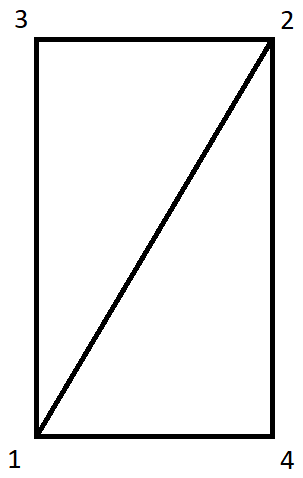
\includegraphics[width=0.25\textwidth]{kepek/billboardFrame.png}
 \caption{A billboard váza a csúcspontokkal.}
 \label{fig:spriteFrame}
\end{wrapfigure}

Minden VBO-hoz meg kell határozni, hogy az abban tárolt adatokat a shader program melyik attribútumán keresztül kapja meg. Mivel ezek az attribútumok alapértelmezetten le vannak tiltva, először külön engedélyezni kell őket. 

%calculateSpriteVertices()
A pontok meghatározását a \texttt{calculateSpriteVertices} metódus végzi. A textúrán 4 sorban és 8 oszlopban helyezkednek el rajta az állapotok, tehát egy állapot oldalainak aránya 2:1. Ez azt jelenti hogy a megjelenítésnél egy téglalapra kell ráhúzni képeket. A téglalapot természetesen 2 háromszög alkotja, amint az az \ref{fig:spriteFrame}. ábrán is látszik. 
Mivel az alakzatot az $Y$ tengely körül kell majd a későbbiekben forgatni, érdemes úgy definiálni a pontokat, hogy a téglalap alsó élének középpontja az origóba essen, hogy az a forgatás során egy helyben maradjon. A téglalap síkja pedig az $XY$ síkkal esik majd egybe, mert így egyszerűbb definiálni. Konkrét koordinátákkal is meghatározhatnám a téglalapot, de akkor minden kirajzolás esetén a modellmátrixot a skála paraméternek megfelelően skálázni kell. Hogy ezt a műveletet megspóroljam, eleve a skála segítségével határozom meg a koordinátákat. Az $Y$ koordináták a 0 vagy a skála értékét veszik fel, az $X$ koordináták azonban a $\pm \frac{\text{skála paraméter}}{4}$ értékeket, hiszen a magasság felét még az origó is kettéosztja. A pontokat az óramutató járásának irányával ellentétes sorrendben érdemes megadni, hogy a későbbiekben szükség esetén könnyen lehessen belőlük normálvektort számítani. Így tehát az első háromszög pontjai az 1, 2, 3 pontok, a másodikéi pedig 1, 4, 2. A pontokat ebben a sorrendben kell tárolni, ehhez mindig a C++ standard könyvtárának vektor típusú tárolóját használom, ugyanis kezelése könnyű, dinamikus a mérete és felszabadítja a lefoglalt helyet maga után.

%calculateNextTextureCoordinates()
Az ezekhez a pontokhoz tartozó textúra koordinátákat a \texttt{calculateNextTextureCoordinates} metódussal állítom elő. Mivel egy képen van több állapotom, ezek az értékek állapotról állapotra változnak. Egy adattag (\texttt{m\_iActualFrame}) segítségével számon tartom, hogy éppen hányadik állapotnál járok, és ebből a számból határozom meg a hozzá tartozó koordinátákat. A számozást 0-tól kezdem. Először a sor és oszlopszámot kell kiszámolni hozzá. A sort az $\frac{\text{állapot sorszáma}}{\text{oszlopok száma}}$ hányados egész része adja meg, az oszlopot pedig az előbbi osztás maradéka (modulo művelet). A textúra koordináták a bal felső sarokból $(0, 0)$ indulnak, és a jobb alsó sarok $(1, 1)$ felé nőnek. Az adattagok között számon tartom, hogy egy állapot a textúra koordináta-rendszernek megfelelően milyen széles (\texttt{m\_fColumnstep}), és milyen magas (m\_fRowstep). Ennek megfelelően például az állapot bal felső pontjának $(u, v)$ koordinátája az 
\begin{align*}
u &= \text{adott oszlop} \cdot \text{szélesség}, \\
v &= \text{adott sor} \cdot \text{magasság}, 
\end{align*}
a jobb alsó pedig az  
\begin{align*}
u &= (\text{adott oszlop} + 1) \cdot \text{szélesség}, \\
v &= (\text{adott sor} + 1) \cdot \text{magasság} 
\end{align*}
egyenletek alapján kapható meg. Az így kapott $(u, v)$ koordinátákat a téglalap objektum pontjainak megfelelő sorrendben kell megadni, azaz 1, 2, 3, 1, 4, 2, ahol például 1 a bal alsó, 2 a jobb felső ponthoz tartozó koordináták. A metódus utolsó lépéseként növeljük az állapot sorszámát tároló adattag értékét eggyel, ügyelve arra, hogy az utolsó állapotot követően nullázzuk.

%VAO generálás
Ezek után generálunk egy VAO-t és a két vektort, melyeket az előbbi funkciókkal állítottunk elő, külön-külön VBO-k segítségével tároljuk a VAO-ban. A két VBO között fontos különbség, hogy amíg a pontokat statikus objektumként tároljuk le, addig a textúra koordinátákat dinamikusként kell, ugyanis ennek a VBO-nak a tartalma fog változni az animáció során. Ezt a \texttt{GL\_DYNAMIC\_DRAW} paraméter segítségével jelezhetjük a grafikus processzornak, amely így ennek megfelelően allokálja a puffer számára a helyet, például a saját memóriája helyett akár a gép memóriáját is használhatja.
A VBO generálás a következőképpen néz ki:
\begin{cpp}
glGenBuffers(1, &m_iFireVBO);
glBindBuffer(GL_ARRAY_BUFFER, m_iFireVBO);
glBufferData(GL_ARRAY_BUFFER, 
	textureCoordinates.size() * sizeof(glm::vec2), 
	&textureCoordinates.front(), GL_DYNAMIC_DRAW);
glEnableVertexAttribArray(m_pFireShader->attrib("vertTexCoord"));
glVertexAttribPointer(m_pFireShader->attrib("vertTexCoord"), 2, 
	GL_FLOAT, GL_FALSE, 0, NULL);
\end{cpp}
A \texttt{glGenBuffers} generál egy VBO-t és az azonosítóját beírja a második paramétereként megadott helyre, melyet a \texttt{glBindBuffer}-nek átadva ``használatba helyezhetjük'' (bind-eljük) a puffert. A \texttt{glBufferData} függvénnyel definiálhatjuk a puffer tartalmát, jelen esetben a textúra koordinátákat tároljuk majd benne. Az első paramétere megadja a puffer fajtáját, itt most pontok tulajdonságára utaló adatokkal lesz feltöltve. A második paraméter a másolni kívánt adat méretét adja meg, a harmadik pedig a tároló objektum kezdőcímét. Az utolsó paraméter a VBO használatára utal. A példában \texttt{GL\_DYNAMIC\_DRAW} mellett még a \texttt{GL\_STATIC\_DRAW} konstanst használtam még az olyan a VBO-k esetén, melyek tartalmát nem változtatom. A \texttt{glEnableVertexAttribArray} függvény engedélyezi a megadott attribútum használatát a shader programban, a \texttt{glVertexAttribPointer} pedig megadja, hogy az adott VBO-t melyik attribútumon keresztül kapja meg a shader. Utóbbi függvény második paramétere adja meg, hogy hány komponensből áll egy csúcspont tulajdonság, ezt követi a komponensek típusa. A negyedik paraméter megadja, hogy az egész értékű adattípusokat normalizálja-e, vagy sem. Az utolsó előtti paraméter adja meg a pont tulajdonságok közti offset-et, végül pedig a pufferben az első tulajdonság előtti offset-et adjuk meg.

A \texttt{loadVAO} metódus tehát betöltött minden szükséges adatot, amely a kirajzoláshoz szükséges.

% DRAW
A kirajzolást a \texttt{drawFire} metódus végzi. Először be kell állítani a használni kívánt shader-t, majd bind-elni kell a használni kívánt textúrát. Ezt át is kell adni a shader-nek, esetemben a tex uniform-on keresztül. Ezt követően bind-eljük a VAO-t, amelyben a pontok adatait tároljuk. Ha csupán egy sprite-ot szeretnénk kirajzolni, akkor megadjuk a shader-nek a modell mátrixot (amely az eltolást és az esetleges forgatást végzi el a pontokon), majd a \texttt{glDrawArrays} segítségével kirajzoljuk a háromszögeket. Ha szeretnénk 90 fokkal elforgatva is kirajzolni a sprite-ot, akkor a modell mátrixot még 90 fokkal elforgatjuk a GLM könyvtár \texttt{rotate} metódusának segítségével, ezt ismét átadjuk a shader-nek, eztán pedig megint kirajzoljuk a VAO-t. Az átlátszóság kezelése miatt itt már a sorrendre is figyelni kell, de ezt is a későbbiekben fejtem majd ki. A rajzolások után kikapcsoljuk az adott VAO, textúra és shader használatát. A \texttt{drawFire} metódus végén az \texttt{m\_fElapsedTime} adattaghoz hozzáadjuk az előző kirajzolás óta eltelt időt, melyet a camera objektumtól kérdezhetünk le. Ebben az adattagban számoljuk az előző állapotváltás óta eltelt időt. Amennyiben ez átlépi a határt (\texttt{m\_fAnimationSpeed}), a következő állapot textúra koordinátáit kell betöltenünk. Ehhez bind-elni kell az adott VBO-t, majd a \texttt{calculateNextTextureCoordinates} metódus segítségével előállítani a megfelelő textúra koordinátákat. A puffer tartalmát a \texttt{glBufferSubData} függvény segítségével írhatjuk át. Ezzel a puffer tartalmának egy részét is át lehetne írni, de nekem az egészet át kell. Ennek ellenére is hatásosabb ezt használni a \texttt{glBufferData} helyett, ugyanis így a szükséges memória újraallokálását el lehet kerülni. Végül nullázzuk az \texttt{m\_fElapsedTime} adattagot.

% shaderek
% TODO: Helyes ez így?
A vertex és fragmet shaderek itt rendkívül egyszerűek. A vertex shader csak a csúcspontokat és a textúra koordinátákat kapja meg a szükséges transzformációs mátrixok mellett. A pontokat továbbadja a fragment shader-nek, a pozíciót (\texttt{gl\_Position}) pedig a kamera és modell mátrixokkal megszorzott, homogén koordinátával kibővített csúcspont helye adja meg. A fragment shader pedig a uniform-ként kapott textúrából a textúra koordináta alapján kiolvasott értéket adja meg a pixel színeként. 

% TODO: Az osztályok bemutatása így kicsit sűrű. Néhány UML félével lehetne rajta szinesíteni.

\subsection{BillboardFire osztály}

A billboard tűzhöz külön osztályt készítettem. A \texttt{BillboardFire} osztály egyik adattagja \texttt{SpriteFire} típusú, hiszen abban már implementálva van az egyszerű 1 téglalapon alapuló megjelenítés is. A \texttt{BillboardFire} konstruktorának szüksége van a tűzhöz használt shader program, a camera objektum és a tűz megjelenítési pozíciójára is. A skála paraméter itt is opcionális. Ezen paraméterek segítségével inicializálom a \texttt{SpriteFire} adattagot úgy, hogy csak egy felületet rajzoljon ki. 

A sprite tűzhöz képest tehát annyi a különbség, hogy az objektum mindig a kamerával szembe fordulva van kirajzolva. A \texttt{drawFire} metódus itt csak beállítja a \texttt{SpriteFire} adattag elfordulását a \texttt{setRotation} metódusával, majd meghívja annak a \texttt{drawFire} metódusát. Az elfordulást a \texttt{calculateRotation} metódus állapítja meg:
\begin{cpp}
float angle = 0.f;
glm::vec2 cameraPos(m_pCamera->getX(), m_pCamera->getZ());
glm::vec2 firePos(m_vPosition.x, m_vPosition.z);

glm::vec2 eye = glm::normalize(cameraPos - firePos);

float cosAlpha = glm::dot(eye, glm::vec2(0.f, -1.f)); 

if (cameraPos.x < firePos.x)
{
	angle = glm::acos(cosAlpha);
}
else
{
	angle = glm::acos(-cosAlpha);
}

return angle;
\end{cpp}
Mivel a tűz alap esetben a $-Z$ tengely felé néz, ehhez a tengelyhez kell mérni az elfordulást is. Ehhez szükség van a kamera és a tűz $XZ$ sík menti pozícióira (\texttt{cameraPos}, \texttt{firePos}). Az \texttt{eye} vektor a tűz pozíciójából a kamera pozíciójába bocsátott vektor. Az $\bar{a}$ és $\bar{b}$ vektor által bezárt szög koszinuszát a következő egyenlet alapján kaphatjuk meg: 
$$
\cos \alpha = \frac{\bar{a} \cdot \bar{b}}{|\bar{a}| \cdot |\bar{b}|}
$$
% TODO: Nyomtatásban félkövérrel szokták jelölni inkább a vektorokat.

Amennyiben a két vektor normalizált, azaz a hosszuk egységnyi hosszú, az egyenletben az osztó értéke 1, tehát azt el is hagyhatjuk, ha normalizált vektorokkal számolunk. Ezért a \texttt{cosAlpha} változó értékéhez elég a két vektor (\texttt{eye} és $-Z$) skaláris szorzatát venni. Mivel a két vektor által bezárt szög definíció szerint kisebb, vagy egyenlő, mint 180$^{\circ}$, a két pozíció $X$ tengely menti helyzetéhez viszonyítva el kell dönteni, hogy mikor kell a szög -1-szeresével számolni. 

% átlátszóság
\subsection{Az átlátszóság kezelése}

Ha a tűz állapotait tároló képen csak teljesen áttetsző, és teljesen átlátszatlan pixelek lennének, akkor az átlátszóságot egy egyszerű OpenGL-es alfa teszt funkció segítségével meg lehetne oldani. Ez a neki megadott paraméterek alapján bizonyos alfa értékek felett (vagy alatt) kirajzolja az adott pixelt, egyébként nem. Színkeverést tehát nem végez, így kicsivel gyorsabb is, mint a blending funkciók.

Az általam letöltött textúra azonban az alfa csatorna teljes skáláját kihasználja, így muszáj valamilyen blending funkciót használni. A blending az OpenGL-ben a fragment shader kimeneti színét (forrás szín) keveri a színpufferben a megfelelő helyen található színnel (cél szín). Ennek működése két, paraméterekkel befolyásolható függvény segítségével adható meg. Mindenek előtt a \texttt{glEnable(GL\_BLEND)} parancs segítségével engedélyezni kell a blending-et.

A \texttt{glBlendEquationSeparate(GLenum modeRGB, GLenum modeAlpha)} függvény határozza meg a keveréskor elvégzendő alapműveletet külön az RGB komponenseken, és külön az alfa csatornán. Az én esetemben a forrás és a cél színeket össze kell majd adni, így mindkét paraméternek a \texttt{GL\_FUNC\_ADD} konstanst kell átadni.

A \texttt{glBlendFuncSeparate(GLenum srcRGB, GLenum dstRGB, GLenum srcAlpha,\\ GLenum dstAlpha)} függvény segítségével adhatjuk meg, hogy mely komponenseket mivel szorozzuk meg az összeadás előtt. Az első két paraméter a forrás és a cél RGB komponenseire utal, az utolsó kettő pedig ezek alfa csatornáira, így a kimeneti színt a következőképpen kaphatjuk meg: 
\begin{align*}
\text{OutputRGB} &= \texttt{srcRGB} \cdot \text{forrásRGB} + \texttt{dstRGB} \cdot \text{célRGB}, \\
\text{OutputAlfa} &= \texttt{srcAlpha} \cdot \text{forrásAlfa} + \texttt{dstAlpha} \cdot \text{célAlfa}.
\end{align*}
A cél a tűz megjelenítése során, hogy a tűz pixelének a színe a saját (forrás) alfa komponensével legyen megszorozva, és hogy a $[0, 1]$ tartományon belül maradjon a kimeneti érték, a háttérszínt (cél) az 1 - forrás alfa komponenssel szorozzuk meg. Az alfa csatornák értéke ebben az esetben nem játszik sok szerepet, így a hagyományos blending-nek megfelelően a forrás alfa értéke lesz a kimeneti alfa is. A két függvény tehát a következőképpen fog kinézni:
\begin{cpp}
glBlendEquationSeparate(GL_FUNC_ADD, GL_FUNC_ADD);
glBlendFuncSeparate(GL_SRC_ALPHA, GL_ONE_MINUS_SRC_ALPHA,
	 GL_ZERO, GL_ONE);
\end{cpp}

% Kitakarás
\begin{figure}[h]
 \centering
 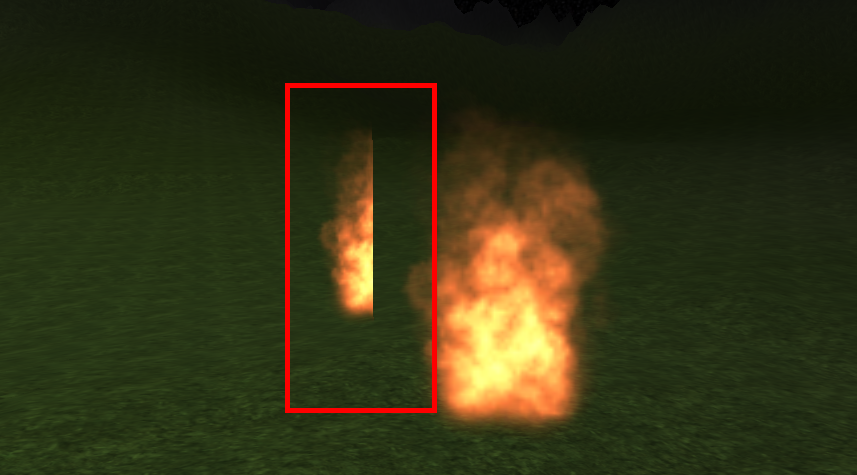
\includegraphics[width=\textwidth]{kepek/billboardOverlap.png}
 \caption{Kitakarás a blending után}
 \label{fig:spriteOverlap}
\end{figure}
\begin{figure}[h!]
 \centering
 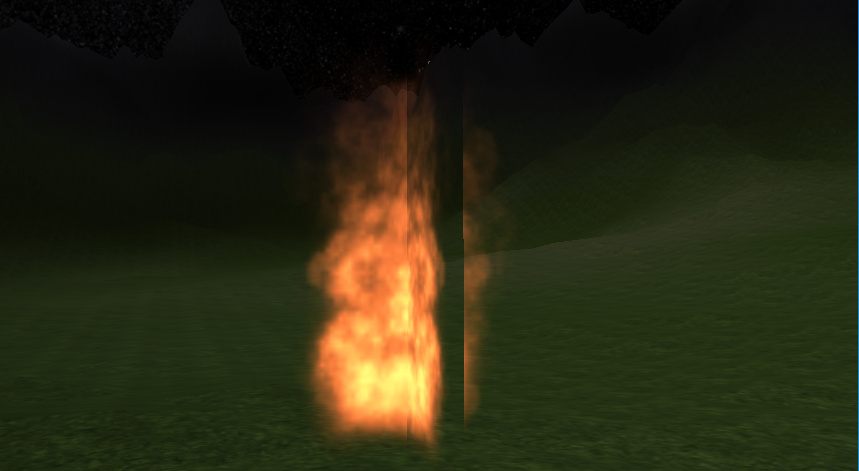
\includegraphics[width=\textwidth]{kepek/doubleBillboard1.png}
 \caption{2 síkból álló sprite probléma}
 \label{fig:doubleSprite}
\end{figure}

Így már egészen valósághű eredményt kapunk. Azonban mikor a színpuffert írjuk, gondoskodni kell róla, hogy abban már minden, a tűz hátterében feltűnő objektum színe jelen legyen.

 Ha ugyanis valamely objektum még nem került kirajzolásra a háttér elemek közül, akkor a sprite teljesen áttetsző részein sem fog szerepelni, így egy része lehet hogy átlátszósággal lesz kitakarva. Ezt figyelhetjük meg \aref{fig:spriteOverlap}. ábrán is, ahol a közelebbi sprite korábban kerül kirajzolásra, mint a mögötte lévő. A kirajzolandó objektumokat ezért a kamerától mért távolságuk alapján csökkenő sorrendben kell kirajzolni, azaz a legtávolabbiakkal kell kezdeni. Ezzel az egyszerűbb esetek meg is vannak oldva, azonban ha két objektum keresztezi egymást, mint például a 2 síkból álló billboard (\ref{fig:doubleSprite}. ábra), akkor nincs olyan kirajzolási sorrend, amely kiküszöbölné a kitakarást.

Az egyik megoldás, hogy valamelyik síkot két részre kell bontani a közepénél, így lesz 3 különböző objektum, melyeket már könnyebben sorba lehet rendezni. Hogy a \texttt{BillboardFire} osztály működését ne befolyásoljam, a \texttt{SpriteFire} osztályban a második, elforgatott sík nem az eredeti újrakirajzolásából áll majd elő, hanem egy új VAO-t hozok létre erre a célra, melyet majd két részletben rajzolok ki. Hogy ne kelljen külön forgatni, eleve az $YZ$ síkkal lesz párhuzamos. 

\begin{figure}[h]
 \centering
 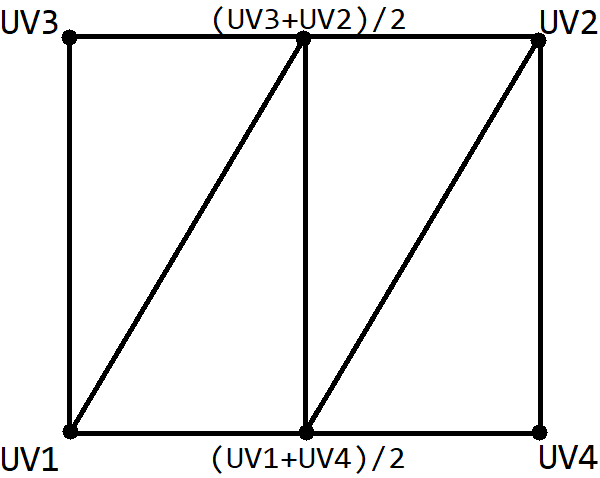
\includegraphics[width=0.5\textwidth]{kepek/billboardUVcoords.png}
 \caption{$(u, v)$ koordináták az Y tengely mentén}
 \label{fig:spriteUVcoords}
\end{figure}

A \texttt{calculateSpriteVertices} metódust kibővítettem, hogy amennyiben 2 síkot kell kirajzolni, a további 12 pontot (két külön sprite) is csatolja a visszatérési tárolóba. A pontok sorrendje itt is pontosan úgy van megadva, ahogyan az az eredeti síkon van (\ref{fig:spriteFrame}. ábra). 

A \texttt{calculateNextTextureCoordinates} metódust is hasonlóképpen egészítettem ki. Itt azonban a két sík találkozásánál található pontok textúra koordinátáit más módszerrel kellett meghatározni, mint alap esetben.
A megoldást az adott ponttal egy magasságban lévő textúra koordináták közti lineáris interpoláció jelentette, ahogyan az \aref{fig:spriteUVcoords}. ábrán is látszik. Ezt a 12 pontot szintén a vektor gyűjteményhez csatolja, mellyel visszatér.

Tehát ha kétsíkú sprite-ot kell kirajzolni, akkor a \texttt{loadVAO} metódusban a \texttt{vertices} és a \texttt{textureCoordinates} változók már 6 helyett 18 elemből állnak, melyekből két külön VAO-t kell készíteni. Az eredeti sík VAO-jában csak annyi változás történik, hogy a \texttt{glBufferData} függvény méretre vonatkozó paraméterét nem a vektor gyűjtemény méretéből számoljuk ki, hanem megadjuk, hogy 6-szor kell venni a gyűjtemény egy elemének méretét. Így csupán az első 6 elem kerül bele, ahogy az eddig is történt. A második VAO-t ehhez hasonlóan hozzuk létre, ám a \texttt{glBufferData} második (méret) és harmadik (az első elem pointere) paraméterében meg kell adni, hogy 12 elemet tároljon le a puffer 6-os indexű elemétől kezdve. Ez a csúcspontok VBO-ja esetén a következőképpen néz ki:
\begin{cpp}
glBufferData(GL_ARRAY_BUFFER, 12 * sizeof(glm::vec3), 
	&vertices[6], GL_STATIC_DRAW);
\end{cpp}

A \texttt{drawFire} metódus mellé segédmetódusoknak külön elkészítettem a \texttt{drawNormalVAO}, \texttt{drawSecondary1VAO} és \texttt{drawSecondary2VAO} metódusokat. Az első az eredeti síkot rajzolja ki, a második a (szemből nézve) bal oldali ``fél'' sprite-ot, a harmadik pedig a jobb oldalit. Ezekben csupán a VAO bindelés, valamint a \texttt{glDrawArrays} hívás található. A másodlagos (secondary) kirajzoló függvények között csupán a \texttt{glDrawArrays} hívás különbözik, az első ugyanis az első 6 elemét, a második pedig a VAO második 6 elemét rajzolja ki (\texttt{glDrawArrays(GL\_TRIANGLES, 6, 6)}). 

\begin{figure}[h]
 \centering
 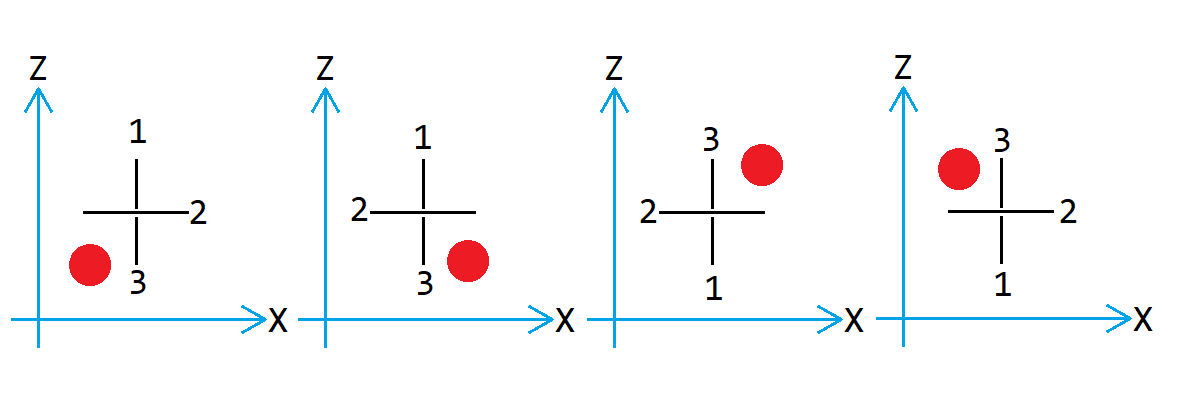
\includegraphics[width=\textwidth]{kepek/billboardSorting.png}
 \caption{Kirajzolási sorrend a ``kétsíkú'' sprite estén}
 \label{fig:spriteSorting}
\end{figure}
A kirajzoláskor a \ref{fig:spriteSorting}. ábrán látható esetek fordulhatnak elő. A piros folt a kamera helyzete, a fekete kereszt a tűz 3 külön kirajzolt sprite-ját jelképezi. A blending kedvéért a kamerától legtávolabb eső objektumokkal kell kezdeni. A renderelés sorrendjét a számok jelzik. Ez alapján jól látszik, hogy esetemben a kamera és a tűz pozíciójának $Z$ koordinátáit kell csupán összevetni, és ezek alapján két különböző kirajzolási sorrend lehetséges. 
Például az első eset (bal szélső kettő) kirajzolása: 
\begin{cpp}
if (m_pCamera->getZ() < m_vPosition.z)
{
	drawSecondary2VAO();
	drawNormalVAO();
	drawSecondary1VAO();
}
\end{cpp}
Így már kirajzoláskor minden nézőpontból helyes képet kapunk.

Ha egymás mellé kirajzolunk egy billboard és egy kétsíkú sprite objektumot, akkor \aref{fig:billboardFinal1}. ábrán látható eredményt kapjuk.

\begin{figure}[h!]
 \centering
 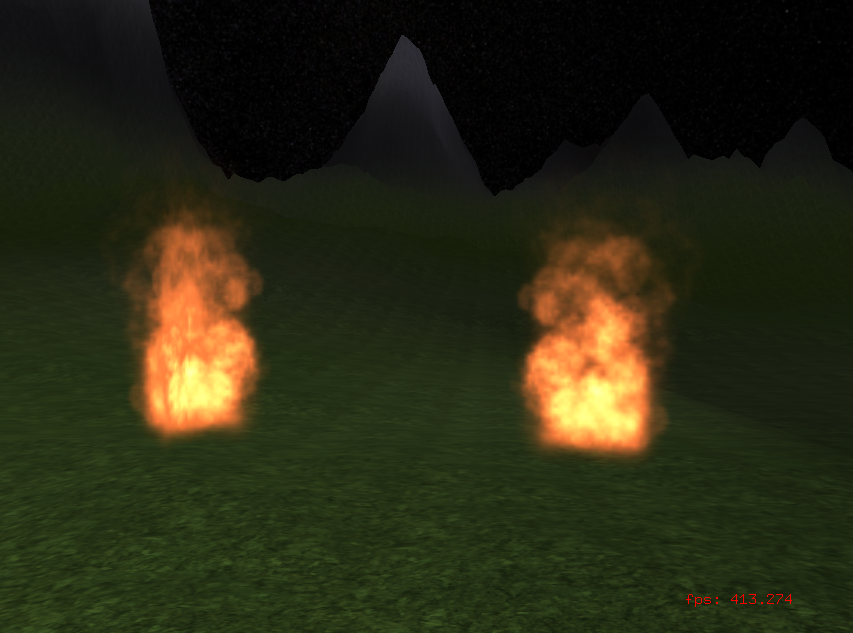
\includegraphics[width=0.95\textwidth]{kepek/billboardFinal1.png}
 \caption{Bal oldalon a kétsíkú sprite, jobb oldalon a billboard látszik.}
 \label{fig:billboardFinal1}
\end{figure}

\Aref{fig:billboardFinal2}. ábrán megfigyelhetjük, hogy a helyes sorrendbeli kirajzolásnak köszönhetően a blending szép kitakarást eredményez minden irányból.

\begin{figure}[h!]
 \centering
 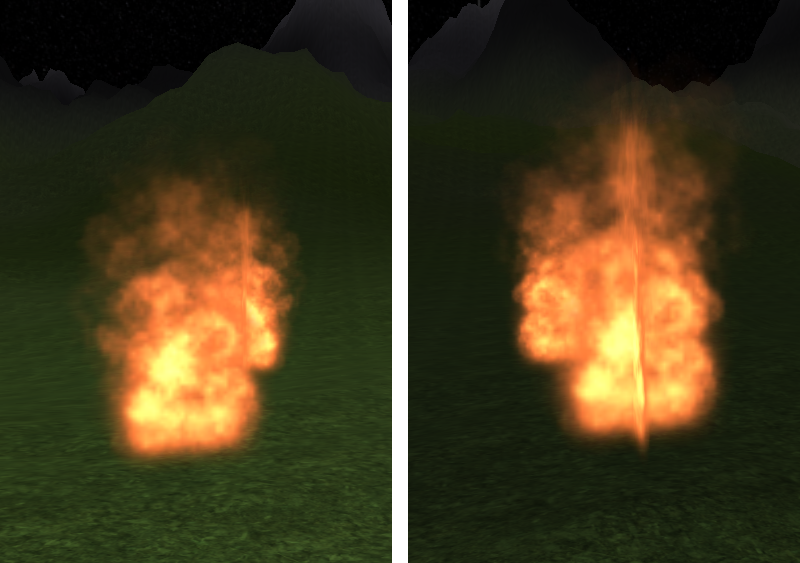
\includegraphics[width=0.85\textwidth]{kepek/billboardFinal2.png}
 \caption{Bal oldalon a billboard takar ki, jobb oldalon pedig a sprite}
 \label{fig:billboardFinal2}
\end{figure}

\Aref{fig:billboardFinal3}. ábrán mutatkozik a kétsíkú sprite egyik gyengesége. Ha ugyanazt a textúrasorozatot használjuk fel, akkor bizonyos szögekből a kép ugyanazon fele kerül egymással szembe, mely feltűnő lehet. Erre egy megoldás lehet a második síkra egy külön textúra sorozat készítése.

\begin{figure}[h!]
 \centering
 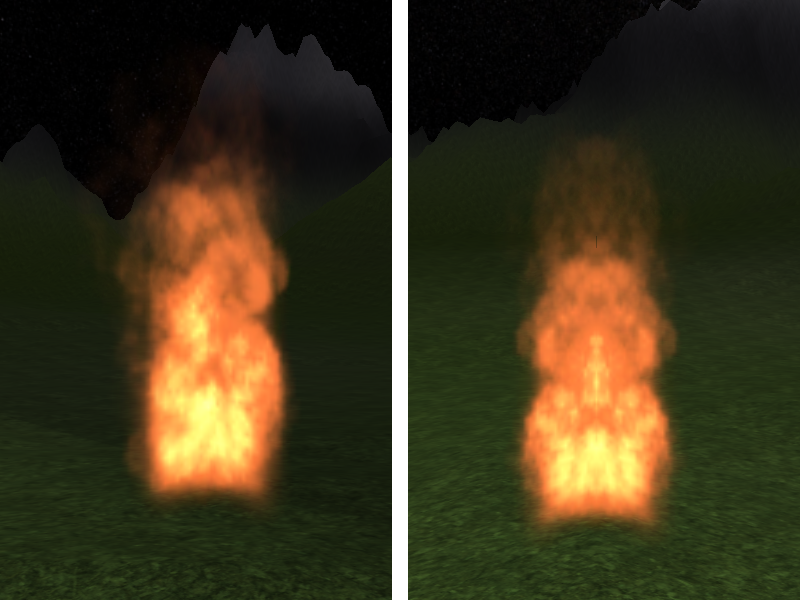
\includegraphics[width=0.85\textwidth]{kepek/billboardFinal3.png}
 \caption{A bal oldali kép esztétikusabb, a jobb oldalin feltűnő a tükröződés}
 \label{fig:billboardFinal3}
\end{figure}

\Aref{fig:billboardFinal4}. ábrán pedig megfigyelhető a kétsíkú sprite másik gyenge pontja. Ha valamelyik síkra nagy szögben tekintünk, akkor feltűnővé válhat a körvonala, rombolva ezzel a látványt.

\begin{figure}[h!]
 \centering
 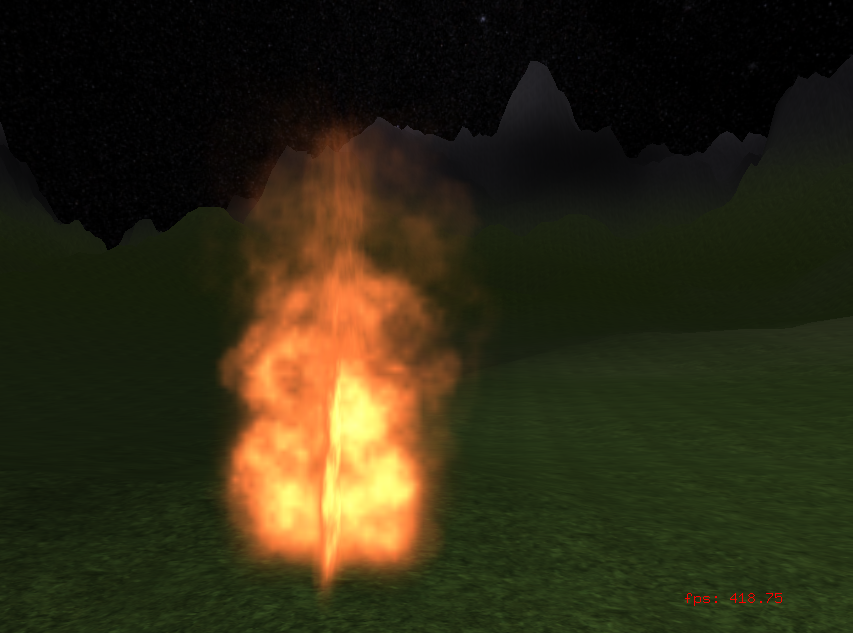
\includegraphics[width=0.85\textwidth]{kepek/billboardFinal4.png}
 \caption{Mozgás közben még szembetűnőbb a körvonal}
 \label{fig:billboardFinal4}
\end{figure}

\Aref{fig:billboardFinal5}. ábrán enyhe felülnézetből látszik igazán a két megjelenítési mód közötti különbség. Ebből a perspektívából egyik sem szerepel túl jól.

\begin{figure}[h!]
 \centering
 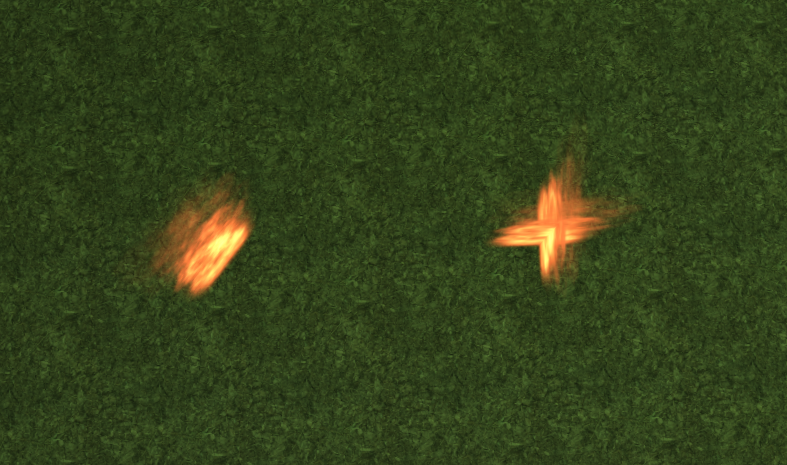
\includegraphics[width=0.85\textwidth]{kepek/billboardFinal5.png}
 \caption{Bal oldalon a billboard, jobb oldalon a sprite tűz}
 \label{fig:billboardFinal5}
\end{figure}
% Videón körbejárás, és a sebesség paraméter hatása

% fps, pontok száma, 
\subsection{Számításigény}
A másodpercenként kirajzolt képek számát egy billboard és egy 2 síkú sprite tűz nem befolyásolja, hiszen komolyabb számítást nem kell végeznie a gépnek, összesen csupán $6 \cdot 4 = 24$ pontot kell kirajzolni.


%%%%%%%%%%%%%%%%%%%%%%%%%%%%%%%%%%%%%%%%%%%%%%%
\section{Háromdimenziós részecskerendszer alapú tűz}

% FireParticle class
\subsection{FireParticle osztály}

A részecskerendszer alapú tűz részecskéinek implementálásakor a billboard alapú megjelenítést választottam váltogatott textúrával, ugyanis ezzel tudtam jelenleg a legvalószerűbb hatást elérni. Az osztályra nagyrészt egy adott részecske tulajdonságainak és helyzetének a tárolása végett volt szükség. Emellett ez végzi el képkockánként egy részecske élettartamának, pozíciójának, sebességének, méretének, elfordulásának és textúrájának a frissítését. A modell heurisztikus alapokon nyugszik, a tűz fizikai tulajdonságait utánozni próbálva. A kirajzolás nem ebben az osztályban történik.

% főbb adattagok 
\subsubsection{Adattagok}
A részecskéket a következő fontosabb tulajdonságokkal vérteztem fel:
\begin{itemize}
\item Élettartam és kor (\texttt{m\_fLifeTime}, \texttt{m\_fAge}): a kor kezdetben az élettartammal egyenlő, majd folyamatosan csökken $0$-ig.
\item Pozíció, mozgás irány, sebesség (\texttt{m\_vPosition}, \texttt{m\_vSpeedDirection}, \texttt{m\_fSpeedRate}): az irány nem egységvektor, így még nagyobb és véletlenszerűbb a különbség a részecskék mozgása között.
\item Méret és növekedési ráta (\texttt{m\_fScale}, \texttt{m\_fScaleRate}): a növekedési ráta adja meg a részecske, mint gáz tágulásának a sebességét.
\item A kamerától vett távolság (\texttt{m\_fDistanceToCamera}): ez alapján lesznek majd sorba rendezve a részecskék.
\item $Z$ tengely menti elfordulás és szögsebesség (\texttt{m\_fRotation}, \texttt{m\_fRotationRate}): ezek segítségével keltek turbulens hatást az animáció során.
\item Textúrák száma, pillanatnyi textúra sorszáma (\texttt{m\_cNumberOfTextures}, \\ \texttt{m\_cCurrentTexture}): a textúrák számozása $0$-tól indul.
\item A láng és füst állapotok aránya, a pillanatnyi keverés aránya, egy jelenet ideje (\texttt{m\_fFireTimeRatio}, \texttt{m\_fCurrentBlend}, \texttt{m\_fSceneTime}): a későbbiekben kerülnek kifejtésre.
\end{itemize}

% konstruktor
\subsubsection{Konstruktor}
Az osztály konstruktora paraméterként várja az adott részecske indulási pozícióját, a sebességének irányát, az elfordulását, az élettartamát, a forgás szögsebességét, a részecske sebességét, illetve egy, a \texttt{Camera} osztály példányára mutató pointert. Ezeket lementi a megfelelő adattagokba, illetve kiszámol néhány további származtatott adatot. 

Ilyen az \texttt{m\_fSceneTime} adattag is, mely megadja, hogy a textúra sorozat egyes tagjai (melyek váltogatása a részecske animációját eredményezi) hány milliszekundumot (a továbbiakban \textit{ms}) szerepelnek. Ezt a textúrán szereplő állapotok száma és a részecske élettartamának a hányadosa adja meg. 

A füsthöz nem készítettem külön emittert és osztályt. Egy részecske az életének egy bizonyos részét lángként, utána pedig füstként tölti. A füsthöz nem alkalmaztam külön textúrát, hanem a láng képsorozat utolsó tagját használtam fel kiszürkítve. Ebből következik, hogy az \texttt{m\_fSceneTime} adattagot még meg kell szorozni az \texttt{m\_fFireTimeRatio} adattaggal. Ez a $[0, 1]$ tartományon értelmezett szám adja meg, hogy a részecske az életének hányad részét tölti láng fázisban. Egy állapot tehát rövidebb ideig szerepel majd, de az utolsó jelenetet leszámítva mind ugyanannyi időt töltenek majd a képernyőn. 

% update
\subsubsection{Részecskék állapotának frissítése}
Az \texttt{update} metódus felel a részecskék karbantartásáért. A metódusnak paraméterként meg kell adni az előző frissítés óta eltelt időt ms-ban (\texttt{elapsedTime}). Ezzel első lépésként csökkentjük a részecske korát, majd megvizsgáljuk, hogy életben van-e még ($\texttt{m\_fAge} > 0$). Ha nem, akkor a függvény hamis értékkel tér vissza, ha igen, akkor frissíti az adattagokat, majd igaz értéket ad vissza. A frissítéshez két segédváltozó szükséges: a lépték és a részecske relatív kora (\texttt{step}, \texttt{relativeAge}). A léptéket az eltelt idő század részének választottam meg, a relatív kor pedig a részecske korának és élettartamának hányadosa, azaz 1-től indul és végül 0-hoz ér el. Az adattagokat a következők alapján módosítottam: 
\begin{cpp}
// Slowing x and z much faster than y
m_vSpeedDirection.x /= 1.f + step * 0.05f * relativeAge;
m_vSpeedDirection.z /= 1.f + step * 0.05f * relativeAge;
m_fSpeedRate /= 1.f + step * 0.01 * (1-relativeAge);

// Extra forces
if (m_bForceApplied)
{
	m_vPosition += m_vForceDirection * m_fForceSpeed * step;
	m_bForceApplied = false;
}

// Moving
m_vPosition += m_vSpeedDirection * step * m_fSpeedRate;

// Expanding
m_fScale += m_fScaleRate * step;

// Rotate
m_fRotation += step * m_fRotationRate;

// Changing texture
{...}

m_fDistanceToCamera = glm::distance2(
		m_vPosition, m_pCamera->getPosition());
\end{cpp}
A lépték változóval történő szorzás a korábbiakban tárgyalt okokból történik, hogy az adattagok az eltelt idő függvényében változzanak. A relatív életkorral történő szorzás pedig olyan esetekben volt szükséges, mikor a változást a részecske korától is függővé kellett tenni.

A sebesség irányának $x$ és $z$ koordinátáit azért kellett nagyobb mértékben csökkenteni, hogy a részecskék ne egyenes vonalban távolodjanak egymástól, mint például egy robbanás esetén, hanem parabolaszerűen egyre függőlegesebben emelkedjenek (\ref{fig:parabolicSpeedVector}. ábra). A részecske korának csökkenésével (azaz az öregedésével) egyre kisebb mértékű a csillapítás is.
\begin{figure}[h]
 \centering
 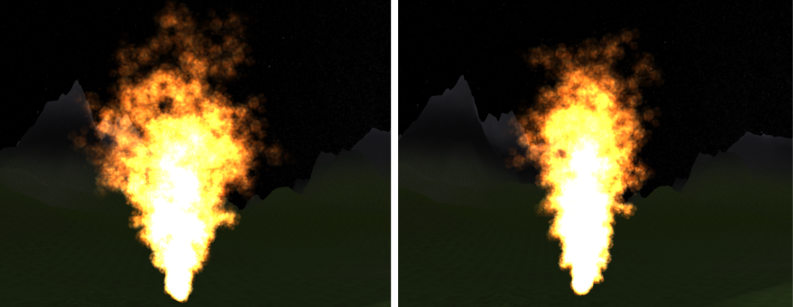
\includegraphics[width=\textwidth]{kepek/parabolicSpeedVector.png}
 \caption{Bal oldalon a csillapítás nélküli, jobb oldalon a lassított $x$ és $z$ koordinátákkal kapott eredmény.}
 \label{fig:parabolicSpeedVector}
\end{figure}
A részecskék sebességét viszont annál jobban csökkentettem, minél közelebb ér élete végéhez. 

A külső erőket egy publikus metódus (\texttt{applyForce(glm::vec3 direction, float speed)}) segítségével lehet hozzáadni, ám ezt minden frissítés előtt meg kell tenni. Ez azért alakult így, mert a külső erőket más osztályok szabályozzák, de képkockáról képkockára változhatnak azok is. A megadott irányba a megadott sebességgel hatok a részecske pozíciójára a frissítés során.

A kamerától vett távolság kiszámításakor a négyzetes távolságot veszem (\texttt{glm::dis\-tance2}), így egy gyökvonást megspórolok, de a végső sorrenden ez úgysem változtat. A mozgatás, tágulás és forgatás nem igényelnek különösebb magyarázatot.

%textúrázás
\subsubsection{Textúrázás}
A textúrázás a billboard alapú tűznél alkalmazott módszerre hasonlít. Mivel a textúra koordinátákat minden részecskére ki kell számolni, és egyszerre két jelenet koordinátáira is szükség van, részecskénként $6 \cdot 4 = 24$ db \texttt{float} koordinátát kellene átküldeni (és a lassú CPU-n kiszámolni) az árnyalónak. Mivel egyébként is sok információt kell nekik eljuttatni, és az adatmozgatás a shader-ek felé aránylag lassú művelet, inkább a vertex shader-ben végzem a koordináták meghatározását. Ahhoz, hogy ott el tudjam végezni a műveletet szükség van azonban a pillanatnyi textúra sorszámára. Ennek meghatározása során oda kell figyelni arra is, hogy a részecske láng, vagy füst fázisban van-e.

\begin{cpp}
// Changing texture
float textureInfo = (m_fLifeTime - m_fAge) / m_fSceneTime;
m_cCurrentTexture = (int)textureInfo;
if (m_cCurrentTexture < m_cNumberOfTextures)
{
	// Flame
	m_fCurrentBlend = 1.f - fmod(textureInfo, 1.0f);
}
else
{
	// Smoke
	m_cCurrentTexture = m_cNumberOfTextures;
	// fade the somke out
	m_fCurrentBlend = relativeAge / (1 - m_fFireTimeRatio);
	m_fScale += 0.1 *step;
}
\end{cpp}

A \texttt{textureInfo} segédváltozóban kiszámolom, hogy a születés óta eltelt idő alatt hányszor telt el az egy jelenetre jutó idő. Ennek az egész része adja meg a pillanatnyi textúra sorszámát (\texttt{m\_cCurrentTexture}). Ha ez a szám nem kisebb, mint a textúrák száma, az azt jelenti hogy a részecske már a füst fázisban tart.

Hogy az animáció még folyékonyabb legyen a láng fázisban, egyszerre két jelenetet használok fel a textúrán található képsorozatból: a pillanatnyi textúrát, és az utána következőt. Ezt a kettőt mosom össze annak alapján, hogy a pillanatnyi textúrára jutó időből mennyi van még hátra. Az ehhez szükséges arányszámot tárolom az \texttt{m\_fCurrentBlend} adattagban. Először tehát csak a pillanatnyi textúra látszik ($\texttt{m\_fCurrentBlend} = 1$), majd ahogy telik az idő, a pillanatnyi textúra egyre jobban halványodik, a következő pedig erősödik. Ebből kifolyólag az \texttt{m\_cNumberOfTextures} adattagban valójában a textúrák számától eggyel kisebb számot tárolok, különben az utolsó jelenetet nem lenne mivel összemosni.

Füst fázisban a \texttt{m\_fCurrentBlend} adattag már nem összemosásra, hanem elhalványításra használatos. Az $1 - \texttt{m\_fFireTimeRatio}$ adja meg a füstként töltendő időt ($[0, 1]$ tartományban). Mikor a program ehhez a részhez ér, biztos, hogy a relatív kor is maximum ennyi lehet, így a kettő hányadosa megmutatja, hogy mennyi van még hátra a füst fázisból (szintén $[0, 1]$ tartományban). Tehát mire a fázis (és egyben élete) végéhez ér a részecske, teljesen elhalványodik. Füst fázisban a tágulás is nagyobb mértékű, mert az elhalványodással együtt így olyan hatást kelt, mintha a füst eloszlana a levegőben.

\begin{figure}[h]
 \centering
 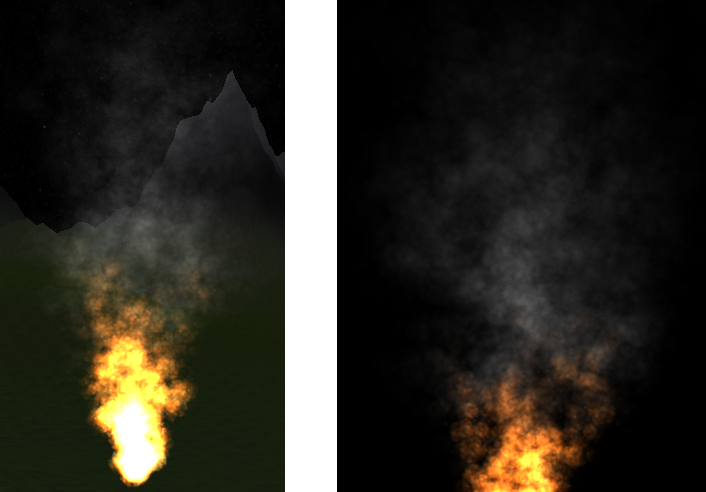
\includegraphics[width=\textwidth]{kepek/particleFireSmoke.png}
 \caption{Bal oldalon a tűz $\texttt{m\_fFireTimeRatio} = 0.25$ paraméterrel, jobb oldalon pedig a füst eloszlása közelebbről}
 \label{fig:particleFireSmoke}
\end{figure}

\subsubsection{Egyéb metódusok}
A részecskék rendezésére a későbbiekben az \texttt{std::sort} függvény segítségével kerül sor. Ennek azonban szüksége van az összehasonlításhoz valamilyen összehasonlító függvényre, vagy a $<$ operátor felüldefiniálására. Én az utóbbi megoldást választottam: 
\begin{cpp}
inline bool FireParticle::operator<(const FireParticle & rhs)
{
	return m_fDistanceToCamera > rhs.getDistanceToCamera();
}
\end{cpp}
Az \texttt{std::sort} ezt az operátort felhasználva növekvő sorrendbe teszi az objektumokat egy adott tárolón belül. Mivel a kamerától távolabbi részecskéket szeretném előbb kirajzolni, két részecske közül a nagyobb távolsággal rendelkezőt definiáltam kisebbnek.

A \texttt{FireParticle} osztály rendelkezik még jó néhány ``getter'' metódussal, melyek az árnyalóknak küldendő információkat adják vissza egyesével.

% Instancing & buffer re-specification
\subsection{Instancing és buffer re-specification}
Részecske rendszerek kirajzolásánál ugyanazt a ponthalmazt kell számtalanszor kirajzolni, csak más-más tulajdonságokkal. Az egyik lehetőség, hogy minden egyes részecskére meghívjuk a \texttt{glDrawArrays} metódust egy ciklusban. Ez egy működő megoldás, de ekkor minden hívás alkalmával a GPU teljes erejével azon lesz, hogy azt a 6 darab pontot megjelenítse, mely a billboard-hoz szükséges. Ennek kiküszöbölésére több megoldás is létezik, én az \textit{instancing} névre hallgató módszert választottam. 

Ennek lényege, hogy egyetlen alap ponthalmaz van (esetemben négyzet 6 pontból), de abból rengeteg példányt rajzol ki a grafikus gyorsítókártya egyszerre. Ehhez szükség van az alap pontokat tartalmazó pufferre, e mellé pedig csatolhatunk több puffert is, melyek az egyes példányok sajátos tulajdonságait írják le. Az OpenGL-nek minden egyes pufferről meg kell mondani, hogy 1 példányhoz hány elemet használjon fel belőle. Ezt a \texttt{glVertexAttribDivisor} metódus segítségével tehetjük meg. A kirajzolás pedig csupán annyiban különbözik a normálistól, hogy a \texttt{glDrawArraysInstanced} metódust kell használni, és megadni, hogy hány példányt kell majd létrehozni.

A példányok tulajdonságainak fenntartott VBO-kat tehát minden kirajzolás előtt frissíteni kell, azaz folyamatosan stream-eljük az adatokat a videokártyának. Ez azt jelenti, hogy feltöltjük a puffert adatokkal, majd a kirajzoláskor a GPU kiolvassa ezeket, de közben mi már ismét küldhetünk adatokat arra a pufferre, ami éppen olvasás alatt áll. Ahhoz, hogy ez ne okozzon hibát, az OpenGL specifikáció az \textit{implicit szinkronizáció} segítségével garantálja, hogy amíg a puffert olvassák, addig ne kerülhessen rá új adat, addig ugyanis az író szál fel van függesztve. Ez lassulást eredményezhet a program futása során. Ennek elkerülésére is számos módszer létezik, én a \textit{buffer re-specification}-t választottam, melyet az OpenGL dokumentációjában\footnote{https://www.khronos.org/opengl/wiki/Buffer\_Object\_Streaming} találtam.

 Ez a megoldás újrafoglalja a VBO-nak fenntartott memória területet a módosítás előtt. Ahhoz, hogy ez hatékony legyen, a \texttt{glBufferData} metódusban a \texttt{GL\_STREAM\_DRAW} konstans segítségével kell a videokártyával tudatni, hogy az adott puffert sokszor tervezzük törölni, majd újra létrehozni. A reallokálást a úgy érhetjük el, hogy adott VBO-ra meghívjuk a \texttt{glBufferData} metódust a korábbiakkal egyező paraméterekkel és \texttt{NULL} pointert adunk át neki az adatokra mutató paraméter helyén. Az OpenGL dokumentáció szerint ez teljesítmény szempontjából valószínűleg sokkal előnyösebb megoldás, mint az implicit szinkronizálásra hagyatkozni.

% FireParticleSystem
\subsection{FireParticleSystem osztály}
A részecskék karbantartását végző emitter a \texttt{FireParticleSystem} osztályban került implementálásra. A kibocsátáson, elpusztításon és a részecskék helyzetének aktualizálásán kívül ez az osztály felel a részecskerendszer kirajzolásáért, valamint rendelkezik egy \texttt{toggleWind} metódussal, melynek segítségével be- illetve kikapcsolhatjuk a szél hatást keltő ``erőt''. A tűz kirajzolásához tehát elég ezt az osztályt példányosítani, majd a \texttt{draw} metódusát meghívni a rendereléskor.

% fontosabb adattagok
\subsubsection{Fontosabb adattagok, paraméterek}
A tűz megjelenését a következő paraméterként is értelmezhető adattagok segítségével lehet befolyásolni:
\begin{itemize}
\item Maximális részecskeszám (\texttt{m\_iMaxParticles}): megadja, hogy maximum hány részecske lehet egyszerre életben.
\item Részecske élettartam (\texttt{m\_iParticleLifetime}): a részecskék élettartama ms-ban megadva. Minden részecske ennyi időt tölt majd a képernyőn, de mivel a sebességük eltérő, ez nem lesz feltűnő.
\item Az emitter pozíciója (\texttt{m\_vPosition}): e térbeli pont környékéről indulnak majd a részecskék.
\item A részecske rendszer skálája (\texttt{m\_fScale}): a részecskék méretére és a kiindulási terület nagyságára is hatással van.
\item Random generátorok (\texttt{m\_rRandom(...)}): többféle értékhatárok között generálnak pszeudo-random számokat. A részecskék indításához és példányosításához használom őket, ezek adják a rendszer véletlenszerűségét. Mindegyik egyenletes eloszlású értékeket generál.
\end{itemize}

% konstruktor
\subsubsection{Konstruktor}
A konstruktornak paraméterként meg kell adni a kamera és a tűz árnyaló objektumokra mutató pointereket és az emitter pozícióját. Opcionálisan megadható a maximális részecskeszám, illetve a skála paraméter is. Ezeket a megfelelő adattagokba lementem, majd emellett több más változó is inicializálásra kerül. 

Az \texttt{m\_pParticleContainer} tárolja majd a \texttt{FireParticle} típusú részecskéket, tehát akkorának kell lennie, hogy az összes részecskét egyszerre képes legyen tárolni:
\begin{cpp}
m_pParticleContainer = new FireParticle[maxParticles];
\end{cpp}

Az egyes példányok sajátos tulajdonságainak számontartásáért a következő pufferek felelnek:
\begin{cpp}
m_pPositionsBuffer = new float[maxParticles * m_iPositionElementCount];
m_pRotationAndBlendBuffer = new float[
			maxParticles * m_iRotationAndBlendElements];
m_pTexturesBuffer = new int[maxParticles];
\end{cpp}
Az \texttt{m\_pPositionsBuffer} tárolja majd a részecskék középpontjait és az adott részecske skála paraméterét (nem összekeverendő az egész részecske rendszer skála paraméterével), azaz részecskénként 4 db \texttt{float} értéket kell majd tárolnia. Az \texttt{m\_pRotationAnd\-BlendBuffer} tárolja a részecskék elfordulásának szögét, illetve a részecske pillanatnyi textúrájához tartozó blend paramétert, melynek segítségével az összemosást vagy az elhalványítást végzem fázistól függően. Az \texttt{m\_pTexturesBuffer} pedig a példányok pillanatnyi textúrájának sorszámát juttatja majd el a shader-nek.

A részecske rendszer egyik legmeghatározóbb paramétere tapasztalataim szerint az \texttt{m\_fParticlesPerSecond} származtatott adat, mely megadja, hogy másodpercenként hány részecske születhet. A kiszámítása az alábbi képlet alapját történik:

\begingroup
\Large
\begin{center}
$ \texttt{m\_fParticlesPerSecond} = \frac{\texttt{m\_iMaxParticles} \cdot 1000}{\texttt{m\_iParticleLifetime}}$
\end{center}
\endgroup
Minden részecske egyforma hosszú ideig él. Az indulás után pontosan \texttt{m\_iParticle\-Lifetime} időnek kell eltelnie, mielőtt az első részecskék elkezdenek meghalni. Ez azt jelenti, hogy ennyi idő alatt pontosan annyi részecskét lehet indítani, amennyi a tárolóban elfér (\texttt{m\_iMaxParticles}). Ezt követően pedig már megközelítőleg olyan iramban haláloznak el a részecskék, amilyen iramban születnek, tehát a részecskeszám nagyjából a maximum közelében fog maradni. Az 1000-el való szorzásra azért van szükség, mert az \texttt{m\_iParticleLifetime} mértékegysége ms.

A random generáló objektumok inicializálása után a konstruktor utolsó lépése a \texttt{loadBaseVAO} metódus meghívása. Ez a metódus betölti a tűz animálásához szükséges textúrát, majd létrehozza a rendszer VAO-ját. Ebben tárolom azokat a VBO-kat a tulajdonságaikkal együtt, melyek segítségével a fentebb említett pufferekben tárolt adatokat juttatom el a shader-eknek. 

%VBO-k betöltése
Az alap mesh-t tartalmazó VBO létrehozása hasonlít a billboard alapú tűznél alkalmazott módszerhez. Ezek a részecskék azonban minden irányba forgatva lesznek, így a négyzet középpontjának egybe kell esni az origóval, hogy az a transzformációnál ne mozduljon el. Az oldalak hossza 1, tehát a négy pont koordinátái: $(-0.5, -0.5, 0)$, $(0.5, 0.5, 0)$, $(-0.5, 0.5, 0)$, $(0.5, -0.5, 0)$.

A példányok tulajdonságait tartalmazó VBO-knak eltérő a megvalósítása a korábban tárgyalt problémákból kifolyólag. A részecske pozíciók és méretek tárolására használt OpenGL puffer létrehozása például a következőképpen néz ki:
\begin{cpp}
glGenBuffers(1, &m_iPositionsVBO);
glBindBuffer(GL_ARRAY_BUFFER, m_iPositionsVBO);
glBufferData(GL_ARRAY_BUFFER, 
	m_iMaxParticles * m_iPositionElementCount * sizeof(float), 
	NULL, GL_STREAM_DRAW); // buffer re-specification
glEnableVertexAttribArray(m_pFireShader->attrib("positionAndSize"));
glVertexAttribPointer(m_pFireShader->attrib("positionAndSize"), 
	m_iPositionElementCount, GL_FLOAT, GL_FALSE, 0, NULL);
// instancing hint
glVertexAttribDivisor(m_pFireShader->attrib("positionAndSize"), 1);
\end{cpp}
Ahogy azt a buffer re-specification módszernél már említettem, a \texttt{glBufferData} metódust csak allokálásra használjuk, és \texttt{ GL\_STREAM\_DRAW} konstanssal hívjuk meg. Az instancing módszerhez szükséges \texttt{glVertexAttribDivisor} metódus segítségével pedig jelezzük az OpenGL-nek, hogy példányonként 1 elemre van szükség az adott pufferből. A többi VBO előkészítése is hasonló módon néz ki, de természetesen a foglalt területek mérete eltér.

Egy érdekes hibára bukkantam azonban, mikor a textúrák sorszámát stream-elő VBO-t hoztam létre. A sorszámokat integerként tárolom, ennek megfelelően pedig jeleztem a videokártya felé a \texttt{glVertexAttribPointer}-en keresztül, hogy a pufferben tárolt adatok \texttt{GL\_INT} típusúak. A shader-ekbe azonban teljesen más számok érkeztek, mint amiket küldtem. A \textit{stackoverflow.com} oldalon már más is találkozott ezzel a problémával.\footnote{https://stackoverflow.com/questions/6578026/cant-get-integer-vertex-attributes-working-in-glsl-1-5} Itt arról ír a felhasználó, hogy annak ellenére, hogy a \texttt{GL\_INT} konstanst megadta, a kapott érték átkonvertálódik \texttt{float} típusúvá, majd ezt az árnyaló integerként olvassa ki. A nem túl elegánsnak tűnő megoldás pedig az, hogy a \texttt{glVertexAttribPointer}-nek  \texttt{GL\_FLOAT} paramétert kell átadni, így az nem konvertálja át a kapott integer értéket, tehát a shader helyesen tudja majd \texttt{int}-ként olvasni.

Így tehát a \texttt{loadBaseVAO} metódus előkészítette a szükséges VAO-t és benne a VBO-kat, valamint tulajdonságaikat.

% update
\subsubsection{A részecskék aktualizálása}
A részecskék frame-enkénti frissítéséért az \texttt{update} metódus felel. Itt történik a részecskék teremtése és pusztítása, a tulajdonságaik puffereinek aktualizálása illetve a szél, mint külső erő kalkulálása.

Első lépésként lekérdezem a \texttt{m\_pCamera} objektumtól az utolsó kirajzolás óta eltelt időt (ms). Ezt hozzáadom az utolsó részecske születése óta eltelt időhöz, hogy kiderüljön, eltelt-e már elég idő ahhoz, hogy új részecskét indítson útnak az emitter. A születendő részecskék számát úgy kapom, hogy az eltelt másodpercek számát megszorzom a másodpercenként kibocsátandó részecskék számával, és letárolom a szám egész részét a \texttt{newParticlesCount} lokális változóba.

Ezt követően aktualizálom a szélerőt a \texttt{calculateWindForce(elapsedTime)} metódushívással. Ez csupán annyit tesz, hogy amennyiben a szél ereje nem maximális, vagy éppen lassuló fázisban van (\texttt{m\_bStoppingWind} = \texttt{true}), akkor az állapotának megfelelően csökkenti, vagy növeli azt. Amennyiben a szél sebessége (\texttt{m\_fWindSpeed}) kisebb, mint $0$, akkor kikapcsolja azt (\texttt{m\_bWindIsBlowing} = \texttt{false}).

Utána aktualizálom az élő részecskéket:
\begin{cpp}
for (int i = 0; i < m_iNumberOfParticles; i++)
{
	FireParticle &fp = m_pParticleContainer[i];
	if (m_bWindIsBlowing) {
		fp.applyForce(m_vWindDirection, m_fWindSpeed);
	}
	if (!fp.update(elapsedTime)) {
		// if the particle died
		killParticle(i);
		// swap happend, 
		//the element at this index should be updated again
		i--;
	}
}
\end{cpp}
Ha fúj a szél, akkor beállítom azt, mint külső erőt minden aktív részecske esetén. A \texttt{FireParticle} osztály \texttt{update} metódusa igazzal tér vissza, ha a részecske még életben van, és hamissal, ha már nem. Utóbbi esetben a \texttt{killParticle} metódus segítségével meg kell szabadulni a részecskétől. 

% particle container and management
A részecskéket tároló \texttt{FireParticle} típusú tömb pontosan annyi elemből áll, amennyi a megengedett maximális részecskeszám. Így nem kell új elemeket beszúrni, sem régieket törölni, tehát a fix méretű tömb hatékonyabb, mint egy dinamikus lista. A könnyebb kezelhetőség érdekében az élő részecskéket a tömb első részében tartom, a holtakat pedig a végén, így nem kell az összes elemen végigiterálni frissítéskor, csak pontosan annyin, amennyi részecske életben van (\texttt{m\_iNumberOfParticles}). Ha egy részecske meghal, akkor kicserélem az utolsó élő elemmel. Részecske kibocsátáskor az új részecske az élő részecskék utáni első (halott) elem helyét veszi át. 

\Aref{fig:particleArray}. ábrán láthatjuk, hogy a \texttt{killParticle} hatására a halott részecske az élők mögé kerül (\texttt{std::swap}) közvetlenül, az utolsó élő részecske viszont átveszi a helyét. Ezért kell az iterációs változót eggyel csökkenteni, különben az előre helyezett részecske nem lenne frissítve.
\begin{figure}[h]
 \centering
 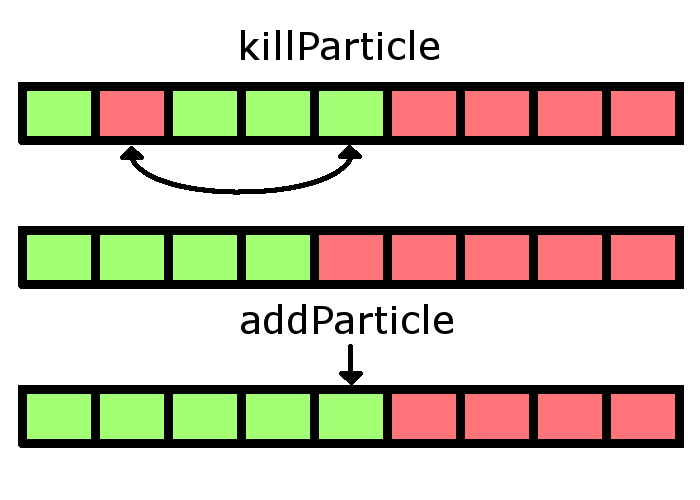
\includegraphics[width=0.6\textwidth]{kepek/particleArray.png}
 \caption{A részecske pusztulás és születés hatásai a tömbben.}
 \label{fig:particleArray}
\end{figure}

%addParticle
Ezt követően a \texttt{newParticlesCount}-nak megfelelő számú részecskét hozzáadok a tömbhöz az \texttt{addParticle} metódus segítségével, mely a következőképpen néz ki:
\begin{cpp}
if (m_iNumberOfParticles < m_iMaxParticles) {
glm::vec3 initialSpeed(m_rRandomXZ(m_rGenerator), 
	m_rRandomY(m_rGenerator), m_rRandomXZ(m_rGenerator));

float alpha = m_rRandomAngle(m_rGenerator);
float radius = m_rRandomRadius(m_rGenerator);
glm::vec3 offset = glm::vec3(m_fScale * cos(alpha) * radius, 
	0.f, m_fScale * sin(alpha) * radius);
		
m_pParticleContainer[m_iNumberOfParticles] = FireParticle(
	m_vPosition + offset, initialSpeed, alpha, m_iParticleLifetime, 
	m_pCamera, m_rRandomRotation(m_rGenerator));
m_pParticleContainer[m_iNumberOfParticles].update(0.f);
m_iNumberOfParticles++;
m_fTimeSinceLastEmittedParticle = 0.f;
}
\end{cpp}
Az \texttt{m\_rRandom} kezdetű adattagok csupán az értéktartományukban különböznek, a részecskék kiindulási paramétereinek véletlenszerűségével kapjuk a kellően kaotikus eredményeket. Az induló sebesség nem egységvektor, így a részecskék sebessége között még nagyobb különbségek keletkeznek. Az \texttt{offset} változó segítségével érem el, hogy a részecskék ne egy pontból induljanak ki, hanem az emitter pozíciójának adott sugarú körén belülről. Az \texttt{alpha} random változó a részecske kezdeti elfordulása is egyben. A \texttt{FireParticle} konstruktor utolsó paramétere a részecske elfordulásának szögsebessége. Az új részecskét az \texttt{m\_iNumberOfParticles} indexű elem helyére rakom, ez ugyanis az első elem a halott részecskék közül (\ref{fig:particleArray}. ábra). Az \texttt{update} metódus azonnali meghívására azért van szükség, hogy a részecske megfelelő adattagjai is értéket kapjanak, például a kamerától vett távolság és a textúra sorszám.

Az új részecskék tömbhöz adása után a kamerától vett távolság alapján sorba kell rendezni a tömb élő részecskéit. Ezt az \texttt{std::sort} függvény végzi el nekem a \texttt{FireParticle} osztály felüldefiniált $<$ operátora alapján. A függvénynek meg kell adni az adott tömb rendezni kívánt részének első és utolsó címét. Az utolsó címen található elem azonban nem kerül rendezésre, tehát valójában a még rendezni kívánt elem utáni címet kell megadni második paraméterként.

% VBO update
A rendezés után a példányok tulajdonságait feltölthetjük az ezeknek fenntartott pufferekbe:
\begin{cpp}
for (int i = 0; i < m_iNumberOfParticles; i++)
{
	FireParticle &fp = m_pParticleContainer[i];
	m_pPositionsBuffer[i*m_iPositionElementCount] = fp.getX();
	m_pPositionsBuffer[i*m_iPositionElementCount + 1] = fp.getY();
	m_pPositionsBuffer[i*m_iPositionElementCount + 2] = fp.getZ();
	m_pPositionsBuffer[i*m_iPositionElementCount + 3] = fp.getScale();

	m_pRotationAndBlendBuffer[i*m_iRotationAndBlendElements] = 
						fp.getRotation();
	m_pRotationAndBlendBuffer[i*m_iRotationAndBlendElements + 1] = 
						fp.getCurrentBlend();

	m_pTexturesBuffer[i] = fp.getCurrentTexture();
}
\end{cpp}
Az ezekhez tartozó VBO-kat pedig frissítjük az új adatokkal a buffer re-specification módszernek megfelelően. Ez a textúra sorszámokat tartalmazó VBO esetén a következőképpen néz ki:
\begin{cpp}
glBindBuffer(GL_ARRAY_BUFFER, m_iTexturesVBO);
glBufferData(GL_ARRAY_BUFFER, m_iMaxParticles * sizeof(int), 
			NULL, GL_STREAM_DRAW);
glBufferSubData(GL_ARRAY_BUFFER, 0, m_iMaxParticles * sizeof(int), 
			m_pTexturesBuffer);
\end{cpp}
A \texttt{glBufferData} hívással reallokáljuk számár a helyet, majd a \texttt{glBufferSubData} segítségével rámásoljuk az adatokat. Így a kirajzoláshoz szükséges vertex adatok már készen állnak.

% draw
\subsubsection{Kirajzolás}
A \texttt{draw} metódus hívásával történik meg a renderelés. Első lépésként az előbb tárgyalt \texttt{update} metódussal frissítem a részecskéket. 

% rotation with matrix tricks
Annak érdekében, hogy a billboard-ok mindig a kamera irányába forduljanak, az előző megoldástól eltérő módszert alkalmaztam. Ennek lényege, hogy a model és view mátrixok szorzatából (model-view) egy olyan transzformációs mátrixot kapjunk, melyben nincs forgatás. Ez azt jelenti, hogy a mátrix bal felső 3x3-as részmátrixa egységmátrix kell hogy legyen, amelyet úgy kaphatunk, hogy adott mátrixot a transzponáltjával szorzunk. A forgatások, melyeket ki szeretnénk küszöbölni a kamera mozgásából adódnak, és a view mátrixban találhatóak, tehát a model mátrix bal felső 3x3-as részmátrixa a view mátrix egyező részének a transzponáltjának kell lennie (\ref{fig:matrixRotation}. ábra). Így a billboard-ok forgatás nélkül lesznek kirajzolva, tehát mindig a kamera felé néznek (hiszen az alap négyzet az $XY$ síkon fekszik).
\begin{figure}[h]
 \centering
 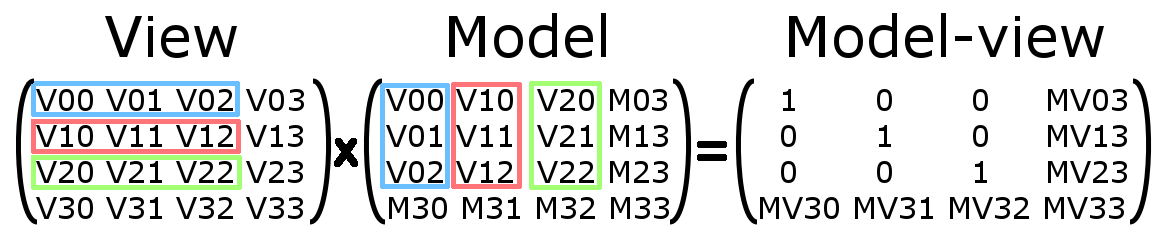
\includegraphics[width=\textwidth]{kepek/matrixRotation.png}
 \caption{A view és model mátrix szorzata a forgatás kioltásával}
 \label{fig:matrixRotation}
\end{figure}
Ezt a két mátrixot azonban nem szorzat formájában adom át a tűz árnyalónak, mert további transzformációk is szükségesek még, melyekkel még a view mátrix előtt kell megszorozni a model mátrixot (skálázás, $Z$ tengely menti forgatás, eltolás). A nézeti és projekciós mátrixot azonban átadhatom szorzatként, mellé pedig a modell mátrixot, a részecskerendszer skáláját, és a textúra sorainak számát is elküldöm a shader-nek (\texttt{fireShader.vs} és \texttt{fireShader.fs}) uniformként. Ezek után a lángok textúráját is átadom a \texttt{tex} uniform-ban. 

Ha a részecskerendszernek megadtuk a háttér mélység textúráját is, akkor azt, és az emitter kamerától vett távolságát is átküldöm a shader-nek. Ezekre a \textit{post-processing} során lesz szükség.

% additive(no sort, less particles) vs traditional blending, depth test
Mivel a textúra az alfa csatornájának teljes skáláját használja, szükség van valamilyen blending funkcióra is. Ezt még az OpenGL inicializációja során érdemes beállítani. Kezdésnek a billboard alapú tűz esetén használt tradicionális függvényt használtam, így \aref{fig:particleFireBasic1}. ábrán látható eredményt kaptam.

\begin{figure}[h]
 \centering
 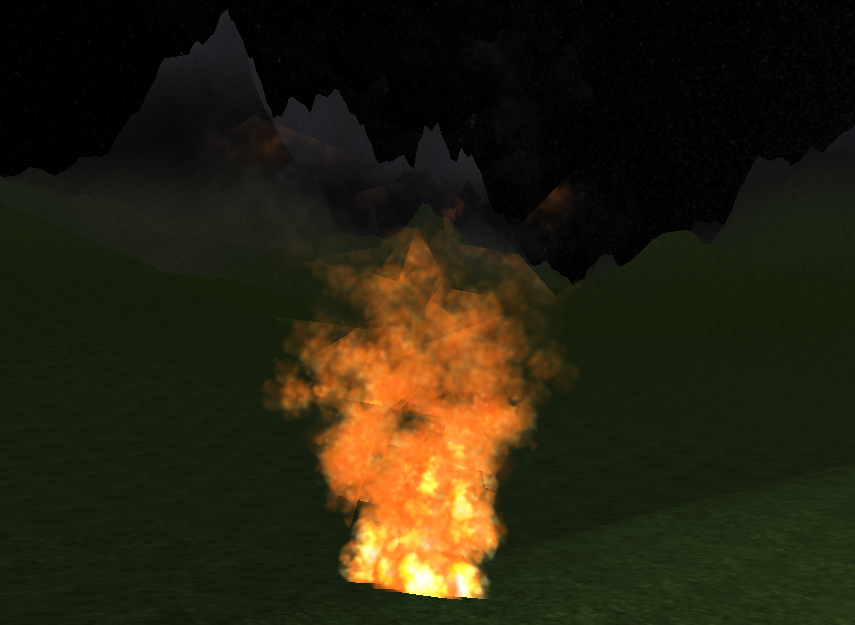
\includegraphics[width=\textwidth]{kepek/particleFireBasic1.png}
 \caption{Tradicionális blending és alapértelmezett mélységteszt (\texttt{GL\_LESS})}
 \label{fig:particleFireBasic1}
\end{figure}

Két probléma is felvetődik: 
\begin{itemize}
\item A rendezés ellenére is vannak átlátszósággal történő kitakarások.
\item A tűz túlságosan narancssárgának hat, és a kiindulásnál is furcsán robbanásszerű a részecskék kinézete.
\end{itemize}

Az első problémára nem találtam magyarázatot, lehetséges hogy a mélységben egymáshoz nagyon közel álló részecskék közt lép fel az anomália, bár ez csak nagyobb távolságokban jellemző. Az ilyen jelenséget egyébként \textit{z-fighting}-nak hívják, mely abból fakad, hogy a mélység puffer nem lineáris, így a közelebbi objektumok mélységét sokkal pontosabban méri, mint a távoliakét. De mivel esetemben közelről is jelentkezik a probléma, nem tartom valószínűnek, hogy ezzel állnék szemben. Megoldás azonban többféle is akad a problémámra.

% glDepthMask(False) vs glDepthFunc(GL_ALWAYS)
A mélység puffer a színpufferhez hasonlóan pixelenként tárolja az információt. A feladata, hogy a nézőponthoz közelebbi objektumokat ne takarják ki az attól távolabbiak. Ha engedélyezve van a használata, akkor a fragment shader kimeneti értékének a mélységét összeveti a pufferben az annak megfelelő helyen tárolt értékkel. Ha az új kimenet értéke nagyobb, azaz távolabb van a kamerától, akkor nem íródik be az érték sem a mélység, sem a szín pufferbe. 

A kitakarás tehát a mélységtesztből fakad, ezt azonban nem érdemes kikapcsolni. Helyette az jelentené a megoldást, hogy kirajzoláskor az adott fragment mindenképpen átmegy a teszten. Az egyik lehetőség, hogy a részecskék mélységértékeit nem írjuk be a pufferbe, így nincs ami kitakarjon. A másik megoldás a mélységteszt összehasonlító funkciójának a megváltoztatása.

Ha a kirajzolt objektum mélységét nem szeretnénk beírni a mélység pufferbe, akkor a \texttt{glDepthMask(GL\_FALSE)} hívás segítségével a mélység puffer írását kikapcsolhatjuk. A mélység teszt továbbra is működik, tehát a kitakart objektumok nem fognak látszódni. Azon objektumok azonban, melyek nincsenek takarásban kirajzolódnak, de a mélységük nem kerül be a pufferbe. Így tehát a föld felett lévő összes részecske színe bekerül a színpufferbe, illetve összemosódik az ott tárolt értékkel, tehát nem történik átlátszósággal való kitakarás. A kirajzolás után a mélységpuffer írását ekkor a \texttt{glDepthMask(GL\_TRUE)} hívással engedélyezhetjük megint.

\begin{figure}[h]
 \centering
 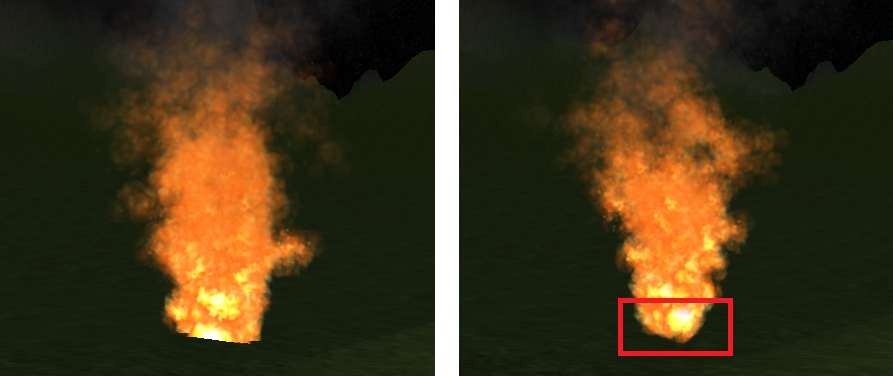
\includegraphics[width=\textwidth]{kepek/particleDepthComparison.png}
 \caption{Bal oldalon a mélység puffer írása volt kikapcsolva, jobb oldalon az összehasonlító funkció \texttt{GL\_ALWAYS}-re lett beállítva.}
 \label{fig:particleDepthComparison}
\end{figure}

A másik megoldás a mélységteszt módszerének átállítása. Ezt a \texttt{glDepthFunc} függvény segítségével lehet manipulálni, az alapértelmezett tesztmód a \texttt{GL\_LESS}. Mikor a kirajzolandó fragment mélységértéke összehasonlításra kerül a mélységpuffer megfelelő helyén tárolt értékkel, akkor a \texttt{GL\_LESS} szerint a kisebbik érték lesz az érvényes, tehát a kamerához közelebbi fragment mélysége felülírja pufferben tároltat. Számomra viszont a \texttt{glDepthFunc(GL\_ALWAYS)} hívás nyújtja az elérni kívánt hatást. Ez azt eredményezi, hogy mikor a két érték összevetődik, az aktuálisan kirajzolni kívánt fragment értéke mindenképpen felülírja a mélységpufferben tárolt értéket, azaz a fragment (színnel együtt) elfogadásra kerül. Így megközelítőleg helyes mélységértékek szerepelnek majd a tűz helyén a mélységpufferben, amennyiben erre szükségünk van (a post-processing során lesz is). 

Az utóbbi módszer hátránya viszont, hogy az így kirajzolt objektum minden mást kitakar, olyasmit is, ami előtte lenne. Ebben az esetben a tűz föld alatti része is ki fog látszani (\ref{fig:particleDepthComparison}. ábra piros négyzet), illetve ha néhány farönk tetején égne, akkor azokat is csúnyán kitakarná. Így ha csak egyszerűen kirenderelünk mindent a képernyőre, és nincs szükségünk a kirajzolt objektum mélység értékeire, a mélység puffer kikapcsolása jelenti a jobb megoldást.


% additive blending
A második probléma (a tűz színe) okát a blending függvényben kell keresni. A tűz és hasonló jelenségek részecske rendszerrel történő megjelenítése során gyakran alkalmazzák az ún. additív blending-et, és az általam használt textúrát is valószínűleg erre tervezték. Én az alábbi színkeverési funkciót alkalmaztam: 
\begin{cpp}
glBlendFuncSeparate(GL_SRC_ALPHA, GL_ONE, GL_SRC_ALPHA, GL_ONE);
\end{cpp}
Mint azt már láthattuk, az első két paraméter a színek keverését befolyásolja, a második kettő pedig az alfa csatornákra vonatkozik. Akár csak a tradicionális blending esetén, a két művelet itt is összeadás. 
\begin{figure}[h]
 \centering
 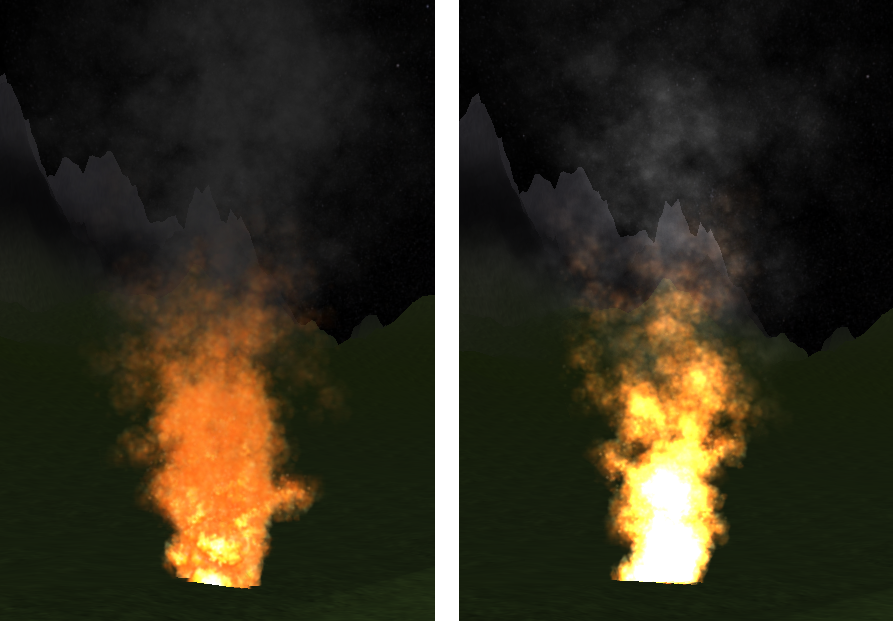
\includegraphics[width=\textwidth]{kepek/particleBlendingComparison.png}
 \caption{Bal oldalon a tradicionális összemosás, jobb oldalon az additív.}
 \label{fig:particleBlendingComparison}
\end{figure}

A fragment színe a saját alfa értékének arányában van elhalványítva, ezt adjuk hozzá a háttér változatlan színéhez. Ebből következik tehát, hogy a tradicionális blending-nél egy sokkal világosabb eredményt kapunk. Ha egy fragmenten több ilyen művelet is elvégződik, akkor az eredmény egyre fehérebb lesz, végül teljesen fehérré válhat. Ez különösen is hasznos a tűz esetén, ahol ha több részecske is van egymáshoz közel, akkor ott nagyobb is a jelenség ``hőmérséklete'', és -- ahogy annak lenni kell -- így fehérebb is lesz a színe (\ref{fig:particleBlendingComparison}.ábra jobb oldala). Mivel úgyis minden részecske színe hozzáadódik a színpufferhez, a részecskék kirajzolásának sorrendje a kinézeten nem változtat, tehát a sorbarendezést akár ki is hagyhatnánk. A post-processing során azonban a mélység értékekre is szükség lesz, tehát a rendezés a mélység puffer helyességét hivatott biztosítani ebben az esetben.

A kinézeten nem változtat, hogy az alfa csatornákat hogyan keverjük egymással, azonban a post-processing során részben pont az alfa értékek határozzák meg a torzítás mértékét, így az aktuális fragment alfa csatornáját ugyanúgy additívan keverem a háttér alfájával.

A mélységpuffer írásának kikapcsolása és a színkeverés engedélyezése után kirajzolhatjuk végre a részecske rendszert.
\begin{cpp}
glBindVertexArray(m_iParticleVAO);
glDrawArraysInstanced(GL_TRIANGLES, 0, 6, m_iNumberOfParticles);
\end{cpp}
Az instancing módszernek megfelelően a hívás utolsó paramétereként meg kell adni, hogy hány példányt rajzoljon ki az OpenGL. Ezt követően vissza lehet kapcsolni a mélységpufferek írását, illetve ki kell kapcsolni a blending-et is.

% fire shader
\subsection{Tűz árnyaló}
A billboard alapú megjelenítéssel ellentétben az instanced renderelés miatt a shader-eknek itt már lényegesen több feladat jut. 

\subsubsection{Vertex shader}
A vertex árnyaló lesz felelős a példányok tulajdonságaiként megkapott eltolás, forgatás és skálázás elvégzéséért az adott ponton, valamint a hozzá tartozó textúra koordináták kiszámításáért. Uniform-ként megkapja a transzformációs mátrixokat (view-projection és model), a részecskerendszer skáláját, valamint a textúrán lévő állapotok sorainak számát (\texttt{rowCount}). Csúcspontonként pedig megkapja az adott példány textúrájának sorszámát(\texttt{textureNr}), a pozícióját, a skáláját, az elfordulásának szögét és az összemosáshoz szükséges blend paramétert. 

Elsőként a blend paramétert át is passzolom a fragment árnyalónak (\texttt{currentBlend}), mert csak ott lesz rá szükség. Ezt követően a textúra koordinátákat határozom meg. Hasonlóan történik billboard alapú tűznél alkalmazott módszerhez, de itt nem számoljuk ki a négyzet mind a 4 pontjához szükséges koordinátákat, csupán azt kapjuk meg, amelyik pontot éppen feldolgozza az árnyaló. Ezt a \texttt{vec2 getTextureCoord(int textureNr, float offset)} függvény számolja ki \aref{fig:particleBillboard}. ábrán látható értékeknek megfelelően.

\begin{figure}[h]
 \centering
 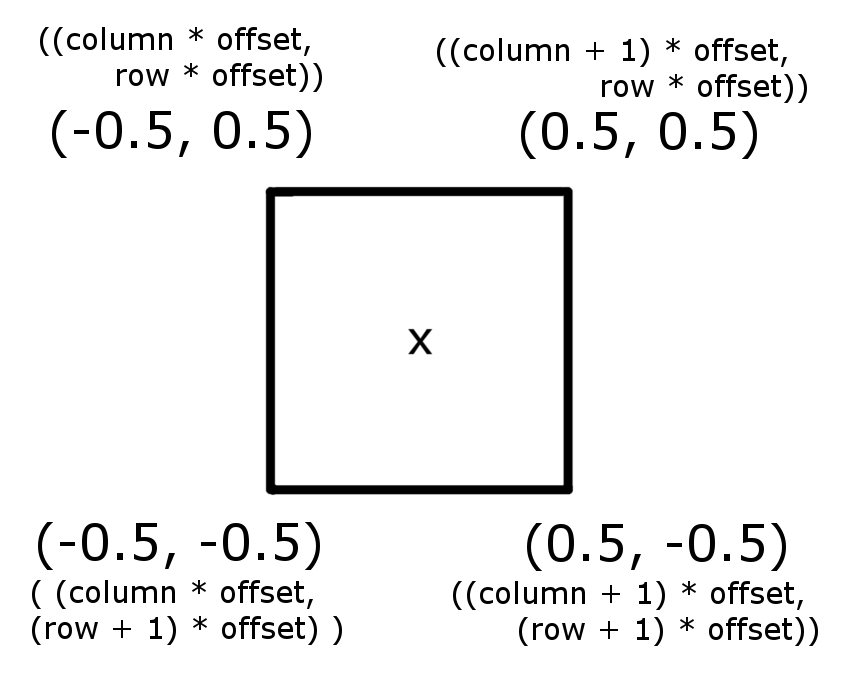
\includegraphics[width=0.7\textwidth]{kepek/particleBillboard.png}
 \caption{A számok az $x$ és $y$ koordináták, a szöveges részek pedig a megfelelő állapot textúra koordinátái.}
 \label{fig:particleBillboard}
\end{figure}

Az \texttt{offset} változó egy állapot szélességét adja meg a textúra koordinátáknak megfelelően $(\frac{1}{\texttt{rowCount}})$. Azt, hogy a négyzetnek éppen melyik sarkát dolgozza fel az árnyaló, \texttt{if} szerkezetekben lévő feltételek segítségével határolom be. A \texttt{textureNr} segítségével a billboard alapú tűznél alkalmazott képlet segítségével kiszámolom, hogy hányadik sor (\texttt{row}) hányadik oszlopában (\texttt{column}) található a keresett rész, majd \aref{fig:particleBillboard}. ábrán látható számolások után visszatérek a megfelelő textúra koordinátákkal.

Ha a pillanatnyi textúra sorszáma nem a legutolsó textúrára mutat, akkor a következő állapot ezen ponthoz tartozó textúra koordinátáit is kiszámolom a \texttt{getTextureCoord} függvénnyel. Ezeket át is adom a fragment shader-nek a \texttt{fragTexCoord} és a \texttt{fragTexCoord2} változók segítségével. Ekkor a \texttt{smoke} változó 0, ez mutatja meg ugyanis, hogy a füst fázisban van-e az adott példány. Ezt a változót a \texttt{flat} módosító segítségével tudom átadni a fragment shadernek, ugyanis ez nem interpolálható. Ezzel szemben ha a pillanatnyi textúra állapot az utolsó, akkor a rákövetkezőt természetesen már nem számoltatom ki, és a \texttt{smoke} változó is megkapja az 1-es értéket.

Most már csak a kapott csúcspont transzformációit kell elvégezni. A példány tulajdonságaiként kapott adatok segítségével előállítom a skála (\texttt{scalingMatrix}), a forgatás (\texttt{rotationMatrix}) és az eltolás (\texttt{translationMatrix}) mátrixokat, majd ezeket a megfelelő sorrendben összeszorzom:
\begin{cpp}
mat4 particleMatrix = translationMatrix * model * rotationMatrix
							 * scalingMatrix;
\end{cpp}
Mint azt már korábban is tárgyaltuk, a \texttt{model }mátrix a kamera mozgásából fakadó forgatásokat küszöböli ki, tehát az is forgatás transzformációkat végez, így még az eltolás előtt kell vele is szorozni.

A transzformált csúcspontot végül a következőképpen kapjuk:
\begin{cpp}
gl_Position = viewProjection * particleMatrix * vec4(vert, 1);
\end{cpp}


\subsubsection{Fragment shader}
A fragment shader feladata, hogy a bemenetként kapott, interpolált adatok segítségével mintavételezze a textúrát, és előállítsa a fragment színét. Ha a \texttt{smoke} változó nem 1, akkor a pillanatnyi és a következő állapot textúra színeit keveri össze a \texttt{currentBlend} változó segítségével:
\begin{cpp}
finalColor = vec4(currentBlend * textureColor.rgba 
	     + (1 - currentBlend) * textureColor2.rgba);
\end{cpp}

Viszont ha a láng füst fázisban van, akkor az általam megadott szürke szín kerül az RGB komponensekbe, az A komponenst pedig a textúra alfa csatornája és a \texttt{currentBlend} szorzata adja: 
\begin{cpp}
finalColor = vec4(vec3(0.2f,0.2f,0.2f), currentBlend * textureColor.a);
\end{cpp}

Ezekkel eddig majdnem tökéletes az eredmény, de a narancs színű lángból való átmenet a szürke színű füstbe így hirtelen történik. Ennek csillapítását a következőképpen oldottam meg:
\begin{cpp}
float blendWithOldColor = currentBlend - 0.85f;
if(blendWithOldColor > 0.f) {
   blendWithOldColor = blendWithOldColor / 0.15f;
   finalColor = vec4((1.f - blendWithOldColor) * vec3(0.2f,0.2f,0.2f) 
   + blendWithOldColor * textureColor.rgb, currentBlend * textureColor.a);
}
\end{cpp}
Ekkor a \texttt{currentBlend} tulajdonképpen a részecske kora a füstfázisban, mely $1$-ről indul és $0$-ig csökken folyamatosan. Így ebből az $1$ hosszúságú tartományból $0.15$ hosszúságnyit az összemosásra szántam. A \texttt{blendWithOldColor} változóban tartom számon, hogy mennyi van még hátra az átmeneti időszakból és annak arányában mosom össze a szürke színt a textúra színével egyszerű lineáris interpolációval.

Ezek segítségével, és szél (mint külső erő) hozzáadásával \aref{fig:particleWind}. ábrán látható eredményt kapom.
\begin{figure}[h]
 \centering
 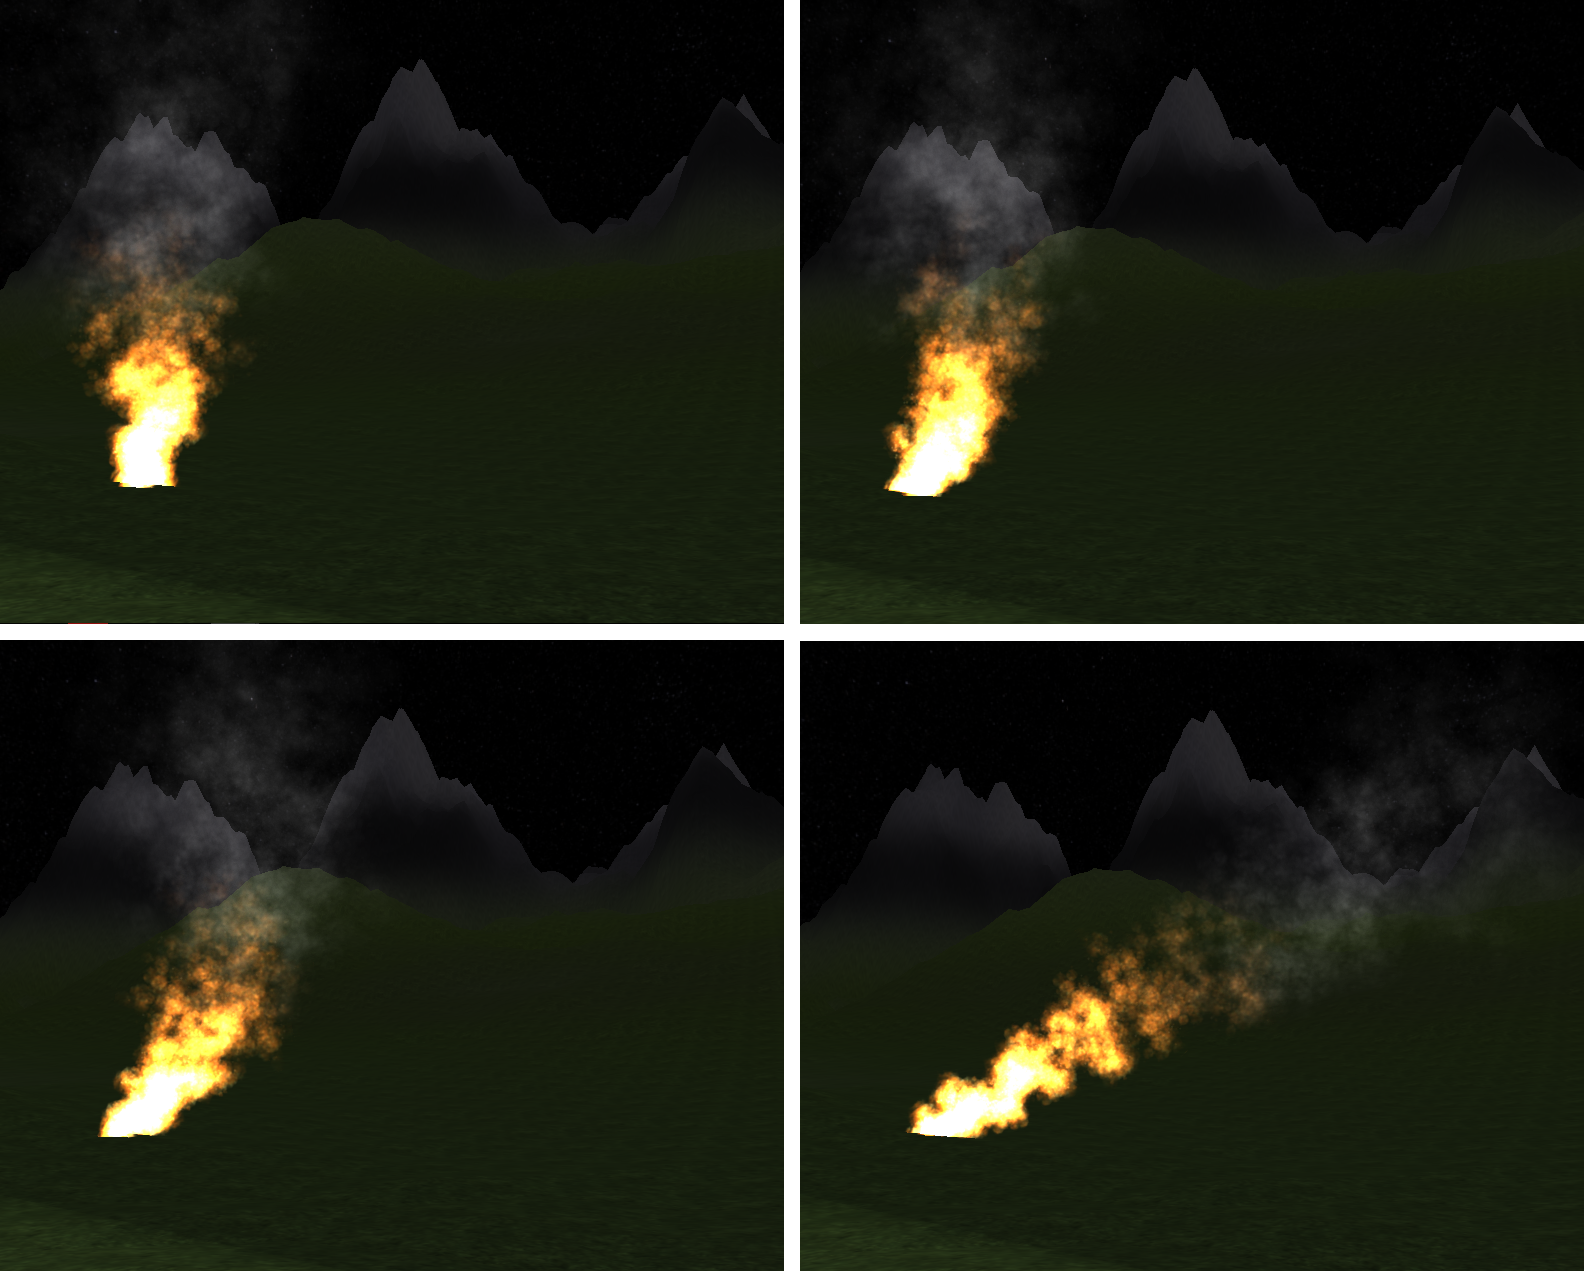
\includegraphics[width=\textwidth]{kepek/particleWind.png}
 \caption{A szél ereje fokozatosan nő, kikapcsolásnál pedig fokozatosan csökken.}
 \label{fig:particleWind}
\end{figure}

%%%%%%%%%%%%%%%% Post processing
\subsection{Post-processing}
A hő hatásából fakadó fénytörés megjelenítéséhez egy újabb trükköt kell alkalmazni. A post-processing az a folyamat, melynek során a kirajzolt eredményt, mint képet módosítjuk. A jelenetet tehát nem a képernyőre, hanem egy textúrára kell renderelni, majd a textúrát egy billboardon kell megjeleníteni, mely az egész képernyőt befedi. Azonban ha mindent egyszerre egy képre rajzolunk ki, akkor távolságtól és takarástól függetlenül mindent csak egyszerre torzíthatunk. Így érdemesebb a jelenet külön részeit külön képekre kirajzolni, a megfelelőeket módosítani, majd összerakni a végeredményt elemenként.

A fénytörés megvalósítását úgy képzeltem el, hogy a hátteret és a tüzet külön képekre renderelem ki, majd a háttér megfelelő részét módosítom, végül a torzított eredményre rárajzolom a tüzet is, így azt nem éri torzítás.

% FBO
\subsubsection{Frame buffer object}
A textúrára való renderelést \textit{frame buffer object}-ek\footnote{https://www.khronos.org/opengl/wiki/Framebuffer\_Object} (FBO) segítségével végezhetjük el. Az FBO-k framebuffer-eket fognak egységbe, és lehetővé teszik az ezekre történő kirajzolást. Ilyenek lehetnek például a szín, mélység és stencil pufferek. Szín pufferből többet is tartalmazhat, mélység pufferből viszont csak egyet, de azt kötelezően, ha renderelni is szeretnénk rá. 

A felhasználástól függően ezek a pufferek is különböző típusúak lehetnek. Ha csak renderelni szeretnénk rájuk, mintavételezni nem akarjuk őket, akkor az erre optimalizált \textit{renderbuffer} objektum a helyes választás. Azonban nekem szükségem lesz mind a mélység, mind a szín értékekre más helyeken is, tehát nekem mindkét pufferem textúra lesz. Így lehet őket árnyalóknak is átadni, és ott olvasni belőlük. 

% PostProcessor class
\subsubsection{PostProcessor osztály}
A fénytörés megvalósítására készítettem egy osztályt, mely FBO-ként funkcionál. Több példányra is szükség lesz belőle, mindegyik más és más funkciót lát majd el.

Az osztály konstruktorának meg kell adni a képernyő magasságát és szélességét, valamint a kirajzoláshoz használandó shader fájlok nevét. Betölti az árnyalókat, majd meghívja az \texttt{initializeFBO} és \texttt{generateVAO} metódusokat.

% render textures
Az \texttt{initializeFBO} metódus legenerál egy, a képernyő méretnek megfelelő magasságú és szélességű kétdimenziós textúrát, mely a színpuffer szerepét veszi majd fel. Ez \texttt{RGBA} formátumú lesz, egyes elemei pedig \texttt{unsigned byte} típusúak. A mélység puffer számára is egy ugyanolyan méretű, de eltérő paraméterezésű kétdimenziós textúrát hoztam létre. Ennek formátuma \texttt{GL\_DEPTH\_COMPONENT} lesz. Ezen kívül további, a mélységpuffert jellemző paramétereket is be kellett állítani:
\begin{cpp}
glTexParameteri(GL_TEXTURE_2D, GL_DEPTH_TEXTURE_MODE, GL_INTENSITY);
glTexParameteri(GL_TEXTURE_2D, GL_TEXTURE_COMPARE_MODE, 
						GL_COMPARE_R_TO_TEXTURE);
glTexParameteri(GL_TEXTURE_2D, GL_TEXTURE_COMPARE_FUNC, GL_LEQUAL);
\end{cpp}
Az első sor megadja, hogy a mélység értékeket hogyan kezelje az OpenGL mintavételezés során. A második hívás mondja ki, hogy az újonnan bekerülő értékeket össze kell hasonlítani a már jelenlevő értékekkel, az ezt követő hívás pedig az összehasonlítás módját adja meg.

Utolsó lépésként a metódus legenerálja az FBO-t is, majd az imént létrehozott textúrákat csatolja hozzá, mint szín és mélység puffereket.

A \texttt{generateVAO} metódus legenerálja a megjelenítéshez szükséges négyzetet. Az OpneGL-ben nézeti transzformációk nélkül a kamera a $(0, 0, 0)$ pozícióban van, és a $-Z$ tengely felé néz. Az OpenGL specifikáció szerint az alapértelmezett nézet egy 2x2-es méretű kockát lát. Ebből következik, hogy a képernyő négy sarkában a $(-1, -1)$, $(1, 1)$, $(-1, 1)$, $(1, -1)$ pontok láthatóak. Tehát ha olyan négyzetet szeretnénk kirajzolni amely transzformációk nélkül pont beteríti a képernyőt, akkor annak pont ezek lesznek a csúcspontjai.

\subsubsection{Kirajzolás}
Az osztályhoz hozzáadhatunk:
\begin{itemize}
\item Egy további textúrát, mint színes képet (\texttt{addTexture(GLuint textureId)}). Ez az árnyaló \texttt{tex2} uniform-jába kerül.
\item Egy előtérhez és egy háttérhez tartozó mélység textúrát (\texttt{addBackgroundDepth\\(GLuint textureId)}, \texttt{addForegroundDepth(GLuint textureId)}).  Ezek az árnyaló \texttt{foreground\-Depth} és \texttt{backgroundDepth} uniform-jaiba kerülnek.
\item Végül pedig egy \texttt{float} típusú offszetet (\texttt{setOffset(float offset)}), mely a shader \texttt{offset} uniform-jába kerül.
\end{itemize}
Az ezek tárolására szolgáló adattagokat \texttt{NULL} értékkel inicializáltam, így a kirajzolást végző \texttt{draw} metódus csak akkor adja át ezeket az árnyalóknak uniform-ként, ha az értékük ettől eltérő. 

A \texttt{draw} metódus opcionális paramétere (\texttt{bool renderOwnTexture}) azt adja meg, hogy a kirajzolásnál textúraképpen a saját színpufferét is csatolja-e, ugyanis szükség lesz majd arra is, hogy egy hozzáadott textúrát felhasználva a saját színpufferébe rajzolja ki a jelenetet.

A metódus tehát a feltételes uniform beállítások után kirajzolja a VAO-jában tárolt $4$ pontot \texttt{GL\_TRIANGLE\_STRIP}-ként.

A későbbiekben a \texttt{PostProcessor} osztályhoz rendelt vertex shader-ek mind ugyanolyanok. Bemenetként megkapják a csúcspontokat, melyeken nem is végeznek transzformációt, csupán kibővítik egy homogén koordinátával. Kimenetként produkálnak még egy \texttt{fragTexCoord} textúra koordinátát. Itt egyszerű dolga van az árnylónak, a pontok koordinátáinak az értéktartományát kell leszűkíteni $[-1, 1]$-ről $[0, 1]$-re. Hozzáad a vertex elemeihez 1-et, majd elosztja őket 2-vel, és meg is vannak a megfelelő textúra koordináták. A fragment shader-ek ellenben már bonyolultabbak lesznek, ezek végzik gyakorlatilag a képek módosítását. Minden művelethez más és más árnyalóra lesz majd szükség.

%postprocessing steps and shaders
\subsubsection{Fénytörés az FBO-k segítségével}
A fénytörés megvalósítását több lépésben képzeltem el. Egy textúrára ki kell rajzolni a hátteret (ég, domborzat), hogy azt később torzítani lehessen. Egy másik textúrára a tüzet rajzolom ki, hogy azt majd torzítás nélkül a torzított háttérre rajzolhassam. Ahhoz, hogy a háttér megfelelő (tűz mögötti) részét be tudjam határolni a torzításhoz, szükség van valamilyen maszkra. Erre a célra a kirajzolt tűz képét fogom módosítani, és azt, mint maszkot felhasználva torzítom majd el a hátteret. 

A \texttt{PostProcessor} osztályt általában úgy használom fel, hogy kirajzolok a pufferébe egy jelenetet, majd ezt textúraként felhasználva az árnyalója segítségével valamilyen post-processing műveletet elvégezve kirajzolom a feldolgozott képet. Utóbbit a képernyőre, vagy egy másik FBO-ba is irányíthatom. Az effekt megvalósításához négy különböző \texttt{PostProcessor} objektumra van szükségem:
\begin{itemize}
\item  \texttt{renderedBackground}: Ebbe az objektumba rajzolom ki torzítás mentesen a hátteret, majd a \texttt{draw} metódusa segítségével a hozzáadott maszk textúra alapján képes torzítva kirenderelni azt. Ez az objektum a \texttt{postprocessor} árnyalót használja majd kirajzolás során.
\item \texttt{renderedFire}: Ebbe az objektumba rajzolom a részecske rendszer alapú tüzet. A \texttt{noEffectFBO} shader segítségével ezt változatlanul rajzolja ki a \texttt{draw} metódusával.
\item \texttt{distortionMap}: Ennek az objektumnak eltér a felhasználása a többitől. Először hozzá csatolom textúraként a kirenderelt tüzet, ebből pedig a \texttt{createDistortion\-Map} árnyaló segítségével kirajzolja a maszkot a saját FBO-jába. Ezt aztán később csatolni lehet textúraként a \texttt{renderedBackground}-hoz.
\item \texttt{finalPicture}: Ebbe az objektumba rajzolom ki a torzított hátteret, majd csatolom hozzá a kirajzolt tüzet, illetve az előtér (tűz) és háttér (domborzat) mélység puffereit textúraként. A \texttt{blendPictures} shader pedig a mélységteszt elvégzésének segítségével összevágva kirajzolja a végső jelenetet.
\end{itemize}
A lépéseket nagy vonalakban \aref{fig:postprocessing}. ábrán láthatjuk.
\begin{figure}[h!]
 \centering
 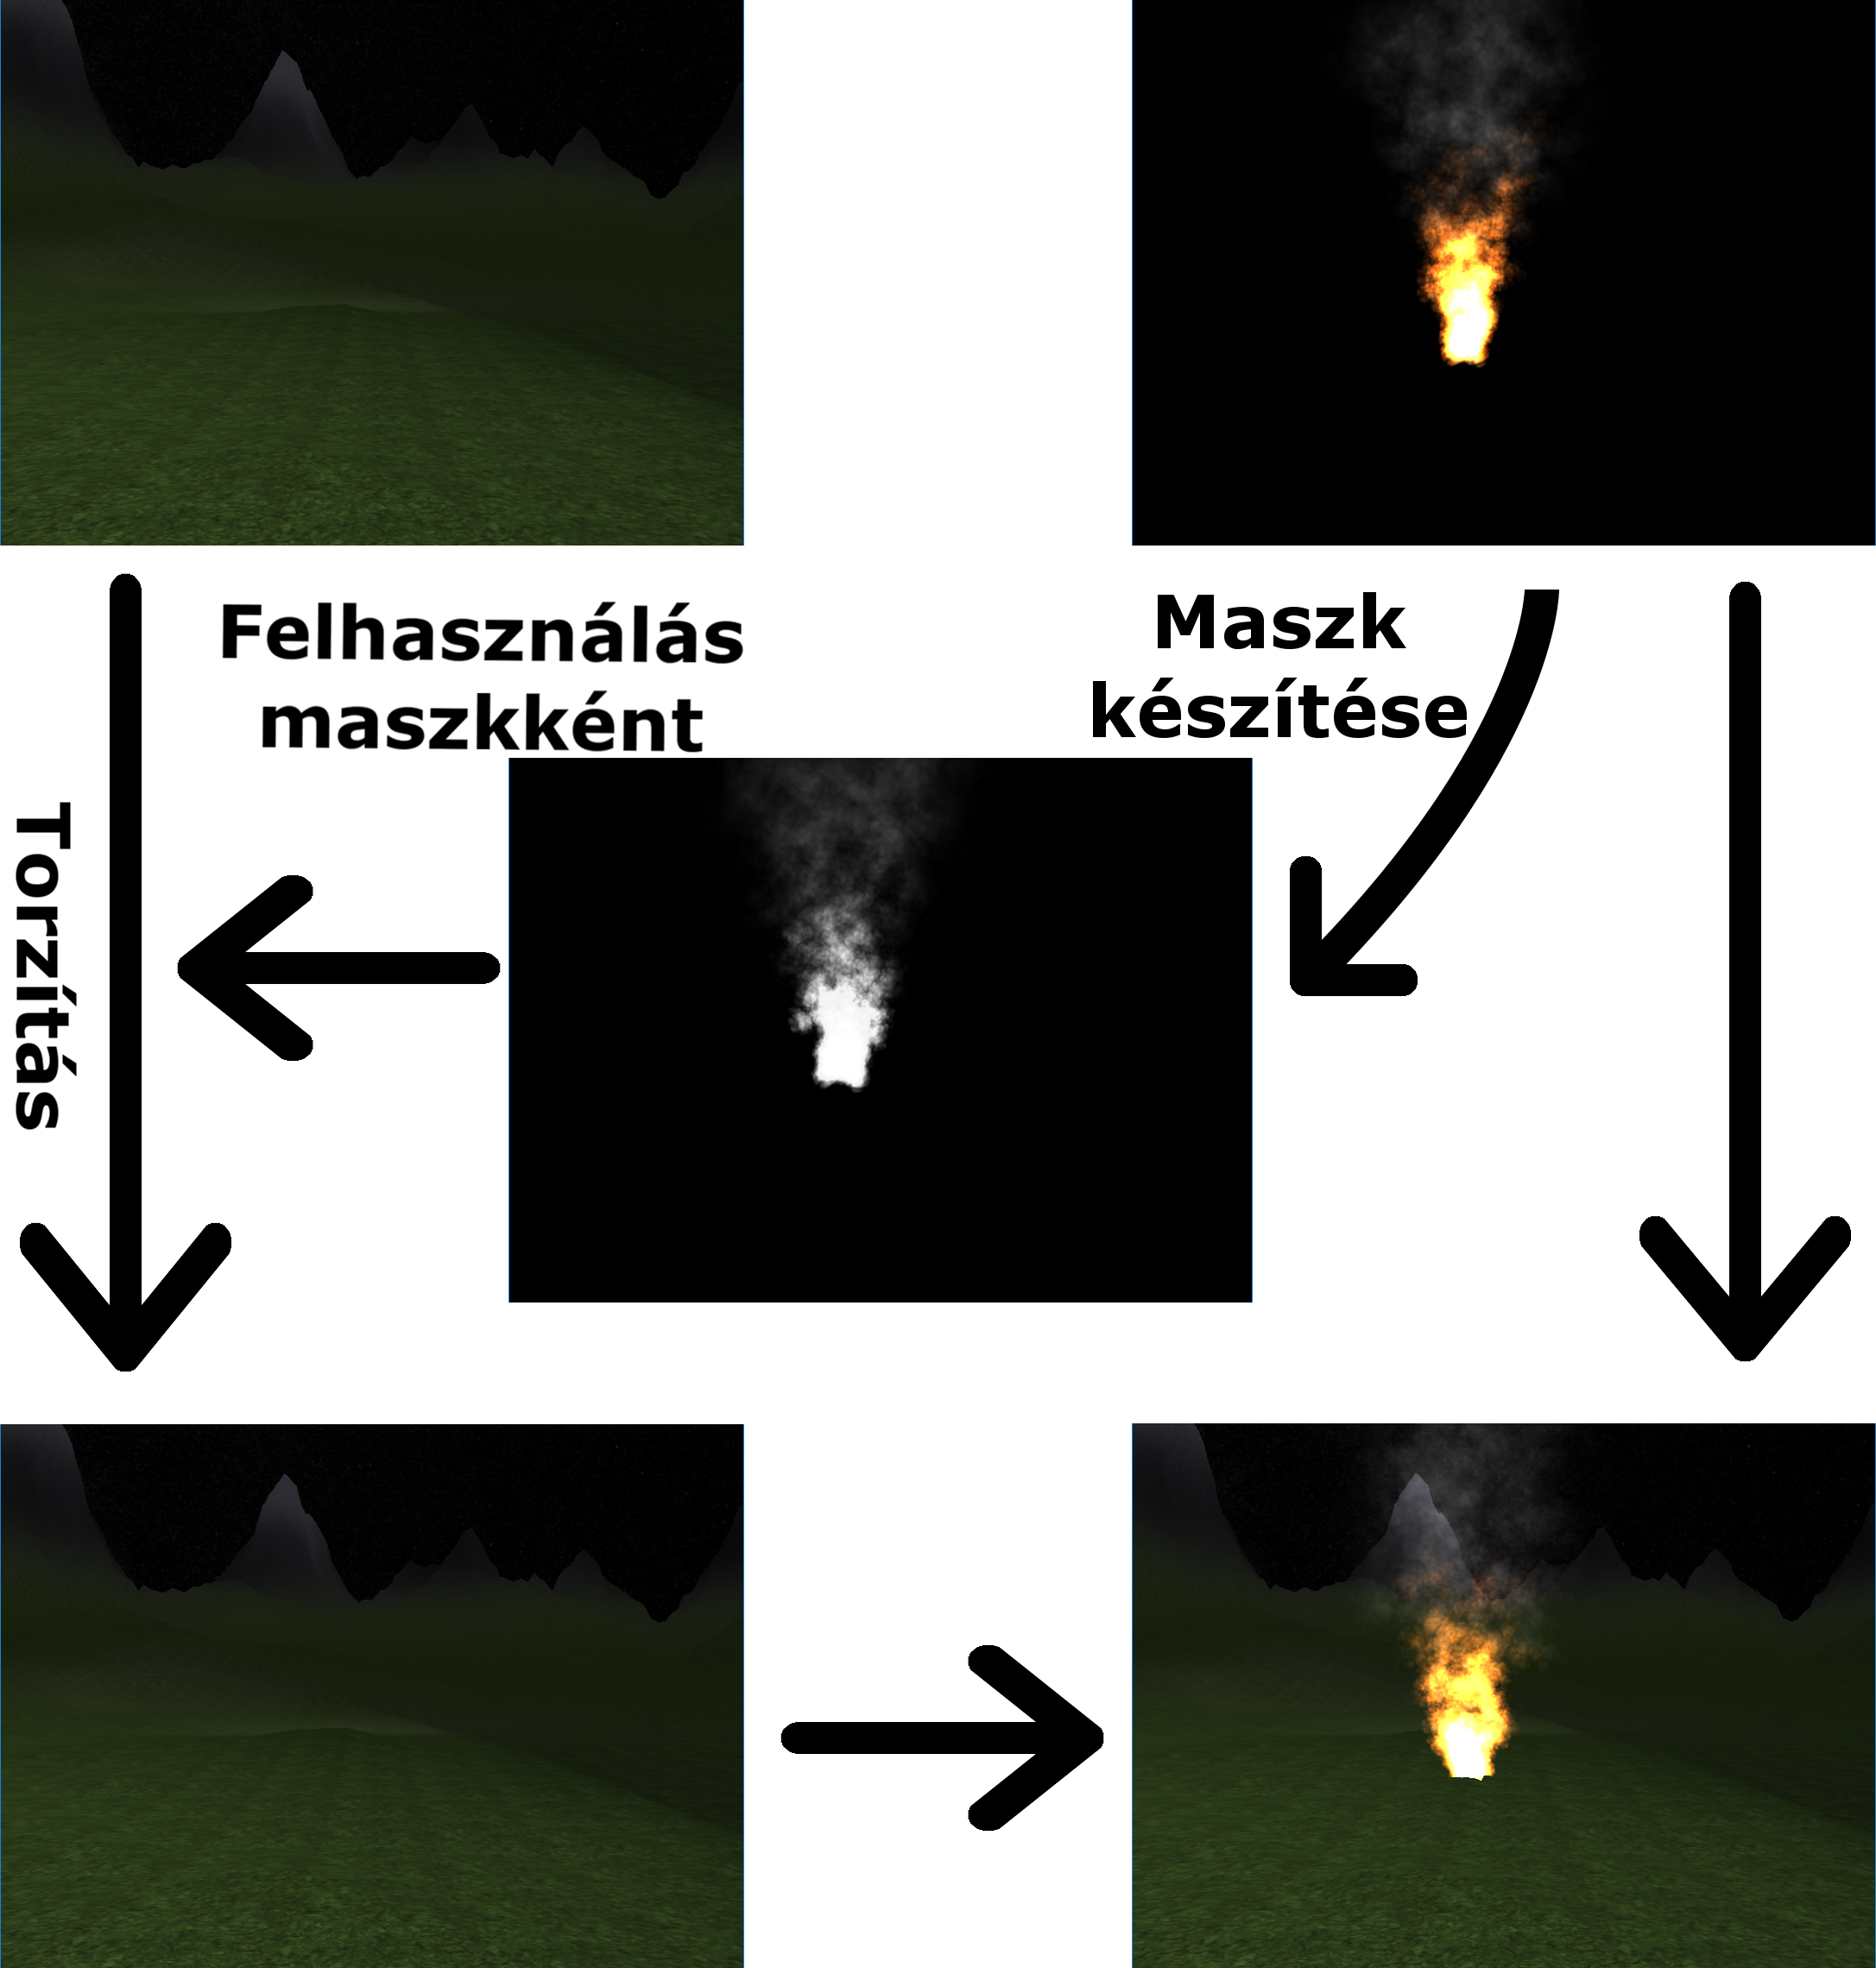
\includegraphics[width=\textwidth]{kepek/postprocessing.png}
 \caption{A torzítást a hegy oldalán lehet észrevenni.}
 \label{fig:postprocessing}
\end{figure}
A post-processing logikát a \texttt{main.cpp} fájlban a \texttt{display} függvényben implementáltam.

Először tehát a \texttt{renderedBackground} objektumba kirajzolom a hátteret, majd a \texttt{renderedFire}-be a tüzet (\ref{fig:postprocessing}. ábra felső két képe). A \texttt{PostProcessor} típusú változóknak először a \texttt{startRenderingOnTexture} metódusát kell meghívni, hogy a megfelelő FBO-t a kirajzolás céljának beállítsuk. Ezt követően a \texttt{glClear(GL\_COLOR\_BUFFER\_BIT | GL\_DEPTH\_BUFFER\_BIT)} hívással visszaállítom a pufferek alapállapotát, majd mintha csak a képernyőre renderelnék, a kirajzolni kívánt objektumok \texttt{draw} metódusának hívásával megtörténik a textúrákra való rajzolás. Az FBO-k használatát ezután a \texttt{stopRenderingOnTexture} metódussal lehet felfüggeszteni.

Következőként a torzításhoz szükséges maszkot kell előállítani (\ref{fig:postprocessing}. ábra középső képe). 
\begin{cpp}
distortionMap->addTexture(renderedFire->getTextureId());
distortionMap->setOffset(particleFire->getDistance());
distortionMap->startRenderingOnTexture();
glClear(GL_COLOR_BUFFER_BIT | GL_DEPTH_BUFFER_BIT);
distortionMap->draw(false);
distortionMap->stopRenderingOnTexture();
\end{cpp}
Ehhez szükség van a kirajzolt tűz textúrára, így azt, és az emitter kamerától vett távolságát offszetként hozzáadom a \texttt{distortionMap} objektumhoz. A \texttt{createDistortionMap} árnyalóval történik majd a saját FBO-jába történő renderelés a hozzáadott textúra felhasználásával, ezért kellett a \texttt{draw} metódusának a \texttt{false} paramétert átadni. 

A maszk tulajdonképpen a tűz hőjét igyekszik megjeleníteni. A hőt szürke színnel jelölöm, emellett az alfa csatorna is fontos szerepet játszik majd. Kiindulásnak tehát elég lenne a tűz képét szürkeskálássá tenni, majd azt használni mint maszkot, ám így az igazán forró részek a tűz takarásában maradnak, és a fénytörés nem lesz túlságosan szembetűnő. Ezért először el kell tolni a tüzet a képen felfelé. Ha ezt egy egyszerű konstanssal tennénk, akkor a képernyőn mindig ugyanannyival mozdulna el, de ez nagyobb távolságból helytelen eredményt ad. Minél messzebb vagyunk a tűztől, annál kisebb mértékben kell az eltolást végezni a képernyőn. Ezért van szükség az \texttt{offset}-re, melynek a reciprokát használjuk fel:
\begin{cpp}
float distanceFactor = 1.f / offset;
float y = fragTexCoord.y - 0.5 * distanceFactor
vec4 textureColor = texture2D(tex2, vec2(fragTexCoord.x, y));
\end{cpp}
Az $y$ koordináta eltolásával tehát a tűz ``hője'' kicsivel magasabban van, mint maguk a lángok, ami a valóságnak valamelyest meg is felel, a látványon pedig sokat javít. A szürkeárnyalatossá alakításhoz az ITU-R (BT.709) ajánlásban megfogalmazott súlyokkal átlagoltam az RGB komponenseket, melyek a végső színt adják. Itt van lényeges hatása a blending funkció alfa csatornákra vonatkozó részének, ugyanis az alfa érték a textúra alfáját veszi fel.

Ennek segítségével már ki lehet renderelni a torzított hátteret a \texttt{finalPicture} objektum FBO-jába. A \texttt{renderedBackground}-nak meg kell adni az indulás óta eltelt idő (\texttt{glutGet(GLUT\_ELAPSED\_TIME)}) század részét offszetként, a tűzből készült maszkot, a domborzat valamint a tűz mélység pufferét textúraként. Ezután a \texttt{draw} metódusa kirajzolja a torzított hátteret a \texttt{postProcessor.fs} árnyaló segítségével.

Az árnyaló először mintavételezi a maszk színét a megfelelő pozícióban, majd a \texttt{distortionMap} változóban a szín piros és alfa csatornájának a szorzatát tárolja. Így kapjuk meg, hogy az adott pozícióban a maszk mekkora szürke árnyalatot vesz fel, ez lesz majd a torzítás mértéke. 
Ezt követően lekérem az előtér (tűz) és a háttér (domborzat) mélység értékeit, és én magam végzem el a mélység tesztet. Ha az előtér mélysége nem kisebb, mint a háttéré, akkor a végső szín a háttér színe lesz, hiszen az van előrébb. Ellenkező esetben a tűz mögötti fragment-en dolgozunk, így itt lehetséges, hogy torzítást kell végezni. Mivel a mélység értékek nem veszik figyelembe az alfa csatornát, előfordulhat, hogy egy részecskének olyan része mögötti fragment-en dolgozunk, ahol a részecske egyébként teljesen áttetsző. Ekkor a \texttt{distortionMap} értéke $0$ kell hogy legyen, így ebben az esetben szintén a háttér megfelelő fragment-je lesz a végső szín. 

Ha a \texttt{distortionMap} nagyobb, mint $0$, akkor a háttérnek egy másik fragmentjéből kell meríteni a színt. Ehhez az eltoláshoz egy szinusz függvényt használok, amplitúdó és frekvencia paraméterekkel. Az $x$ értékeket tolom el az $y$-ok függvényében, így szép hullámos lesz az eredmény. Az \texttt{offset} változó biztosítja, hogy időben változó legyen a torzítás.
\begin{cpp}
float distortion = sin(fragTexCoord.y * frequency + offset) * amplitude;
distortion = distortion * pow(distortionMap, 0.45);
\end{cpp}
Az eltolás végső mértékét (\texttt{distortion}) végül úgy kapom, hogy a maszk megfelelő szürke értékével megszorzom, így ahol csak nagyon halványan van jelen a tűz ``hője'', ott kisebb az eltolás. A gyökvonásra azért van szükség, hogy nagyobb tartományban legyen látványos, de ne túl erős a torzítás. A háttér textúrájából pedig az eltolt $x$ koordináta segítségével merítem a végső színt. \Aref{fig:redDistortion}. ábrán a piros szín árnyalatai mutatják a \texttt{pow(distortionMap, 0.45)} eredményét, tehát ahol világosabb a piros szín, ott nagyobb mértékű a háttér torzítása.

\begin{figure}[h]
 \centering
 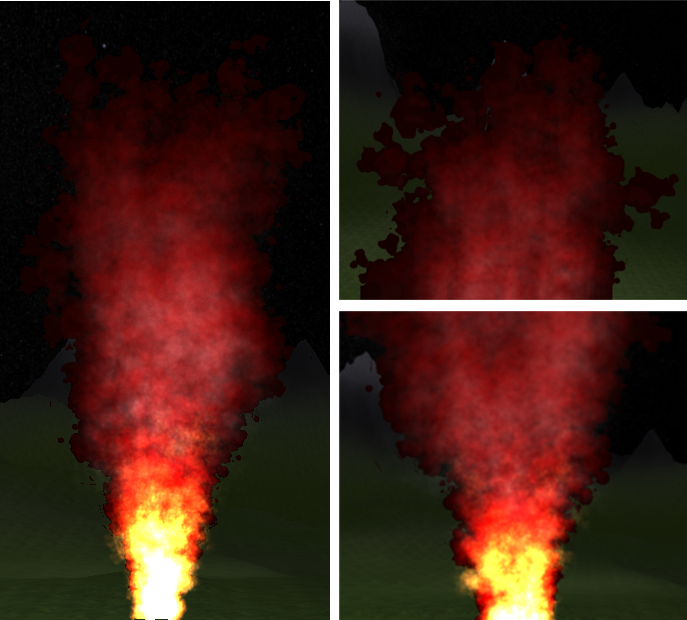
\includegraphics[width=\textwidth]{kepek/redDistortion.png}
 \caption{Gyökvonás nélkül a füstben nagyon gyenge lenne a torzítás.}
 \label{fig:redDistortion}
\end{figure}

Ekkor a \texttt{finalPicture} objektum színpufferében ott van a torzított háttér, így már csak a kirajzolt tüzet kell hozzáadni textúraként. Hogy a mélységtesztet is el tudjam végezni, az előtér és háttér mélységpuffereit is csatolni kell hozzá. A \texttt{draw} metódusa a képernyőre renderel ki a \texttt{blendPictures.fs} árnyaló segítségével. Az mintavételezi a háttér színét, illetve a két mélység értéket. Ha az előtér mélysége nagyobb mint a háttéré, akkor a háttér színe lesz a kimenet, mert az előtér takarásban van. Ha viszont nincs, akkor az előtér megfelelő fragmentjének színét is lekérem, majd azt a háttér színéhez adva (csak az \texttt{RGB} komponenseket) kapom a végső színt. Az alfa értéket a háttér adja.

Így előállt a végső kép, melyen a tűz torzítatlan, a háttér pedig a tűz hőjének függvényében van torzítva (\ref{fig:postprocessing}. ábra jobb alsó képe). Mivel azonban a folyamat során úgyis szert tettünk a mélység értékekre, lehetőség nyílt még egy effekt megvalósítására.


%Soft particles
\subsubsection{Soft particles effekt}
Ahol a tűz a földből előtör, a részecskék élesen ketté vannak vágva. A \textit{soft particles} effekt lényege, hogy az ilyen éles vágásokat kiküszöböljük. Ez akkor is kapóra jön, mikor a tűz nem a földből tör elő, hanem néhány farönkön ég, illetve mikor egy tárgy egésze vagy része a tűzben helyezkedik el. A megoldás nagyon egyszerű: Ahol a részecske mélységértéke közel van a háttere mélységéhez, ott összemossuk vele.

Ehhez kicsit ki kell bővíteni a \texttt{FireParticleSystem} osztályt. Szükség van egy \texttt{addBackgroundDepth} metódusra, mely segítségével a \texttt{renderedFire} FBO-ba való kirajzolás előtt hozzá tudjuk adni a háttér mélység textúrájának azonosítóját az osztályhoz, illetve az \texttt{updateScreenSize}-ra, mely a képernyő méreteit állítja be a shader-nek. Emellett a \texttt{draw} metódusában gondoskodni kell róla, hogy ezt, és az emitter kamerától vett távolságát is átadjuk a \texttt{fireshader} árnyalónak uniform-ként.

A shadert is ki kell egészíteni. Hozzá kell adni a uniform-okat, melyekbe a mélységet és a távolságot (\texttt{backgroundDepth}, \texttt{distanceToCamera}), valamint a képernyő méreteit (\texttt{screenWidth}, \texttt{screenHeigth}) kapjuk. Ezen felül egy fordítónak szóló \texttt{\#define} utasítás segítségével úgy alakítjuk át az árnyalót, hogy azt az effekt megvalósítása nélkül is lehessen használni:
\begin{cpp}
#ifdef SOFTPARTICLES
float bgDepth = texture2D(backgroundDepth, 
		    gl_FragCoord.xy / vec2(screenWidth, screenHeigth)).r;
if (bgDepth > gl_FragCoord.z){
    float distance = bgDepth - gl_FragCoord.z;
    float threshold = 0.1f / pow(distanceToCamera, 2);
    if(distance < threshold)
    {
        float blend = distance / threshold;
        finalColor.a = blend * finalColor.a;
    }
}
else{
    discard;
}
#endif
\end{cpp}
Először a háttér mélységét kérdezem le. Ahhoz, hogy kiderüljön, hogy a képernyő melyik részén vagyunk, a \texttt{gl\_FragCoord} beépített változót hívom segítségül. Ennek $x$ és $y$ koordinátái megadják, hogy mely pixelen vagyunk. Az $x$ koordinátát a képernyő szélességével, az $y$-t a magasságával kell osztani, hogy a megfelelő textúra koordinátákat megkapjuk. A $z$ koordinátája az adott fragment mélységét tárolja, így ezt kell összevetni a mélységpufferből kiolvasott értékkel. Ha a fragment takarásban van akkor el is vethetjük. Ha viszont látszik, akkor ki kell számolni, hogy milyen közel van a háttérhez (\texttt{distance}). Meg kell határozni azt a határt, amin belül el szeretnénk halványítani a részecskét (\texttt{threshold}), azonban mint már említettem korábban, a mélység puffer nem lineáris. Nagyobb távolságok esetén tehát ennek a határnak kisebbnek kell lennie, hogy ne halványuljon el az egész tűz. Ha pedig határon belül vagyunk, akkor a kimenet alfa csatornáján keresztül tudjuk halványítani a részecskét a mélységek távolsága és a halványítási tartomány hányadosa segítségével.

\Aref{fig:softParticle}. ábra felső sorában piros színnel jelöltem az elhalványítandó részeket, az alsó sorában pedig a végeredményt hasonlíthatjuk össze a kiindulási állapottal.

\begin{figure}[h]
 \centering
 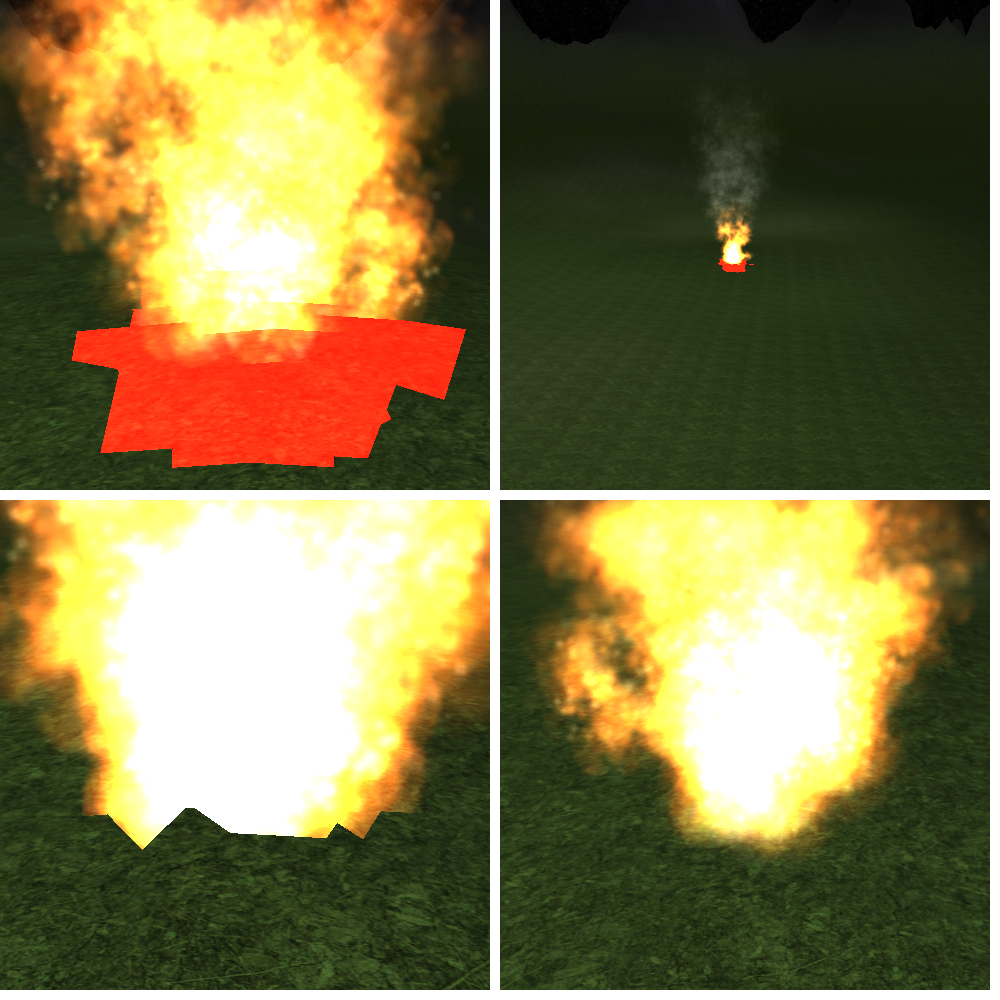
\includegraphics[width=\textwidth]{kepek/softParticle.png}
 \caption{A felső sorban láthatjuk, hogy nagyobb távolságból is megfelelő az elhalványított tartomány.}
 \label{fig:softParticle}
\end{figure}

%% TEST: scale++, speed++, x and z not slowed => explosion? ->nope
%teljesítmény

\subsection{Teljesítmény}
A domborzat és az ég önmagában kirenderelve tehát $400-420$ fps körül teljesít.

% mezei renderelés
\subsubsection{Egyszerű kirajzolás}
Az első részben közvetlenül a képernyőre rajzoltam, post-processing nélkül. A tapasztalatok alapján sokat számít az, hogy mennyi részecskéből áll, és a képernyő mekkora részét teszi ki a jelenet. Utóbbit úgy befolyásoltam a teszt során, hogy különböző távolságokból tekintettem a tűz egészére. Az eredményeket \aref{table:1}. táblázatban gyűjtöttem össze.

\begin{table}[h!]
\centering
\begin{tabular}{ m{10em}|c|c|c|c|c|c|c|c| } 
 $\frac{particle}{seconds}$ & $\frac{450}{3}$ & $\frac{450}{6}$ & $\frac{900}{3}$ & $\frac{900}{6}$ & $\frac{225}{3}$ & $\frac{1500}{3}$ & $\frac{5000}{3}$ & $\frac{10000}{3}$ \\  \hline
 
 normál távolság ($8.3$) & 195 & 172 & 111 & 110 & 255 & 63 & 21 & 10.7\\  \hline
 közvetlen közel ($1.2$) & 110 & 165 & 51 & 108 & 165 & 30 & 7.7 & 4.1\\  \hline
 emitterből felfelé tekintve ($<0.4$) & 30 &  51 & 15.7 & 22.5 & 84 & 11 & 3.3 & 1.9\\ \hline
 messziről ($65.1$) & 410 &  370 & 380 & 355 & 410 & 362 & 240 & 120\\ 
 \hline
\end{tabular}
\caption{Teszt eredmények fps-ben mérve.}
\label{table:1}
\end{table}

A táblázat első sorában a $\frac{\text{maximum részecskeszám}}{\text{részecske élettartam}}$ hányados szerepel, mint változtatott paraméter, mely hányados ezzel egy időben a másodpercenként kibocsátott részecskék száma is. Az ezt követő sorokban fps értékeket találunk adott távolságokból. A kamerát igyekeztem mindig úgy irányítani, hogy a tűz középen legyen, és a lehető legtöbb látszódjon belőle.

Az első oszlopot ($\frac{450}{3}$ részecske/másodperc) választottam kinézet alapján az etalonnak. A normál távolság az a távolság, melyből ennek a tűznek a teteje és az alja nagyjából a képernyő tetejével és aljával esik egybe. A közvetlen közeli esetben vízszintesen nézünk át a jelenségen kamera magasságban ($1.0$), az emitterből felfelé tekintve pedig az egész jelenséget látjuk alulról. A messzi részt pedig egy meghatározott domb tetejéről mértem, ahonnan a tűz magassága nagyjából a képernyő magasságának tizedét tette ki.\\
Ezekből az adatokból azt a következtetést vonom le, hogy nem is az számít igazán, hogy mennyi részecske látszik egyszerre, hanem inkább az, hogy a képernyőnek mekkora részét borítják be.

A második oszlopban a részecskék élettartamát megnöveltem a kétszeresére. Ennek következtében a normál távolságból kisebb a frame rate, de ahogy közeledünk az emitter felé, ez egyre csak nő kb. 3 egységnyi távolságig, majd onnantól kezd csökkenni. Ez azért lehetséges véleményem szerint, mert a képernyőn jobban eloszlanak a részecskék, így közelről kevesebb jelenik meg (így egy fragmentet átlagban kevesebbszer is kell feldolgozni), de nem foglalnak el nagyobb területet mint az etalon esetnél. Az emitterből felfelé tekintve is jobb teljesítményt kapunk, valószínűleg azért, mert a részecskék nagyobb magasságban vannak eloszlatva, és a távolabbiakat kisebb erőforrás igénnyel rajzolja ki. Nagy távolságból többet romlott a teljesítmény, ami azért lehetséges, mert tovább élnek a részecskék, nagyobb utat tesznek meg, így ugyanakkora távolságból nagyobb területet fednek le a képernyőn.

A harmadik oszlopban a részecskék maximális száma kétszer akkora, mint az etalon esetben. Ez már inkább meglátszik a teljesítményben, ugyanis az majdnem a felére esett vissza, kivéve nagyobb távolságból.

A negyedik esetben az időt is megdupláztam, és hasonló jellegzetességeket mutat az első kettő és az utolsó két teszt. Csupán az élettartam növelésének hatására ritkul a tűz, így közvetlen közelből jobb a teljesítmény, de messzebbről kicsivel rosszabb. 

Az ötödik tesztben az etalon részecskék számát megfeleztem, ez jelentős teljesítménynövekedést okozott, főleg az emitterből felfelé tekintve.

A hatodik esetben a maximális részecskeszám 1500 volt. Tisztes távolból még teljesen elfogadható teljesítményt nyújt, tekintve hogy egy monitor általában 60 Hz-es frekvencián frissíti a képet, 60 fps-nél többet nem is érdemes produkálni. Azonban ha azt tekintjük, hogy a domborzatot és az eget leszámítva a tűz mellett üres a tér, akkor egy díszítő funkciót ellátó objektum megjelenítésére ez egy kicsit drága választás.

Az utolsó két oszlop már csak az érdekesség kedvéért készült. Az $5000$ részecskés esetben már normál távolságból is darabos a jelenet, az elfogadható sebesség nagyjából 30 fps körül van, amelyet minimum 10 egységnyi távolság esetén ér el. A részecskeszám kétszeresére növelése itt is durván a teljesítmény feleződését mutatta.

% postprocessing
\subsubsection{Kirajzolás és post-processing}
A következő teszteket post-processing kíséretében végeztem el, azonos szempontok alapján. Az eredményeket \aref{table:2}. táblázatban lehet megtekinteni.

\begin{table}[h!]
\centering
\begin{tabular}{ m{10em}|C{1cm}|C{1cm}|C{1cm}|C{1cm}|C{1cm}|C{1cm}|C{1cm}|C{1cm}| } 
 $\frac{particle}{seconds}$ & $\frac{450}{3}$ & $\frac{450}{6}$ & $\frac{900}{3}$ & $\frac{225}{3}$ & $\frac{1500}{3}$ & $\frac{5000}{3}$ & $\frac{10000}{3}$ \\  \hline
 
 normál távolság ($8.3$)                   & 124  (195) & 124 (172)  & 86 (111)     & 168 (255)  & 57 (63)     & 20 (21) & 10.5 (10.7) \\  \hline
 közvetlen közel ($1.2$)                    & 89 (110)   & 120 (165)  & 45 (51)       & 115 (165)  & 29 (30)     & 8.8 (7.7) & 4.2 (4.1) \\  \hline
 emitterből felfelé tekintve ($<0.4$) & 27 (30)     &  48 (51)    & 14.5 (15.7) & 58 (84)      & 10.2 (11)  & 3.2 (3.3) & 1.2 (1.9)  \\ \hline
 messziről ($65.1$)                            & 230 (410) &  220 (370) & 225 (380)   & 232 (410)  & 205 (362)   & 180 (240) & 100 (120) \\ 
 \hline
\end{tabular}
\caption{Zárójelben az előző teszt eredményei szerepelnek.}
\label{table:2}
\end{table}

Ha összevetjük az előző teszt eredményeivel a mostaniakat, akkor nem meglepő módon arra jutunk, hogy a teljesítmény egyértelműen romlott, ami viszont érdekesebb, hogy nem egyenlő arányban. Első ránézésre szembetűnő, hogy a részecskeszám növelése mellett a post-processing egyre kisebb arányban rontja a teljesítményt. Ez logikus, hiszen a post-processing műveletekre a részecskék száma nincs különösebb hatással, így azt tulajdonképpen konstans költségnek is tekinthetjük. Ez pedig eltörpül akkora költségek mellett, mint például $10000$ részecske kirajzolása.

Ahogy pedig a tűz kirajzolásának költségei csökkennek (például messzebbről szemléljük a jelenséget), úgy egyre nagyobb arányban jelentkezik a post-processing számításigénye. Ezt láthatjuk az utolsó sorban, ahol a legnagyobb a teljesítmény abszolút értékű esése.

Minél nagyobb felületet borít be a képernyőn a tűz, annál több fragment esetén kell elvégezni az eltolást, így elvileg nő a post-processing számításigénye. Ezt leginkább a középső két sorban lehetne tapasztalni, de a részecskék megjelenítésének annyival nő a költsége, hogy a post-processing többletköltsége nem mutatkozik jelentősen.

Ha egy virtuális környezet hangulatát szeretnénk tűzzel javítani, akkor el kell dönteni, hogy mennyire fontos a valóságosság, és mekkora kapacitást szánunk a díszítő elemekre megjelenítésére. Véleményem szerint a látvány post-processing nélkül is elfogadható, 3 másodperces élettartam mellett pedig 225 részecskével is egészen reális tüzet lehet megjeleníteni anélkül, hogy súlyosabb erőforrásigényt rónánk a hardverre. Ha fontos a szép látvány, akkor 450 részecskével és post-processing effektekkel még továbbra is elfogadható marad a számításigény, főleg ha a környezetet és esetleg a tüzet is további lépésekkel egyszerűsítjük. Ilyen lépés lehet a tesszelláció, melynek során a távolabbi objektumok vertex számát és komplexitását csökkentjük. Kellő távolságból a részecskerendszert akár egy egyszerű, kétdimenziós billboard alapú tűzzel is helyettesíthetjük.









\Chapter{Eredmények bemutatása}

% TODO: Részletesen bemutatni, hogy a renderelés, animáció milyen eredményt ad!


\Chapter{Összegzés}

%feladat
A dolgozat fő célja a tűz és a hozzá kapcsolódó jelenségek megvalósításának áttekintése volt a számítógépi grafikában. Az elérhető játékmotorok vizsgálatán keresztül próbáltam betekintést nyerni a tűz megjelenítéssel kapcsolatos problémáinak megoldásaira, illetve ezeket vizsgáltam valószerűség és számításigény tekintetében. Elsősorban a valós idejű megjelenítéssel foglalkoztam, de kitértem néhány valós időben nem feldogozható módszerre is. Egyes módszereket magam is implementáltam.

%eredmények
% néhány motor áttekintve, történeti ismeretek, praktikák megismerése
%tűz fizikájának, folyamatainak megismerése
% különböző módszerek és lehetőségek feltárása, ötletelés szintjén
% billboard tűz, particle system, post processing implementáció
A legkorábbi játékmotorok vizsgálatával kezdtem, majd időrendben haladtam a modernebb, számításigényesebb megvalósítások irányába. A kutatás során a motorokkal kapcsolatban történeti ismeretekre is szert tettem, illetve több, grafikában alkalmazott praktikát megismertem a számításigény csökkentése érdekében, habár ezek minden részletét már nem fejtettem ki a dolgozatban. 

Megismertem a tűz fizikai és kémiai hátterét, mely segített, hogy a jelenséget kód formájában is meg tudjam fogalmazni. Különféle módszereket mutattam be a megvalósításra vonatkozóan, ezeken elmélkedve és saját ötletekkel kiegészítve több lehetőséget is feltártam az adott módszerekkel kapcsolatban a valószerűség javítása érdekében.
Ezek közül néhányat magam is sikeresen implementáltam, melyet részletesen dokumentáltam a rész- és végeredmények bemutatásával egyetemben. 

%tapasztalatok
% játékmotorokon elmenni nem piskóta, árnyalók végtelen lehetőségei, nehézkes debuggolása, átlátszóság és kirajzolás sorrendje kemény dió, jobb teljesítményhez hardverközelebbi megoldások, ismeretek szükségesek, kreativitás > erőforrások
A dolgozat írása közben azt tapasztaltam, hogy a legapróbb részletekben rejlő hiba is komoly akadályokat jelenthet. Ezen hibák feltárása rengeteg utánajárást és kutatást igényelt, legtöbbször a dokumentációknak, és néha a vak szerencsének köszönhettem a megoldást. A korábbi játékmotorok elemzése során rájöttem, hogy a kreativitás képes felülmúlni a hardver képességeit, azonban ehhez komoly jártasság szükséges az informatikai technológiák területén. 


%fejlesztési lehetőségek
%optimalizálás, tűz elmosás, volumetrikus/voxel tűz, fizikai modellek, tűz terjedés-gyulladás-kioltás, interakció más tárgyakkal, fény és hang jelenségek, parázs darabkák
Számos lehetőség van még az implementációim javítására. A post-processing segítségével például a tűz kinézetén is lehetne javítani, a részecskék életciklusa pedig elbírna egy fizikailag élethűbb modellt. A fény és hangjelenségek csatolása, illetve a más objektumokkal történő interakció megvalósítása szintén segíthetné a hitelesebb megjelenítést. 

%\begin{figure}[h]
% \centering
% 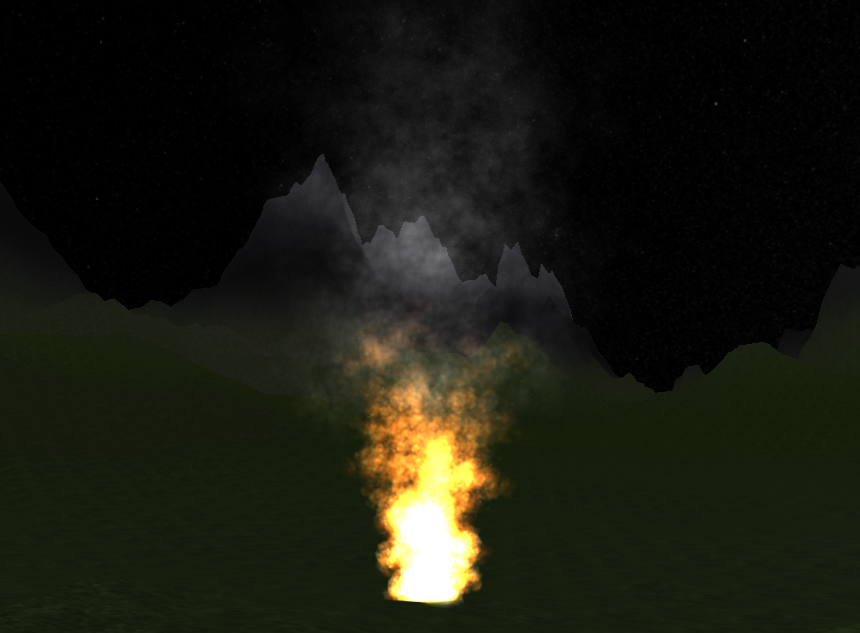
\includegraphics[width=\textwidth]{kepek/particleFinal.png}
% \caption{A végső eredmény hőből fakadó torzítással, és soft particle megvalósítással.}
% \label{fig:particleFinal}
%\end{figure}


\Chapter{Summary}

The main purpose of the thesis was to explore the implementation possibilities of the fire and the related phenomena in computer graphics. I tried to get an insight into the solutions of the problems related to fire rendering through investigation of available game engines, and examined these methods with respect to realism and computational costs. I dealt with real time rendering in the first place, but also investigated some methods that cannot be computed in real time. I have implemented some of the former ones as well.

I started the investigation with some of the earliest game engines, then moved on to more modern and computationally intense realizations in chronological order. Meanwhile, I also gathered some knowledge in the history of the game engines, and learned about some practices to reduce computational costs of the applications. 

I learned about the physical and chemical background of the fire, which helped me to be able to program the phenomenon. I wrote about various methods for rendering fire and made up some ideas to improve realism. Some of these were also successfully implemented by me, which I documented along with some partial and final results.

While working on the thesis I found, that even the smallest details can cause huge problems. Their solutions required a lot of research, most of the time I was helped out by documentations, and sometimes I solved problems through dumb luck. While analyzing the older game engines I discovered, that you can fight the limitations of the hardware with creativity, although that requires advanced skills.

There are still lots of possibilities for improvement. The appearance of the fire could be enhanced using post-processing, and the particles could use some more realistic physics. Attaching light and sound, along with the possibility to interact with fire would be highly beneficial for realism.



\Chapter{CD-melléklet tartalma}

A szakdolgozatom mellé egy darab CD tartozik, amely a következő adatokat tartalmazza:
\begin{itemize}
\item \texttt{dolgozat.pdf}: a dolgozat PDF formátumban.
\item \texttt{Dolgozat} katalógus: a szakdolgozat fájljai.
\item \texttt{SpriteFire} katalógus: a billboard alapú tűz forrásfájljai és egy futtatható állománya.
\item \texttt{ParticleFire} katalógus: a részecskerendszer alapú tűz forrásfájljai és egy futtatható állománya.
\item \texttt{Eredmenyek} katalógus: képernyő videók az eredmények bemutatása céljából.
\item \texttt{osszegzes.pdf}, \texttt{osszegzes.text}: a dolgozat magyar nyelvű összefoglalója.
\item \texttt{summary.pdf}, \texttt{summary.tex}: a dolgozat angol nyelvű összefoglalója.
\end{itemize}

A futtatható fájlok Windows operációs rendszer alatt használhatók.\\
A forráskódokban a tűz implementációk a \texttt{fire.hpp} és \texttt{fire.cpp} fájlokban találhatóak, a kirajzolás a \texttt{main.cpp} fájl \texttt{display} függvényében található. A részecske tűz forrásai közül még a \texttt{postprocessor.hpp} és \texttt{postprocessor.cpp} fájlok lehetnek érdekesek. 

A SpriteFire demóban a + és - gombokkal a tűz sebességét lehet állítani.\\
A ParticleFire demóban az `m' betűvel lehet a szelet be- és kikapcsolni.

%1.	Egy kötelezően Dolgozat nevű katalógus, amely az alábbiakat tartalmazza: 
%      a.	A dolgozatot tartalmazó fájl, a használt szerkesztő formátumában (pl. .docx)
%      b.	A dolgozatot tartalmazó fájl, PDF formátumban, .pdf kiterjesztéssel 
%      c.	A kiírás, külön fájlban. 
%      d.	A dolgozatból kiemelve, egy-egy külön fájlban a magyar és az angol nyelvű összefoglalót, a használt szerkesztő (pl. .docx) formátumában és PDF formátumban is. 

%2.	További katalógusokban minden olyan anyag, ami a dolgozathoz tartozik (forráskódok, működő demó, nagyobb méretű mellékletek stb.). Ez a tartalom természetesen a munka jellegétől függően nagyon sokféle lehet, célszerű megbeszélni a tervezésvezetővel.




\begin{thebibliography}{x}
\addcontentsline{toc}{chapter}{\bibname}

\bibitem{wikiGameEngine}
  Wikipedia,
  \textit{Game engine}, \\
  \url{https://en.wikipedia.org/wiki/Game_engine}

\bibitem{steinemannFire}
  Denis Steinemann,
  \textit{Simulation and Animation of Fire}, \\
  A presentation in Seminar on Physically-based Methods for 3D-Games and Medical Applications
  
\bibitem{firestarter}
  Marc de Kruijf,
  \textit{firestarter – A Real-Time Fire Simulator}

\bibitem{ArNiStructuralModeling}
 Arnauld Lamorlette, Nick Foster,
 \textit{Structural Modeling of Flames for a Production Environment}

\bibitem{wikiQuake}
 Wikipedia, 
 \textit{Quake engine},\\
 \url{https://en.wikipedia.org/wiki/Quake_engine}
 
\bibitem{MDLformat}
 David Henry, 
 \textit{MDL file format (Quake's models)},\\
 \url{http://tfc.duke.free.fr/coding/mdl-specs-en.html}

\bibitem{wikiQuake2}
 Wikipedia, 
 \textit{Quake II engine},\\
 \url{https://en.wikipedia.org/wiki/Quake_II_engine}

\bibitem{fsQuake2}
 Fabien Sanglard, 
 \textit{Quake 2 Source Code Review},\\
 \url{http://fabiensanglard.net/quake2/quake2_opengl_renderer.php}

\bibitem{MD2format}
 David Henry, 
 \textit{MD2 file format (Quake 2's models)},\\
 \url{http://tfc.duke.free.fr/coding/md2-specs-en.html}

\bibitem{quake3shaderManual}
  Paul Jaquays, Brian Hook
  \textit{Quake III Arena Shader Manual},
  December 23, 1999

\bibitem{fsQuake3}
  Fabien Sanglard, 
  \textit{Quake 3 Source Code Review},\\
  \url{http://fabiensanglard.net/quake3/renderer.php}

\bibitem{wikiQuake3}
 Wikipedia, 
 \textit{id Tech 3},\\
 \url{https://en.wikipedia.org/wiki/Id_Tech_3}

\bibitem{wikUE4}
 Wikipedia, 
 \textit{Unreal Engine},\\
 \url{https://en.wikipedia.org/wiki/Unreal_Engine#Unreal_Engine_4}

\bibitem{UEngineFireExample}
 Unreal Engine Documentation, 
 \textit{Fire Examples},\\
 \url{https://docs.unrealengine.com/en-us/Resources/Showcases/Effects/FireExamples}

\bibitem{firePhysics1}
 Anne Marie Helmenstine, Ph.D., 
 \textit{Is Fire a Gas, Liquid, or Solid?},\\
 \url{https://www.thoughtco.com/what-state-of-matter-is-fire-604300}

\bibitem{firePhysics2}
 Anne Marie Helmenstine, Ph.D., 
 \textit{What Is Fire Made Of?},\\
 \url{https://www.thoughtco.com/what-is-fire-made-of-607313}

\bibitem{swhThreeDimensionalReconst}
  Samuel William Hasino,
  \textit{Three-Dimensional Reconstruction of Fire from Images},
 2002.

\bibitem{wikiOGL}
 Wikipedia, 
 \textit{OpenGL},\\
 \url{https://en.wikipedia.org/wiki/OpenGL}
 
 \bibitem{freeGlut}
 Freeglut, 
 \textit{Official page},\\
 \url{http://freeglut.sourceforge.net}
 
  \bibitem{glew}
 The OpenGL Extension Wrangler Library, 
 \textit{Official page},\\
 \url{http://glew.sourceforge.net}
 
  \bibitem{glm}
 OpenGL Mathematics, 
 \textit{Official page},\\
 \url{https://glm.g-truc.net/0.9.8/index.html}

  \bibitem{soil}
Simple OpenGL Image Library, 
 \textit{Official page},\\
 \url{https://www.lonesock.net/soil.html}

\end{thebibliography}



\pagestyle{empty}
\vspace*{1cm}  
\begin{center}
\large\textsc{\bfseries Eredetiségi Nyilatkozat}
\end{center}
\vspace*{2cm}  

Alulírott \textbf{Fodor Tamás János}; Neptun-kód: \texttt{OGL04D} a Miskolci Egyetem Gépészmérnöki és Informatikai Karának végzõs mérnökinformatikus szakos hallgatója ezennel büntetõjogi és fegyelmi felelõsségem tudatában nyilatkozom és aláírásommal igazolom, hogy
\textit{Tűzzel kapcsolatos jelenségek grafikus megjelenítése}
címû szakdolgozatom/diplomatervem saját, önálló munkám; az abban hivatkozott szakirodalom
felhasználása a forráskezelés szabályai szerint történt.\\

Tudomásul veszem, hogy szakdolgozat esetén plágiumnak számít:
\begin{itemize}
\item szószerinti idézet közlése idézõjel és hivatkozás megjelölése nélkül;
\item tartalmi idézet hivatkozás megjelölése nélkül;
\item más publikált gondolatainak saját gondolatként való feltüntetése.
\end{itemize}

Alulírott kijelentem, hogy a plágium fogalmát megismertem, és tudomásul veszem, hogy
plágium esetén szakdolgozatom visszautasításra kerül.

\vspace*{3cm}

\noindent Miskolc, \hbox to 2cm{\dotfill} év \hbox to 2cm{\dotfill} hó \hbox to 2cm{\dotfill} nap

\vspace*{3cm}

\hspace*{8cm}\begin{tabular}{c}
\hbox to 6cm{\dotfill}\\
Hallgató
\end{tabular}


\end{document}
